% Options for packages loaded elsewhere
\PassOptionsToPackage{unicode}{hyperref}
\PassOptionsToPackage{hyphens}{url}
%
\documentclass[
]{book}
\usepackage{lmodern}
\usepackage{amssymb,amsmath}
\usepackage{ifxetex,ifluatex}
\ifnum 0\ifxetex 1\fi\ifluatex 1\fi=0 % if pdftex
  \usepackage[T1]{fontenc}
  \usepackage[utf8]{inputenc}
  \usepackage{textcomp} % provide euro and other symbols
\else % if luatex or xetex
  \usepackage{unicode-math}
  \defaultfontfeatures{Scale=MatchLowercase}
  \defaultfontfeatures[\rmfamily]{Ligatures=TeX,Scale=1}
\fi
% Use upquote if available, for straight quotes in verbatim environments
\IfFileExists{upquote.sty}{\usepackage{upquote}}{}
\IfFileExists{microtype.sty}{% use microtype if available
  \usepackage[]{microtype}
  \UseMicrotypeSet[protrusion]{basicmath} % disable protrusion for tt fonts
}{}
\makeatletter
\@ifundefined{KOMAClassName}{% if non-KOMA class
  \IfFileExists{parskip.sty}{%
    \usepackage{parskip}
  }{% else
    \setlength{\parindent}{0pt}
    \setlength{\parskip}{6pt plus 2pt minus 1pt}}
}{% if KOMA class
  \KOMAoptions{parskip=half}}
\makeatother
\usepackage{xcolor}
\IfFileExists{xurl.sty}{\usepackage{xurl}}{} % add URL line breaks if available
\IfFileExists{bookmark.sty}{\usepackage{bookmark}}{\usepackage{hyperref}}
\hypersetup{
  pdftitle={Introdução ao R com aplicações em biodiversidade e conservação},
  hidelinks,
  pdfcreator={LaTeX via pandoc}}
\urlstyle{same} % disable monospaced font for URLs
\usepackage{color}
\usepackage{fancyvrb}
\newcommand{\VerbBar}{|}
\newcommand{\VERB}{\Verb[commandchars=\\\{\}]}
\DefineVerbatimEnvironment{Highlighting}{Verbatim}{commandchars=\\\{\}}
% Add ',fontsize=\small' for more characters per line
\usepackage{framed}
\definecolor{shadecolor}{RGB}{248,248,248}
\newenvironment{Shaded}{\begin{snugshade}}{\end{snugshade}}
\newcommand{\AlertTok}[1]{\textcolor[rgb]{0.94,0.16,0.16}{#1}}
\newcommand{\AnnotationTok}[1]{\textcolor[rgb]{0.56,0.35,0.01}{\textbf{\textit{#1}}}}
\newcommand{\AttributeTok}[1]{\textcolor[rgb]{0.77,0.63,0.00}{#1}}
\newcommand{\BaseNTok}[1]{\textcolor[rgb]{0.00,0.00,0.81}{#1}}
\newcommand{\BuiltInTok}[1]{#1}
\newcommand{\CharTok}[1]{\textcolor[rgb]{0.31,0.60,0.02}{#1}}
\newcommand{\CommentTok}[1]{\textcolor[rgb]{0.56,0.35,0.01}{\textit{#1}}}
\newcommand{\CommentVarTok}[1]{\textcolor[rgb]{0.56,0.35,0.01}{\textbf{\textit{#1}}}}
\newcommand{\ConstantTok}[1]{\textcolor[rgb]{0.00,0.00,0.00}{#1}}
\newcommand{\ControlFlowTok}[1]{\textcolor[rgb]{0.13,0.29,0.53}{\textbf{#1}}}
\newcommand{\DataTypeTok}[1]{\textcolor[rgb]{0.13,0.29,0.53}{#1}}
\newcommand{\DecValTok}[1]{\textcolor[rgb]{0.00,0.00,0.81}{#1}}
\newcommand{\DocumentationTok}[1]{\textcolor[rgb]{0.56,0.35,0.01}{\textbf{\textit{#1}}}}
\newcommand{\ErrorTok}[1]{\textcolor[rgb]{0.64,0.00,0.00}{\textbf{#1}}}
\newcommand{\ExtensionTok}[1]{#1}
\newcommand{\FloatTok}[1]{\textcolor[rgb]{0.00,0.00,0.81}{#1}}
\newcommand{\FunctionTok}[1]{\textcolor[rgb]{0.00,0.00,0.00}{#1}}
\newcommand{\ImportTok}[1]{#1}
\newcommand{\InformationTok}[1]{\textcolor[rgb]{0.56,0.35,0.01}{\textbf{\textit{#1}}}}
\newcommand{\KeywordTok}[1]{\textcolor[rgb]{0.13,0.29,0.53}{\textbf{#1}}}
\newcommand{\NormalTok}[1]{#1}
\newcommand{\OperatorTok}[1]{\textcolor[rgb]{0.81,0.36,0.00}{\textbf{#1}}}
\newcommand{\OtherTok}[1]{\textcolor[rgb]{0.56,0.35,0.01}{#1}}
\newcommand{\PreprocessorTok}[1]{\textcolor[rgb]{0.56,0.35,0.01}{\textit{#1}}}
\newcommand{\RegionMarkerTok}[1]{#1}
\newcommand{\SpecialCharTok}[1]{\textcolor[rgb]{0.00,0.00,0.00}{#1}}
\newcommand{\SpecialStringTok}[1]{\textcolor[rgb]{0.31,0.60,0.02}{#1}}
\newcommand{\StringTok}[1]{\textcolor[rgb]{0.31,0.60,0.02}{#1}}
\newcommand{\VariableTok}[1]{\textcolor[rgb]{0.00,0.00,0.00}{#1}}
\newcommand{\VerbatimStringTok}[1]{\textcolor[rgb]{0.31,0.60,0.02}{#1}}
\newcommand{\WarningTok}[1]{\textcolor[rgb]{0.56,0.35,0.01}{\textbf{\textit{#1}}}}
\usepackage{longtable,booktabs}
% Correct order of tables after \paragraph or \subparagraph
\usepackage{etoolbox}
\makeatletter
\patchcmd\longtable{\par}{\if@noskipsec\mbox{}\fi\par}{}{}
\makeatother
% Allow footnotes in longtable head/foot
\IfFileExists{footnotehyper.sty}{\usepackage{footnotehyper}}{\usepackage{footnote}}
\makesavenoteenv{longtable}
\usepackage{graphicx,grffile}
\makeatletter
\def\maxwidth{\ifdim\Gin@nat@width>\linewidth\linewidth\else\Gin@nat@width\fi}
\def\maxheight{\ifdim\Gin@nat@height>\textheight\textheight\else\Gin@nat@height\fi}
\makeatother
% Scale images if necessary, so that they will not overflow the page
% margins by default, and it is still possible to overwrite the defaults
% using explicit options in \includegraphics[width, height, ...]{}
\setkeys{Gin}{width=\maxwidth,height=\maxheight,keepaspectratio}
% Set default figure placement to htbp
\makeatletter
\def\fps@figure{htbp}
\makeatother
\setlength{\emergencystretch}{3em} % prevent overfull lines
\providecommand{\tightlist}{%
  \setlength{\itemsep}{0pt}\setlength{\parskip}{0pt}}
\setcounter{secnumdepth}{5}
\usepackage{booktabs}
\usepackage[]{natbib}
\bibliographystyle{apalike}

\title{Introdução ao R com aplicações em biodiversidade e conservação}
\author{}
\date{\vspace{-2.5em}2020-09-17}

\begin{document}
\maketitle

{
\setcounter{tocdepth}{1}
\tableofcontents
}
\hypertarget{pruxe9-requisitos}{%
\chapter{Pré-requisitos}\label{pruxe9-requisitos}}

\hypertarget{estatuxedstica-buxe1sica}{%
\chapter{Estatística básica}\label{estatuxedstica-buxe1sica}}

\hypertarget{teste-t-de-student-para-duas-amostras-independentes}{%
\section{Teste T (de Student) para duas amostras independentes}\label{teste-t-de-student-para-duas-amostras-independentes}}

\hypertarget{backgorund-da-anuxe1lise}{%
\subsection{Backgorund da análise}\label{backgorund-da-anuxe1lise}}

Uma das perguntas mais comum em estatística é saber se há diferença entre as médias de dois grupos ou tratamentos. Para responder esta pergunta, William Sealy Gosset, químico da cervejaria Guinness, em 1908 desenvolveu o Teste T que é uma estátistica que segue uma distribuição t de Student para rejeitar ou não uma hipótese nula de médias iguais entre os grupos.

\begin{quote}
\[ t = \frac{(\bar{X}_1 - \bar{X}_2)}{\sqrt{\frac{2S^2_p}{n}}}\]
\end{quote}

Onde:

\begin{itemize}
\item
  \(\bar{X}\)1 - \(\bar{X}\)2 = diferença entre as médias das duas amostras,
\item
  S2p = desvio padrão das amostras,
\item
  \emph{n} = tamanho das amostras.
\end{itemize}

\begin{quote}
\hypertarget{premissas-do-teste-t}{%
\subsubsection{Premissas do Teste t :}\label{premissas-do-teste-t}}

\begin{itemize}
\tightlist
\item
  As amostras devem ser independentes;
\item
  As unidades amostrais são selecionadas aleatoriamente;
\item
  Distribuição normal (gaussiana) dos resíduos. \textbf{Observação:} Zar (2010, p.~136) indica que o Test T é robusto mesmo com moderada violação da normalidade, principalmente se o tamanho amostral for alto.
\item
  Homogeneidade da variância. \textbf{Observação.} Caso as variâncias não sejam homogêneas, isso deve ser informado na linha de comando, pois o denominador da fórmula acima será corrigido.
\end{itemize}
\end{quote}

~

\hypertarget{exemplo-pruxe1tico-1---teste-t-para-duas-amostras-com-variuxe2ncias-iguais}{%
\subsubsection{Exemplo prático 1 - Teste T para duas amostras com variâncias iguais}\label{exemplo-pruxe1tico-1---teste-t-para-duas-amostras-com-variuxe2ncias-iguais}}

\hypertarget{explicauxe7uxe3o-dos-dados}{%
\paragraph{Explicação dos dados}\label{explicauxe7uxe3o-dos-dados}}

Neste exemplo avaliaremos o comprimento rostro-cloacal (CRC em milímetros) de machos de \emph{Physalaemus natteri} (Anura:Leptodactylidae) amostrados em diferentes estações do ano com armadilhas de interceptação e queda na região noroeste do estado de São Paulo (da Silva \& Rossa-Feres 2010).

\textbf{Pergunta:}

\begin{quote}
O CRC dos machos de \emph{P. nattereri} é maior na estação chuvosa do que na estação seca?
\end{quote}

\textbf{Predições}

\begin{quote}
O CRC dos machos será maior na estação chuvosa porque há uma vantangem seletiva para os indivíduos maiores durante a atividade reprodutiva.
\end{quote}

\textbf{Variáveis}

\begin{itemize}
\tightlist
\item
  Variáveis preditoras

  \begin{itemize}
  \tightlist
  \item
    Dataframe com os indivíduos (unidade amostral) nas linhas e CRC (mm - variável resposta contínua) e estação (variável preditora categórica) como colunas.
  \end{itemize}
\end{itemize}

\textbf{Checklist}

\begin{itemize}
\tightlist
\item
  Verificar se o seu dataframe está com as unidades amostrais nas linhas e variáveis preditores nas colunas
\end{itemize}

\hypertarget{anuxe1lise}{%
\subsection{Análise}\label{anuxe1lise}}

Calculo do Teste T para duas amostras independentes com variâncias iguais

\begin{Shaded}
\begin{Highlighting}[]
\CommentTok{## IMPORTANDO OS DADOS}
\CommentTok{#************************}
\NormalTok{CRC_PN_macho <-}\StringTok{ }\NormalTok{ecodados}\OperatorTok{::}\NormalTok{teste_t_var_igual}
\CommentTok{# verificar se o dataframe foi lido corretamente e se não há erros}
\CommentTok{# Esses comandos são úteis para planilhas grandes}
\KeywordTok{head}\NormalTok{(CRC_PN_macho) }\CommentTok{# mostra as seis primeiras linhas da planilha}
\end{Highlighting}
\end{Shaded}

\begin{verbatim}
##    CRC Estacao
## 1 3.82 Chuvosa
## 2 3.57 Chuvosa
## 3 3.67 Chuvosa
## 4 3.72 Chuvosa
## 5 3.75 Chuvosa
## 6 3.83 Chuvosa
\end{verbatim}

\begin{Shaded}
\begin{Highlighting}[]
\KeywordTok{tail}\NormalTok{(CRC_PN_macho) }\CommentTok{# mostra as seis últimas linhas da planilha}
\end{Highlighting}
\end{Shaded}

\begin{verbatim}
##     CRC Estacao
## 46 3.16    Seca
## 47 3.48    Seca
## 48 3.48    Seca
## 49 3.49    Seca
## 50 3.51    Seca
## 51 3.30    Seca
\end{verbatim}

\begin{Shaded}
\begin{Highlighting}[]
\CommentTok{# TESTE NORMALIDADE}
\CommentTok{#************************}
\CommentTok{## Verificando normalidade usando QQ-plot}
\CommentTok{## Os pontos não podem fugir da reta criando formas como U}
\NormalTok{residuos <-}\StringTok{ }\KeywordTok{lm}\NormalTok{(CRC }\OperatorTok{~}\StringTok{ }\NormalTok{Estacao, }\DataTypeTok{data =}\NormalTok{ CRC_PN_macho)}
\KeywordTok{library}\NormalTok{(}\StringTok{"car"}\NormalTok{)}
\KeywordTok{qqPlot}\NormalTok{(residuos)}
\end{Highlighting}
\end{Shaded}

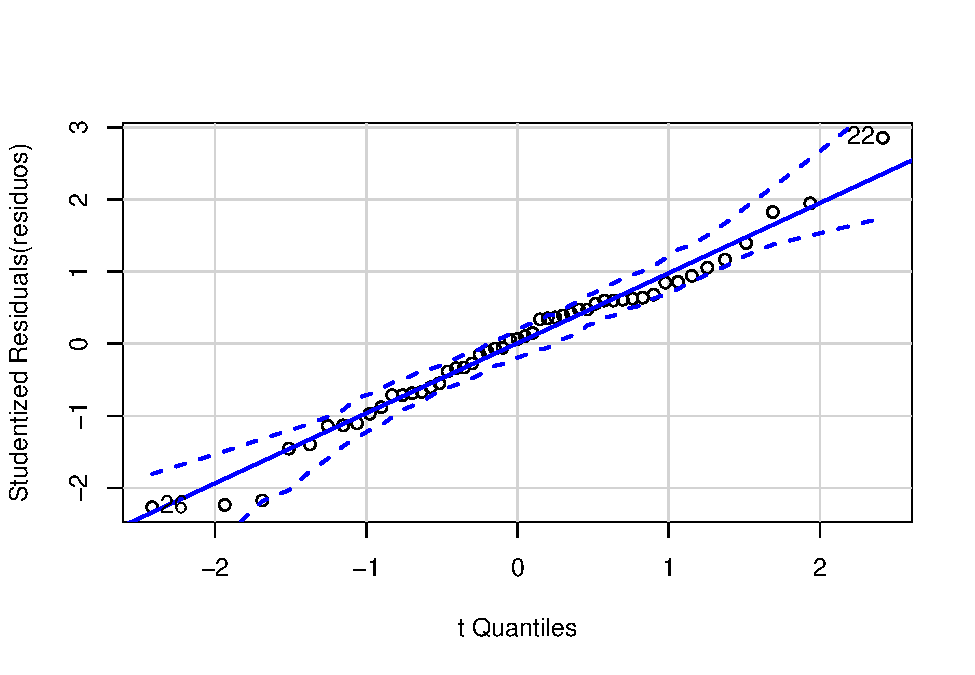
\includegraphics{livro_r_ecologia_files/figure-latex/unnamed-chunk-1-1.pdf}

\begin{verbatim}
## [1] 22 26
\end{verbatim}

\begin{Shaded}
\begin{Highlighting}[]
\CommentTok{## Outra possibilidade é usar o teste de Shapiro-Wilk para verificar normalidade}
\CommentTok{## Hipótese nula que a distribuição é normal }
\CommentTok{## valor de p < 0.05 significa que os dados não apresentam distribuição normal}
\CommentTok{## valor de p > 0.05 significa que os dados apresentam distribuição normal}
\KeywordTok{shapiro.test}\NormalTok{ (CRC_PN_macho}\OperatorTok{$}\NormalTok{CRC) }
\end{Highlighting}
\end{Shaded}

\begin{verbatim}
## 
## 	Shapiro-Wilk normality test
## 
## data:  CRC_PN_macho$CRC
## W = 0.95559, p-value = 0.05417
\end{verbatim}

\begin{Shaded}
\begin{Highlighting}[]
\CommentTok{# TESTE DE HOMOGENEIDADE DA VARIÂNCIA}
\CommentTok{#***************************************}
\CommentTok{## Hipótese nula que a variância é homogênea}
\CommentTok{## valor de p < 0.05 significa que os dados não apresentam homogeneidade}
\CommentTok{## valor de p > 0.05 significa que os dados apresentam homogeneidade}
\KeywordTok{library}\NormalTok{(car)}
\KeywordTok{leveneTest}\NormalTok{(CRC }\OperatorTok{~}\StringTok{ }\NormalTok{Estacao, }\DataTypeTok{data =}\NormalTok{ CRC_PN_macho)}
\end{Highlighting}
\end{Shaded}

\begin{verbatim}
## Levene's Test for Homogeneity of Variance (center = median)
##       Df F value Pr(>F)
## group  1  1.1677 0.2852
##       49
\end{verbatim}

\begin{Shaded}
\begin{Highlighting}[]
\CommentTok{# TESTE T AMOSTRAS INDEPENDENTES E VARIÂNCIAS IGUAIS}
\CommentTok{#******************************************************888}
\KeywordTok{t.test}\NormalTok{(CRC }\OperatorTok{~}\StringTok{ }\NormalTok{Estacao, }\DataTypeTok{data =}\NormalTok{ CRC_PN_macho, }\DataTypeTok{var.equal =} \OtherTok{TRUE}\NormalTok{)}
\end{Highlighting}
\end{Shaded}

\begin{verbatim}
## 
## 	Two Sample t-test
## 
## data:  CRC by Estacao
## t = 4.1524, df = 49, p-value = 0.000131
## alternative hypothesis: true difference in means is not equal to 0
## 95 percent confidence interval:
##  0.2242132 0.6447619
## sample estimates:
## mean in group Chuvosa    mean in group Seca 
##              3.695357              3.260870
\end{verbatim}

Visualizar os resultados em gráfico

\begin{Shaded}
\begin{Highlighting}[]
\KeywordTok{library}\NormalTok{(ggplot2)}
\KeywordTok{ggplot}\NormalTok{(}\DataTypeTok{data =}\NormalTok{ CRC_PN_macho, }\KeywordTok{aes}\NormalTok{(}\DataTypeTok{x=}\NormalTok{ Estacao, }\DataTypeTok{y=}\NormalTok{ CRC, }\DataTypeTok{color =}\NormalTok{ Estacao)) }\OperatorTok{+}\StringTok{ }
\StringTok{  }\KeywordTok{labs}\NormalTok{(}\DataTypeTok{x =} \StringTok{"Estações"}\NormalTok{, }\DataTypeTok{y =} \StringTok{"CRC (mm) - P. nattereri"}\NormalTok{, }\DataTypeTok{size =} \DecValTok{15}\NormalTok{) }\OperatorTok{+}
\StringTok{  }\KeywordTok{geom_boxplot}\NormalTok{(}\DataTypeTok{fill=}\KeywordTok{c}\NormalTok{(}\StringTok{"steelblue1"}\NormalTok{, }\StringTok{"springgreen1"}\NormalTok{), }\DataTypeTok{color=}\StringTok{"black"}\NormalTok{, }\DataTypeTok{outlier.shape =} \OtherTok{NA}\NormalTok{) }\OperatorTok{+}
\StringTok{  }\KeywordTok{geom_jitter}\NormalTok{(}\DataTypeTok{shape =} \DecValTok{16}\NormalTok{, }\DataTypeTok{position=}\KeywordTok{position_jitter}\NormalTok{(}\FloatTok{0.2}\NormalTok{), }\DataTypeTok{cex =} \DecValTok{7}\NormalTok{, }\DataTypeTok{alpha =} \FloatTok{0.7}\NormalTok{) }\OperatorTok{+}
\StringTok{  }\KeywordTok{scale_color_manual}\NormalTok{(}\DataTypeTok{values =} \KeywordTok{c}\NormalTok{(}\StringTok{"steelblue1"}\NormalTok{, }\StringTok{"springgreen1"}\NormalTok{)) }\OperatorTok{+}
\StringTok{  }\KeywordTok{geom_text}\NormalTok{(}\DataTypeTok{x =} \FloatTok{2.2}\NormalTok{, }\DataTypeTok{y =} \FloatTok{4.6}\NormalTok{, }\DataTypeTok{label =} \StringTok{"t = 4.15, P < 0.001"}\NormalTok{, }\DataTypeTok{color =} \StringTok{"black"}\NormalTok{, }\DataTypeTok{size =} \DecValTok{5}\NormalTok{) }\OperatorTok{+}
\StringTok{  }\KeywordTok{theme_bw}\NormalTok{() }\OperatorTok{+}
\StringTok{  }\KeywordTok{theme}\NormalTok{(}\DataTypeTok{axis.text.y =} \KeywordTok{element_text}\NormalTok{(}\DataTypeTok{size =} \DecValTok{15}\NormalTok{), }\DataTypeTok{axis.text.x =} \KeywordTok{element_text}\NormalTok{(}\DataTypeTok{size =} \DecValTok{15}\NormalTok{)) }\OperatorTok{+}
\StringTok{  }\KeywordTok{theme}\NormalTok{(}\DataTypeTok{axis.title.y =} \KeywordTok{element_text}\NormalTok{(}\DataTypeTok{size =} \DecValTok{15}\NormalTok{), }\DataTypeTok{axis.title.x =} \KeywordTok{element_text}\NormalTok{(}\DataTypeTok{size =} \DecValTok{15}\NormalTok{)) }\OperatorTok{+}
\StringTok{  }\KeywordTok{theme}\NormalTok{(}\DataTypeTok{panel.grid.major =} \KeywordTok{element_blank}\NormalTok{(), }\DataTypeTok{panel.grid.minor =} \KeywordTok{element_blank}\NormalTok{()) }\OperatorTok{+}
\StringTok{  }\KeywordTok{theme}\NormalTok{(}\DataTypeTok{legend.position =} \StringTok{"none"}\NormalTok{)}
\end{Highlighting}
\end{Shaded}

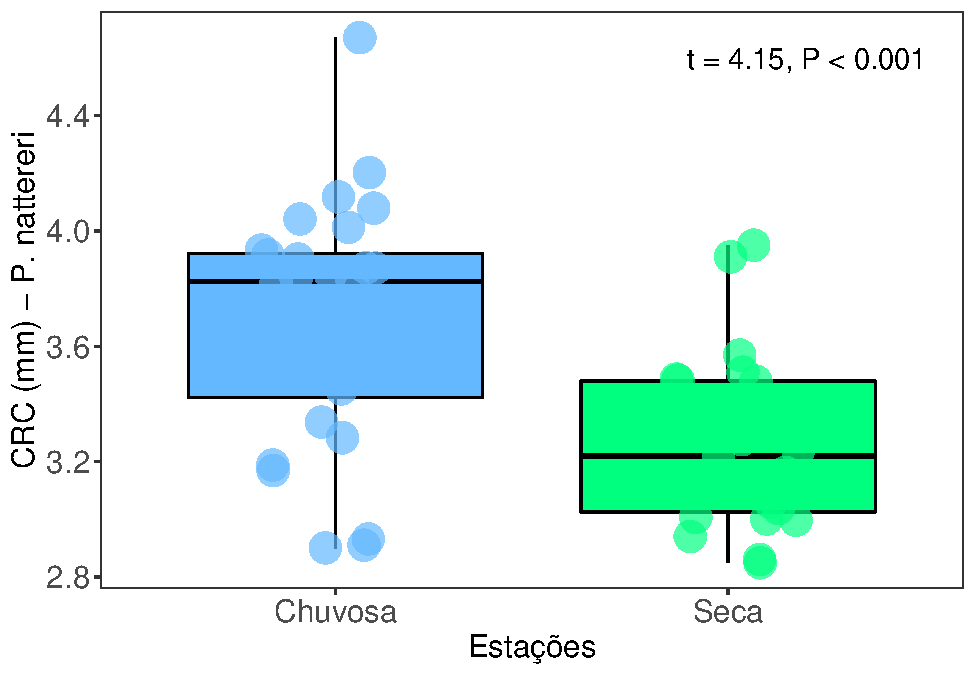
\includegraphics{livro_r_ecologia_files/figure-latex/unnamed-chunk-2-1.pdf}

\textbf{Interpretação dos resultados}

Neste exemplo, rejeitamos a hipótese nula que as médias do CRC dos machos entre as estações seca e chuvosa são iguais (t = 4,15, P \textless{} 0,001). Os resultados mostram que os machos de \emph{P. nattereri} coletados na estação chuvosa foram em média 0,43mm maiores do que os coletados na estação seca.

~

\hypertarget{exemplo-pruxe1tico-2---teste-t-para-duas-amostras-independentes-com-variuxe2ncias-diferentes}{%
\subsubsection{Exemplo prático 2 - Teste T para duas amostras independentes com variâncias diferentes}\label{exemplo-pruxe1tico-2---teste-t-para-duas-amostras-independentes-com-variuxe2ncias-diferentes}}

\hypertarget{explicauxe7uxe3o-dos-dados-1}{%
\paragraph{Explicação dos dados}\label{explicauxe7uxe3o-dos-dados-1}}

Neste exemplo, avaliaremos o comprimento rostro-cloacal (CRC - milímetros) de fêmeas de \emph{Leptodactylus podicipinus} amostradas em diferentes estações do ano com armadilhas de interceptação e queda na região noroeste do estado de São Paulo (da Silva \& Rossa-Feres 2010). \textbf{Observação:} Os dados foram alterados em relação a publicação original para se enquadrarem no exemplo de amostras com variâncias diferentes.

\textbf{Pergunta:}

\begin{quote}
O CRC das fêmeas de \emph{L. podicipinus} é maior na estação chuvosa do que na estação seca?
\end{quote}

\textbf{Predições}

\begin{quote}
O CRC das fêmeas será maior na estação chuvosa porque há uma vantangem seletiva para os indivíduos maiores durante a atividade reprodutiva.
\end{quote}

\textbf{Variáveis}

\begin{itemize}
\tightlist
\item
  Variáveis preditoras

  \begin{itemize}
  \tightlist
  \item
    Dataframe com os indivíduos (unidade amostral) nas linhas e CRC (mm - variável resposta contínua) e estação (variável preditora categórica) como colunas.
  \end{itemize}
\end{itemize}

\textbf{Checklist}

\begin{itemize}
\tightlist
\item
  Verificar se o seu dataframe está com as unidades amostrais nas linhas e variáveis preditores nas colunas
\end{itemize}

\hypertarget{anuxe1lise-1}{%
\subsection{Análise}\label{anuxe1lise-1}}

Calculo do Teste T para duas amostras com variâncias diferentes

\begin{Shaded}
\begin{Highlighting}[]
\CommentTok{## IMPORTANDO OS DADOS}
\CommentTok{#*************************}
\NormalTok{CRC_LP_femea <-}\StringTok{ }\NormalTok{ecodados}\OperatorTok{::}\NormalTok{teste_t_var_diferente}
\KeywordTok{head}\NormalTok{(CRC_LP_femea) }\CommentTok{# verificar se o dataframe foi lido corretamente}
\end{Highlighting}
\end{Shaded}

\begin{verbatim}
##    CRC Estacao
## 1 2.72 Chuvosa
## 2 2.10 Chuvosa
## 3 3.42 Chuvosa
## 4 1.50 Chuvosa
## 5 3.90 Chuvosa
## 6 4.00 Chuvosa
\end{verbatim}

\begin{Shaded}
\begin{Highlighting}[]
\CommentTok{# TESTE NORMALIDADE}
\CommentTok{#************************}
\CommentTok{## Verificando normalidade usando QQ-plot}
\CommentTok{## Os pontos não podem fugir da reta criando formas como U}
\NormalTok{residuos_LP <-}\StringTok{ }\KeywordTok{lm}\NormalTok{(CRC }\OperatorTok{~}\StringTok{ }\NormalTok{Estacao, }\DataTypeTok{data =}\NormalTok{ CRC_LP_femea)}
\KeywordTok{library}\NormalTok{(}\StringTok{"car"}\NormalTok{)}
\KeywordTok{qqPlot}\NormalTok{(residuos_LP)}
\end{Highlighting}
\end{Shaded}

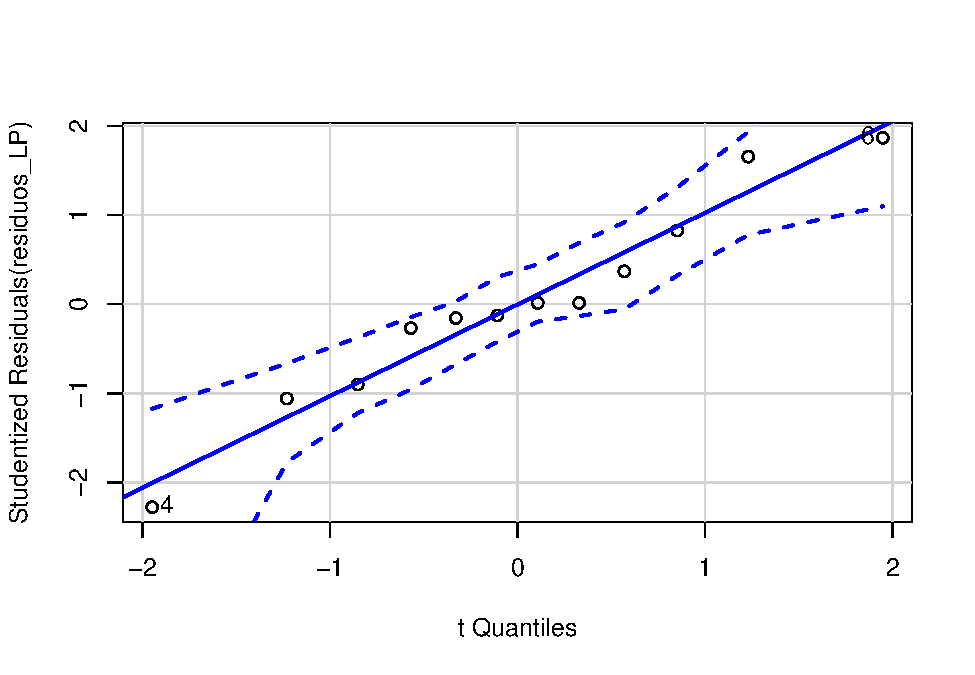
\includegraphics{livro_r_ecologia_files/figure-latex/unnamed-chunk-3-1.pdf}

\begin{verbatim}
## [1] 4 6
\end{verbatim}

\begin{Shaded}
\begin{Highlighting}[]
\CommentTok{## Outra possibilidade é usar o teste de Shapiro-Wilk para verificar normalidade}
\CommentTok{## Hipótese nula que a distribuição é normal }
\CommentTok{## valor de p < 0.05 significa que os dados não apresentam distribuição normal}
\CommentTok{## valor de p > 0.05 significa que os dados apresentam distribuição normal}
\KeywordTok{shapiro.test}\NormalTok{ (CRC_LP_femea}\OperatorTok{$}\NormalTok{CRC) }
\end{Highlighting}
\end{Shaded}

\begin{verbatim}
## 
## 	Shapiro-Wilk normality test
## 
## data:  CRC_LP_femea$CRC
## W = 0.88195, p-value = 0.09284
\end{verbatim}

\begin{Shaded}
\begin{Highlighting}[]
\CommentTok{# TESTE DE HOMOGENEIDADE DA VARIÂNCIA}
\CommentTok{#***************************************}
\CommentTok{## Hipótese nula que a variância é homogênea}
\CommentTok{## valor de p < 0.05 significa que os dados não apresentam homogeneidade}
\CommentTok{## valor de p > 0.05 significa que os dados apresentam homogeneidade}
\KeywordTok{library}\NormalTok{(car)}
\KeywordTok{leveneTest}\NormalTok{(CRC }\OperatorTok{~}\StringTok{ }\NormalTok{Estacao, }\DataTypeTok{data =}\NormalTok{ CRC_LP_femea)}
\end{Highlighting}
\end{Shaded}

\begin{verbatim}
## Levene's Test for Homogeneity of Variance (center = median)
##       Df F value  Pr(>F)  
## group  1  9.8527 0.01053 *
##       10                  
## ---
## Signif. codes:  0 '***' 0.001 '**' 0.01 '*' 0.05 '.' 0.1 ' ' 1
\end{verbatim}

\begin{Shaded}
\begin{Highlighting}[]
\CommentTok{# TESTE T COM AMOSTRAS INDEPENDENTES E VARIÂNCIS DIFERENTES}
\CommentTok{#***********************************************************}
\CommentTok{## Com base no teste de Levene, avise na linha de comando que as variâncias }
\CommentTok{## não são iguais (var.equal = FALSE).}
\KeywordTok{t.test}\NormalTok{(CRC }\OperatorTok{~}\StringTok{ }\NormalTok{Estacao, }\DataTypeTok{data =}\NormalTok{ CRC_LP_femea, }\DataTypeTok{var.equal =} \OtherTok{FALSE}\NormalTok{)}
\end{Highlighting}
\end{Shaded}

\begin{verbatim}
## 
## 	Welch Two Sample t-test
## 
## data:  CRC by Estacao
## t = -1.7633, df = 6.4998, p-value = 0.1245
## alternative hypothesis: true difference in means is not equal to 0
## 95 percent confidence interval:
##  -1.5489301  0.2375016
## sample estimates:
## mean in group Chuvosa    mean in group Seca 
##              2.834286              3.490000
\end{verbatim}

Visualizar os resultados em gráfico

\begin{Shaded}
\begin{Highlighting}[]
\KeywordTok{library}\NormalTok{(ggplot2)}
\KeywordTok{ggplot}\NormalTok{(}\DataTypeTok{data =}\NormalTok{ CRC_LP_femea, }\KeywordTok{aes}\NormalTok{(}\DataTypeTok{x=}\NormalTok{ Estacao, }\DataTypeTok{y=}\NormalTok{ CRC, }\DataTypeTok{color =}\NormalTok{ Estacao)) }\OperatorTok{+}\StringTok{ }
\StringTok{  }\KeywordTok{labs}\NormalTok{(}\DataTypeTok{x =} \StringTok{"Estações"}\NormalTok{, }\DataTypeTok{y =} \StringTok{"CRC (mm) - L. podicipinus"}\NormalTok{, }\DataTypeTok{size =} \DecValTok{15}\NormalTok{) }\OperatorTok{+}
\StringTok{  }\KeywordTok{geom_boxplot}\NormalTok{(}\DataTypeTok{fill=}\KeywordTok{c}\NormalTok{(}\StringTok{"steelblue1"}\NormalTok{, }\StringTok{"springgreen1"}\NormalTok{), }\DataTypeTok{color=}\StringTok{"black"}\NormalTok{, }\DataTypeTok{outlier.shape =} \OtherTok{NA}\NormalTok{) }\OperatorTok{+}
\StringTok{  }\KeywordTok{geom_jitter}\NormalTok{(}\DataTypeTok{shape =} \DecValTok{16}\NormalTok{, }\DataTypeTok{position=}\KeywordTok{position_jitter}\NormalTok{(}\FloatTok{0.2}\NormalTok{), }\DataTypeTok{cex =} \DecValTok{7}\NormalTok{, }\DataTypeTok{alpha =} \FloatTok{0.7}\NormalTok{) }\OperatorTok{+}
\StringTok{  }\KeywordTok{scale_color_manual}\NormalTok{(}\DataTypeTok{values =} \KeywordTok{c}\NormalTok{(}\StringTok{"steelblue1"}\NormalTok{, }\StringTok{"springgreen1"}\NormalTok{)) }\OperatorTok{+}
\StringTok{  }\KeywordTok{geom_text}\NormalTok{(}\DataTypeTok{x =} \FloatTok{2.2}\NormalTok{, }\DataTypeTok{y =} \FloatTok{1.7}\NormalTok{, }\DataTypeTok{label =} \StringTok{"t = 1.76, P = 0.12"}\NormalTok{, }\DataTypeTok{color =} \StringTok{"black"}\NormalTok{, }\DataTypeTok{size =} \DecValTok{5}\NormalTok{) }\OperatorTok{+}
\StringTok{  }\KeywordTok{theme_bw}\NormalTok{() }\OperatorTok{+}
\StringTok{  }\KeywordTok{theme}\NormalTok{(}\DataTypeTok{axis.text.y =} \KeywordTok{element_text}\NormalTok{(}\DataTypeTok{size =} \DecValTok{15}\NormalTok{), }\DataTypeTok{axis.text.x =} \KeywordTok{element_text}\NormalTok{(}\DataTypeTok{size =} \DecValTok{15}\NormalTok{)) }\OperatorTok{+}
\StringTok{  }\KeywordTok{theme}\NormalTok{(}\DataTypeTok{axis.title.y =} \KeywordTok{element_text}\NormalTok{(}\DataTypeTok{size =} \DecValTok{15}\NormalTok{), }\DataTypeTok{axis.title.x =} \KeywordTok{element_text}\NormalTok{(}\DataTypeTok{size =} \DecValTok{15}\NormalTok{)) }\OperatorTok{+}
\StringTok{  }\KeywordTok{theme}\NormalTok{(}\DataTypeTok{panel.grid.major =} \KeywordTok{element_blank}\NormalTok{(), }\DataTypeTok{panel.grid.minor =} \KeywordTok{element_blank}\NormalTok{()) }\OperatorTok{+}
\StringTok{  }\KeywordTok{theme}\NormalTok{(}\DataTypeTok{legend.position =} \StringTok{"none"}\NormalTok{)}
\end{Highlighting}
\end{Shaded}

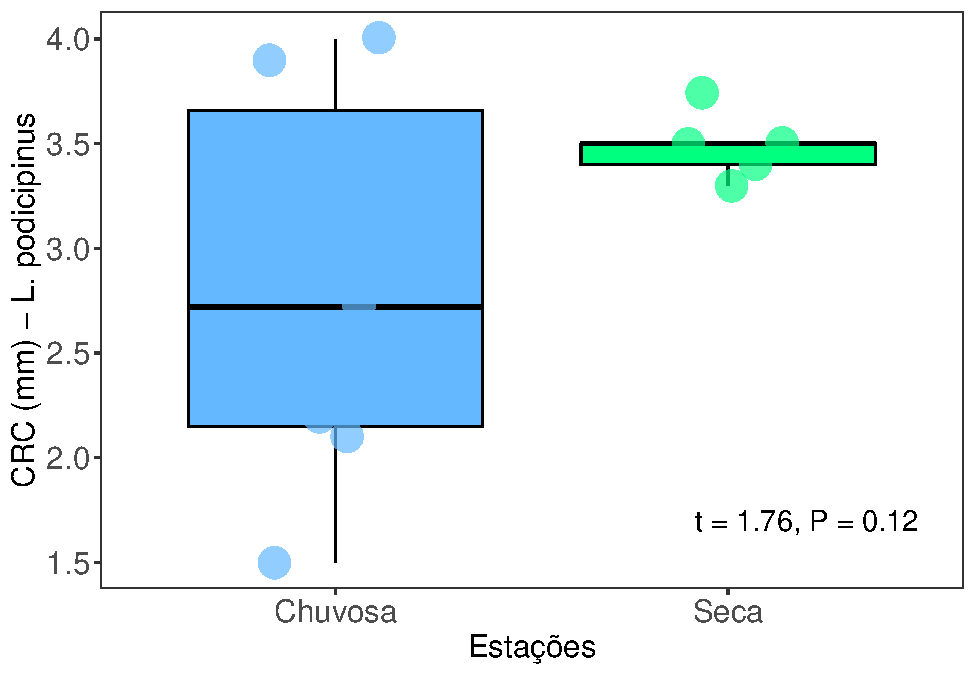
\includegraphics{livro_r_ecologia_files/figure-latex/unnamed-chunk-4-1.pdf}

\textbf{Interpretação dos resultados}

Neste exemplo, não rejeitamos a hipótese nula e consideramos que as médias do CRC das fêmeas entre as estações seca e chuvosa são iguais (t = 1,76, P = 0,12). Os resultados mostram que as fêmeas de \emph{L. podicipinus} coletadas na estação chuvosa não são maiores do que as fêmeas coletadas na estação seca.

~

\hypertarget{teste-t-para-amostras-pareadas}{%
\section{Teste T para amostras pareadas}\label{teste-t-para-amostras-pareadas}}

\hypertarget{backgorund-da-anuxe1lise-1}{%
\subsection{Backgorund da análise}\label{backgorund-da-anuxe1lise-1}}

O Teste T Pareado é uma estatística que usa dados medidos duas vezes na mesma unidade amostral, resultando em pares de observações para cada amostra (amostras pareadas). Ele determina se a diferença da média entre duas observações é zero.

\begin{quote}
\[ t = \frac{\bar{d}}{S_{\bar{d}}}\]
\end{quote}

Onde:

\begin{itemize}
\item
  \(\bar{d}\) = média da diferença das medidas pareadas. Observe que o teste não usa as medidas originais, e sim, a diferença para cada par,
\item
  S\(\bar{d}\) = erro padrão da diferença das medidas pareadas.
\end{itemize}

\begin{quote}
\hypertarget{premissas-do-teste-t-para-amostras-pareadas}{%
\subsubsection{Premissas do Teste t para amostras pareadas:}\label{premissas-do-teste-t-para-amostras-pareadas}}

\begin{itemize}
\tightlist
\item
  As unidades amostrais são selecionadas aleatoriamente;
\item
  Distribuição normal (gaussiana) dos valores da diferença para cada par;
\end{itemize}
\end{quote}

~

\hypertarget{exemplo-pruxe1tico-1---teste-t-para-amostras-pareadas}{%
\subsubsection{Exemplo prático 1 - Teste T para amostras pareadas}\label{exemplo-pruxe1tico-1---teste-t-para-amostras-pareadas}}

\hypertarget{explicauxe7uxe3o-dos-dados-2}{%
\paragraph{Explicação dos dados}\label{explicauxe7uxe3o-dos-dados-2}}

Neste exemplo avaliaremos a diferença na riqueza de espécies de artrópodes registradas em 27 localidades. Todas as localidades foram amostradas duas vezes. A primeira amostragem foi realizada com na localidade antes da pertubação e a segunda amostragem foi realizada após a localidade ter sofrido uma queimada.

\textbf{Pergunta:}

\begin{quote}
A riqueza de espécies de artrópodes é prejudicada pelas queimadas?
\end{quote}

\textbf{Predições}

\begin{quote}
A riqueza de espécies de artrópodes será maior antes da queimada devido a extinção local das espécies.
\end{quote}

\textbf{Variáveis}

\begin{itemize}
\tightlist
\item
  Variáveis preditoras

  \begin{itemize}
  \tightlist
  \item
    Dataframe com as localidades nas linhas e riqueza de espécies (variável preditora contínua) e estado (Pre-queimada ou Pós-queimada - variável categórica) da localidade nas colunas.
  \end{itemize}
\end{itemize}

\textbf{Checklist}

\begin{itemize}
\tightlist
\item
  Verificar se o seu dataframe está com as unidades amostrais nas linhas e variáveis preditores nas colunas
\end{itemize}

\hypertarget{anuxe1lise-2}{%
\subsection{Análise}\label{anuxe1lise-2}}

Calculo do Teste T com amostras pareadas

\begin{Shaded}
\begin{Highlighting}[]
\CommentTok{## IMPORTANDO OS DADOS}
\CommentTok{#*************************}
\NormalTok{Pareado <-}\StringTok{ }\NormalTok{ecodados}\OperatorTok{::}\NormalTok{teste_t_pareado}
\KeywordTok{head}\NormalTok{(Pareado) }\CommentTok{# verificar se o dataframe foi lido corretamente}
\end{Highlighting}
\end{Shaded}

\begin{verbatim}
##   Areas Riqueza       Estado
## 1     1      92 Pre-Queimada
## 2     2      74 Pre-Queimada
## 3     3      96 Pre-Queimada
## 4     4      89 Pre-Queimada
## 5     5      76 Pre-Queimada
## 6     6      80 Pre-Queimada
\end{verbatim}

\begin{Shaded}
\begin{Highlighting}[]
\CommentTok{# TESTE T PAREADO}
\CommentTok{#*****************}
\CommentTok{# O uso do [] é para selecionar dentro do vetor/coluna *Riqueza* os 27 primeiros números [1:27] que representam as localidades antes da queimada e os últimos 27 números [28:54] que representam as mesmas localidades pós-queimada}
\KeywordTok{t.test}\NormalTok{(Pareado}\OperatorTok{$}\NormalTok{Riqueza[}\DecValTok{1}\OperatorTok{:}\DecValTok{27}\NormalTok{], Pareado}\OperatorTok{$}\NormalTok{Riqueza[}\DecValTok{28}\OperatorTok{:}\DecValTok{54}\NormalTok{], }\DataTypeTok{paired =} \OtherTok{TRUE}\NormalTok{)}
\end{Highlighting}
\end{Shaded}

\begin{verbatim}
## 
## 	Paired t-test
## 
## data:  Pareado$Riqueza[1:27] and Pareado$Riqueza[28:54]
## t = 7.5788, df = 26, p-value = 4.803e-08
## alternative hypothesis: true difference in means is not equal to 0
## 95 percent confidence interval:
##  32.47117 56.63994
## sample estimates:
## mean of the differences 
##                44.55556
\end{verbatim}

Visualizar os resultados em gráfico

\begin{Shaded}
\begin{Highlighting}[]
\KeywordTok{library}\NormalTok{(}\StringTok{"ggpubr"}\NormalTok{)}
\KeywordTok{ggpaired}\NormalTok{(Pareado, }\DataTypeTok{x =} \StringTok{"Estado"}\NormalTok{, }\DataTypeTok{y =} \StringTok{"Riqueza"}\NormalTok{,}
         \DataTypeTok{color =} \StringTok{"Estado"}\NormalTok{, }\DataTypeTok{line.color =} \StringTok{"gray"}\NormalTok{, }\DataTypeTok{line.size =} \FloatTok{0.8}\NormalTok{, }\DataTypeTok{palette =} \StringTok{"jco"}\NormalTok{, }\DataTypeTok{width =} \FloatTok{0.8}\NormalTok{,}
         \DataTypeTok{point.size =} \DecValTok{3}\NormalTok{, }\DataTypeTok{xlab =} \StringTok{"Estado das localidades"}\NormalTok{, }\DataTypeTok{ylab =} \StringTok{"Riqueza de Espécies"}\NormalTok{) }\OperatorTok{+}
\StringTok{  }\KeywordTok{expand_limits}\NormalTok{(}\DataTypeTok{y=}\KeywordTok{c}\NormalTok{(}\DecValTok{0}\NormalTok{,}\DecValTok{150}\NormalTok{)) }
\end{Highlighting}
\end{Shaded}

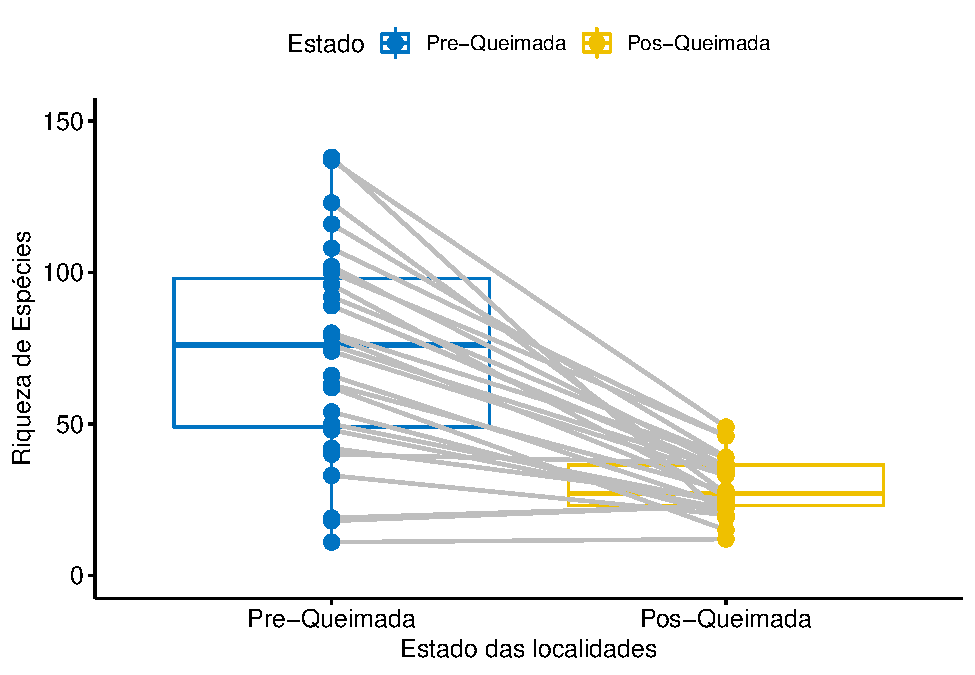
\includegraphics{livro_r_ecologia_files/figure-latex/unnamed-chunk-6-1.pdf}

\textbf{Interpretação dos resultados}

Neste exemplo, rejeitamos a hipótese nula que a riqueza de espécies de artrópodes é igual antes e depois da queimada (t = 7,57, P \textless{} 0,001). Os resultados mostram que as localidades após as queimadas apresentam em média 44,5 espécies de artrópodes a menos do que antes das queimadas.

~

\hypertarget{correlauxe7uxe3o-de-pearson}{%
\section{Correlação de Pearson}\label{correlauxe7uxe3o-de-pearson}}

\hypertarget{backgorund-da-anuxe1lise-2}{%
\subsection{Backgorund da análise}\label{backgorund-da-anuxe1lise-2}}

É um teste que mede a força relativa da relação linear entre duas variáveis contínuas (X e Y). Importante ressaltar que a análise de correlação não assume que a variável X influêncie a variável Y ou que exista uma relação de causa e efeito entre elas (Zar 2016). A análise é definida em termos da variância de X, a variância de Y, e a covariância de X e Y (i.e.~como elas variam juntas).

\begin{quote}
\[ r = \frac{\sum{XY} - \frac{\sum{X} \sum{Y}}{n}}{\sqrt{\left(\sum{X^2} - \frac{\sum{X}^2}{n}\right)\left(\sum{Y^2} - \frac{\sum{Y}^2}{n}\right)}} \]
\end{quote}

Onde:

\begin{itemize}
\tightlist
\item
  r = coeficiente de correlação que indica a força da relação entre as duas variáveis. Seu range de valores está entre -1 \(\leq\) r \(\geq\) 1. A correlação positiva indica que o aumento no valor de uma das variáveis é acompanhado pelo aumento no valor da outra variável. A correlação negativa indica que um aumento no valor de uma das variáveis é acompanhado pela diminuição no valor da outra variável. Se \emph{r} é igual a zero, não existe correlação entre as variáveis.
\end{itemize}

\begin{quote}
\hypertarget{premissas-da-correlauxe7uxe3o-de-person}{%
\subsubsection{Premissas da Correlação de Person:}\label{premissas-da-correlauxe7uxe3o-de-person}}

\begin{itemize}
\tightlist
\item
  As amostras devem ser independentes e pareadas (i.e.~as duas variáveis devem ser medidas na mesma unidade amostral);
\item
  As unidades amostrais são selecionadas aleatoriamente;
\item
  A relação entre as variáveis tem que ser linear.
\end{itemize}
\end{quote}

~

\hypertarget{exemplo-pruxe1tico-1---correlauxe7uxe3o-de-pearson}{%
\subsubsection{Exemplo prático 1 - Correlação de Pearson}\label{exemplo-pruxe1tico-1---correlauxe7uxe3o-de-pearson}}

\hypertarget{explicauxe7uxe3o-dos-dados-3}{%
\paragraph{Explicação dos dados}\label{explicauxe7uxe3o-dos-dados-3}}

Neste exemplo avaliaremos a correlação entre a altura do tronco e o tamanho da raiz medidos em 35 indivíduos de uma espécie vegetal arbustiva.

\textbf{Pergunta:}

\begin{quote}
Existe correlação entre a altura do tronco e o tamanho da raiz dos arbustos?
\end{quote}

\textbf{Predições}

\begin{quote}
A altura do tronco é positivamente correlacionado com o tamanho da raiz.
\end{quote}

\textbf{Variáveis}

\begin{itemize}
\tightlist
\item
  Variáveis preditoras

  \begin{itemize}
  \tightlist
  \item
    Dataframe com os indivíduos (unidade amostral) nas linhas e altura do tronco e tamanho da raiz (duas variáveis tem que ser contínuas) como colunas.
  \end{itemize}
\end{itemize}

\textbf{Checklist}

\begin{itemize}
\tightlist
\item
  Verificar se o seu dataframe está com as unidades amostrais nas linhas e variáveis preditores nas colunas
\end{itemize}

\hypertarget{anuxe1lise-3}{%
\subsection{Análise}\label{anuxe1lise-3}}

Calculo do Teste de Correlação de Pearson

\begin{Shaded}
\begin{Highlighting}[]
\CommentTok{## IMPORTANDO OS DADOS}
\CommentTok{#************************}
\NormalTok{correlacao_arbustos <-}\StringTok{ }\NormalTok{ecodados}\OperatorTok{::}\NormalTok{correlacao}
\KeywordTok{head}\NormalTok{(correlacao_arbustos) }\CommentTok{# verificar se o dataframe foi lido corretamente}
\end{Highlighting}
\end{Shaded}

\begin{verbatim}
##   Tamanho_raiz Tamanho_tronco
## 1    10.177049       19.54383
## 2     6.622634       17.13558
## 3     7.773629       19.50681
## 4    11.055257       21.57085
## 5     4.487274       13.22763
## 6    11.190216       21.62902
\end{verbatim}

\begin{Shaded}
\begin{Highlighting}[]
\CommentTok{# Teste de Correlação de Pearson}
\CommentTok{#********************************}
\CommentTok{# Para outros testes de correlação como Kendall ou Spearman é só alterar na linha de comando a opção *method* e inserir o teste desejado.}
\KeywordTok{cor.test}\NormalTok{(correlacao_arbustos}\OperatorTok{$}\NormalTok{Tamanho_raiz, correlacao_arbustos}\OperatorTok{$}\NormalTok{Tamanho_tronco, }\DataTypeTok{method =} \StringTok{"pearson"}\NormalTok{)}
\end{Highlighting}
\end{Shaded}

\begin{verbatim}
## 
## 	Pearson's product-moment correlation
## 
## data:  correlacao_arbustos$Tamanho_raiz and correlacao_arbustos$Tamanho_tronco
## t = 11.49, df = 33, p-value = 4.474e-13
## alternative hypothesis: true correlation is not equal to 0
## 95 percent confidence interval:
##  0.7995083 0.9457816
## sample estimates:
##       cor 
## 0.8944449
\end{verbatim}

Visualizar os resultados em gráfico

\begin{Shaded}
\begin{Highlighting}[]
\KeywordTok{library}\NormalTok{(ggplot2)}
\KeywordTok{ggplot}\NormalTok{(}\DataTypeTok{data =}\NormalTok{ correlacao_arbustos, }\KeywordTok{aes}\NormalTok{(}\DataTypeTok{x=}\NormalTok{ Tamanho_raiz, }\DataTypeTok{y=}\NormalTok{ Tamanho_tronco)) }\OperatorTok{+}\StringTok{ }
\StringTok{  }\KeywordTok{labs}\NormalTok{(}\DataTypeTok{x =} \StringTok{"Tamanho da raiz"}\NormalTok{, }\DataTypeTok{y =} \StringTok{"Altura do tronco"}\NormalTok{, }\DataTypeTok{size =} \DecValTok{20}\NormalTok{) }\OperatorTok{+}
\StringTok{  }\KeywordTok{geom_point}\NormalTok{(}\DataTypeTok{size =} \DecValTok{15}\NormalTok{, }\DataTypeTok{shape =} \DecValTok{21}\NormalTok{, }\DataTypeTok{fill =} \StringTok{"gray"}\NormalTok{) }\OperatorTok{+}
\StringTok{  }\KeywordTok{geom_text}\NormalTok{(}\DataTypeTok{x =} \DecValTok{14}\NormalTok{, }\DataTypeTok{y =} \DecValTok{14}\NormalTok{, }\DataTypeTok{label =} \StringTok{"r = 0.89, P < 0.001"}\NormalTok{, }\DataTypeTok{color =} \StringTok{"black"}\NormalTok{, }\DataTypeTok{size =} \DecValTok{7}\NormalTok{) }\OperatorTok{+}
\StringTok{  }\KeywordTok{theme_bw}\NormalTok{() }\OperatorTok{+}
\StringTok{  }\KeywordTok{theme}\NormalTok{(}\DataTypeTok{axis.title.y =} \KeywordTok{element_text}\NormalTok{(}\DataTypeTok{size =} \DecValTok{20}\NormalTok{), }\DataTypeTok{axis.title.x =} \KeywordTok{element_text}\NormalTok{(}\DataTypeTok{size =} \DecValTok{20}\NormalTok{)) }\OperatorTok{+}
\StringTok{  }\KeywordTok{theme}\NormalTok{(}\DataTypeTok{axis.text.y =} \KeywordTok{element_text}\NormalTok{(}\DataTypeTok{size =} \DecValTok{20}\NormalTok{), }\DataTypeTok{axis.text.x =} \KeywordTok{element_text}\NormalTok{(}\DataTypeTok{size =} \DecValTok{20}\NormalTok{)) }\OperatorTok{+}
\StringTok{  }\KeywordTok{theme}\NormalTok{(}\DataTypeTok{panel.grid.major =} \KeywordTok{element_blank}\NormalTok{(), }\DataTypeTok{panel.grid.minor =} \KeywordTok{element_blank}\NormalTok{(), }
        \DataTypeTok{panel.border =} \KeywordTok{element_rect}\NormalTok{(}\DataTypeTok{colour =} \StringTok{"black"}\NormalTok{, }\DataTypeTok{fill=}\OtherTok{NA}\NormalTok{, }\DataTypeTok{size =} \DecValTok{2}\NormalTok{)) }\OperatorTok{+}
\StringTok{  }\KeywordTok{geom_smooth}\NormalTok{(}\DataTypeTok{method =}\NormalTok{ lm, }\DataTypeTok{se =} \OtherTok{FALSE}\NormalTok{, }\DataTypeTok{color =} \StringTok{"black"}\NormalTok{, }\DataTypeTok{linetype=}\StringTok{"dashed"}\NormalTok{) }
\end{Highlighting}
\end{Shaded}

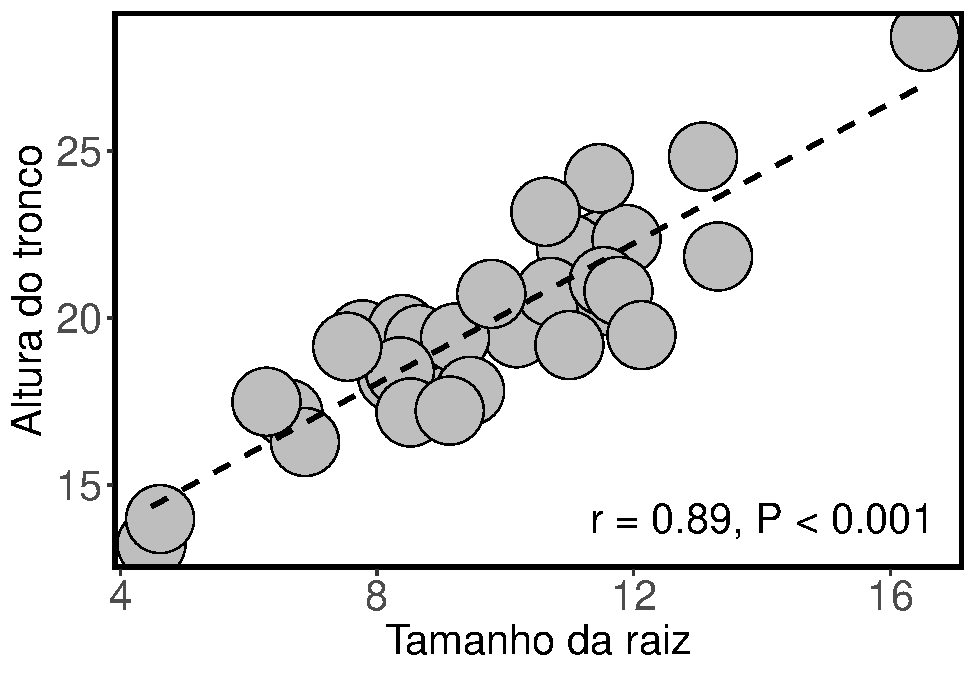
\includegraphics{livro_r_ecologia_files/figure-latex/unnamed-chunk-8-1.pdf}

\textbf{Interpretação dos resultados}

Neste exemplo, rejeitamos a hipótese nula que as variáveis não são correlacionadas (r = 0.89, P \textless{} 0,001). Os resultados mostram que o aumento na altura dos arbutos é acompanhado pelo aumento no tamanho da raiz.

~

\hypertarget{regressuxe3o-simples}{%
\section{Regressão Simples}\label{regressuxe3o-simples}}

\hypertarget{backgorund-da-anuxe1lise-3}{%
\subsection{Backgorund da análise}\label{backgorund-da-anuxe1lise-3}}

A regressão simples é usada para analisar a relação entre uma variável preditora (plotada no eixo-X) e uma variável resposta (plotada no eixo-Y). As duas variáveis devem ser contínuas. Diferente das correlações, a regressão assume uma relação de causa e efeito entre as variáveis. O valor da variável preditora (X) causa, direta ou indiretamente, o valor da variável resposta (Y). Assim, Y é uma função linear de X:

\begin{quote}
\[ Y = \beta_0 + \beta_{1}X_i + \epsilon_i \]
\end{quote}

Onde:

\begin{itemize}
\item
  \(\beta_0\) = intercepto que representa o valor da função quando X = 0,
\item
  \(\beta_{1}\) = inclinação (\emph{slope}) que mede a mudança na variável Y para cada mudança de unidade da variável X.
\item
  \(\epsilon_{1}\) = erro aleatório referente a variável Y que não pode ser explicado pela variável X.
\end{itemize}

\begin{quote}
\hypertarget{premissas-da-regressuxe3o-simples}{%
\subsubsection{Premissas da Regressão Simples:}\label{premissas-da-regressuxe3o-simples}}

\begin{itemize}
\tightlist
\item
  As amostras devem ser independentes;
\item
  As unidades amostrais são selecionadas aleatoriamente;
\item
  Distribuição normal (gaussiana) dos resíduos;
\item
  Homogeneidade da variância.
\end{itemize}
\end{quote}

~

\hypertarget{exemplo-pruxe1tico-1---regressuxe3o-simples}{%
\subsubsection{Exemplo prático 1 - Regressão simples}\label{exemplo-pruxe1tico-1---regressuxe3o-simples}}

\hypertarget{explicauxe7uxe3o-dos-dados-4}{%
\paragraph{Explicação dos dados}\label{explicauxe7uxe3o-dos-dados-4}}

Neste exemplo, avaliaremos a relação entre o gradiente de temperatura média anual (°C) e o tamanho médio do comprimento rostro-cloacal (CRC em mm) de populações de \emph{Dendropsophus minutus} (Anura:Hylidae) amostradas em 109 localidades no Brasil (Boaratti \& da Silva 2015).

\textbf{Pergunta:}

\begin{quote}
Há relação entre o tamanho do CRC das populações e a temperatura das localidades onde os indivíduos ocorrem?
\end{quote}

\textbf{Predições}

\begin{quote}
O CRC das populações serão menores em localidades mais quentes do que em localidades mais frias de acordo com a Hipótese do balanço de calor.
\end{quote}

\textbf{Variáveis}

\begin{itemize}
\tightlist
\item
  Variáveis preditoras

  \begin{itemize}
  \tightlist
  \item
    Dataframe com as populações (unidade amostral) nas linhas e CRC médio (mm) e temperatura média anual como colunas.
  \end{itemize}
\end{itemize}

\textbf{Checklist}

\begin{itemize}
\tightlist
\item
  Verificar se o seu dataframe está com as unidades amostrais nas linhas e variáveis preditores nas colunas
\end{itemize}

\hypertarget{anuxe1lise-4}{%
\subsection{Análise}\label{anuxe1lise-4}}

Calculo da regressão simples

\begin{Shaded}
\begin{Highlighting}[]
\CommentTok{## IMPORTANDO DADOS}
\CommentTok{#********************}
\NormalTok{dados_regressao <-}\StringTok{ }\NormalTok{ecodados}\OperatorTok{::}\NormalTok{regressoes}
\KeywordTok{head}\NormalTok{(dados_regressao) }\CommentTok{# verificar se o dataframe foi lido corretamente}
\end{Highlighting}
\end{Shaded}

\begin{verbatim}
##      Municipio      CRC Temperatura Precipitacao
## 1     Acorizal 22.98816    24.13000       1228.2
## 2  Alpinopolis 22.91788    20.09417       1487.6
## 3 Alto_Paraiso 21.97629    21.86167       1812.4
## 4    Americana 23.32453    20.28333       1266.2
## 5      Apiacas 22.83651    25.47333       2154.0
## 6  Arianopolis 20.86989    20.12167       1269.2
\end{verbatim}

\begin{Shaded}
\begin{Highlighting}[]
\CommentTok{# ANALISE DA REGRESSÃO}
\CommentTok{#************************}
\NormalTok{modelo_regressao <-}\StringTok{ }\KeywordTok{lm}\NormalTok{(CRC }\OperatorTok{~}\StringTok{ }\NormalTok{Temperatura, }\DataTypeTok{data =}\NormalTok{ dados_regressao)}

\CommentTok{# PRIMEIRO VAMOS VERIFICAR A NORMALIDADE E HOMOGENEIDADE DAS VARIÂNCIAS}
\CommentTok{#***********************************************************************}
\CommentTok{# Os gráficos *Residuals vs Fitted*, *Scale-Location*, e *Residual vs Leverage* estão relacionados com a homogeneidade da variância. Nestes gráficos, esperamos ver os pontos dispersos no espaço sem padrões com formatos em *U* ou funil. }
\CommentTok{# O gráfico *Normal Q-Q* está relacionado com a distribuição normal dos resíduos. Neste gráfico, esperamos ver os pontos próximos a reta sem padrões com formatos em *U* ou *S*. }
\KeywordTok{par}\NormalTok{(}\DataTypeTok{mfrow =} \KeywordTok{c}\NormalTok{(}\DecValTok{2}\NormalTok{, }\DecValTok{2}\NormalTok{), }\DataTypeTok{oma =} \KeywordTok{c}\NormalTok{(}\DecValTok{0}\NormalTok{, }\DecValTok{0}\NormalTok{, }\DecValTok{2}\NormalTok{, }\DecValTok{0}\NormalTok{))}
\KeywordTok{plot}\NormalTok{(modelo_regressao)}
\end{Highlighting}
\end{Shaded}

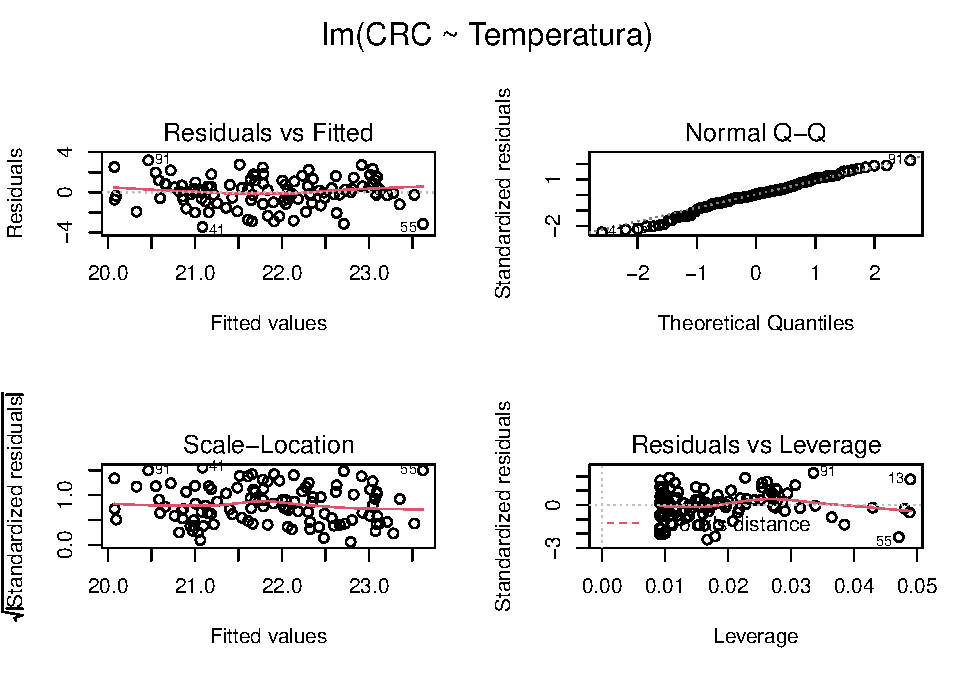
\includegraphics{livro_r_ecologia_files/figure-latex/unnamed-chunk-9-1.pdf}

\begin{Shaded}
\begin{Highlighting}[]
\KeywordTok{dev.off}\NormalTok{()}
\end{Highlighting}
\end{Shaded}

\begin{verbatim}
## null device 
##           1
\end{verbatim}

\begin{Shaded}
\begin{Highlighting}[]
\CommentTok{# VERIFICANDO OS RESULTADOS DA REGRESSÃO}
\CommentTok{#****************************************}
\KeywordTok{anova}\NormalTok{(modelo_regressao)}
\end{Highlighting}
\end{Shaded}

\begin{verbatim}
## Analysis of Variance Table
## 
## Response: CRC
##              Df  Sum Sq Mean Sq F value    Pr(>F)    
## Temperatura   1  80.931  80.931   38.92 9.011e-09 ***
## Residuals   107 222.500   2.079                      
## ---
## Signif. codes:  0 '***' 0.001 '**' 0.01 '*' 0.05 '.' 0.1 ' ' 1
\end{verbatim}

\begin{Shaded}
\begin{Highlighting}[]
\CommentTok{# ou}
\CommentTok{# esta função apresenta os resultados mais detalhados com a estimativa do intercepto, inclinação da reta (slope) e o coeficiente de determinação (R2) que indica a proporção da variação na variável Y que pode ser atribuída à variação na variável X.}
\KeywordTok{summary}\NormalTok{(modelo_regressao)}
\end{Highlighting}
\end{Shaded}

\begin{verbatim}
## 
## Call:
## lm(formula = CRC ~ Temperatura, data = dados_regressao)
## 
## Residuals:
##     Min      1Q  Median      3Q     Max 
## -3.4535 -0.7784  0.0888  0.9168  3.1868 
## 
## Coefficients:
##             Estimate Std. Error t value Pr(>|t|)    
## (Intercept) 16.23467    0.91368  17.768  < 2e-16 ***
## Temperatura  0.26905    0.04313   6.239 9.01e-09 ***
## ---
## Signif. codes:  0 '***' 0.001 '**' 0.01 '*' 0.05 '.' 0.1 ' ' 1
## 
## Residual standard error: 1.442 on 107 degrees of freedom
## Multiple R-squared:  0.2667,	Adjusted R-squared:  0.2599 
## F-statistic: 38.92 on 1 and 107 DF,  p-value: 9.011e-09
\end{verbatim}

Visualizar os resultados em gráfico

\begin{Shaded}
\begin{Highlighting}[]
\KeywordTok{library}\NormalTok{(ggplot2)}
\KeywordTok{ggplot}\NormalTok{(}\DataTypeTok{data =}\NormalTok{ dados_regressao, }\KeywordTok{aes}\NormalTok{(}\DataTypeTok{x=}\NormalTok{ Temperatura, }\DataTypeTok{y=}\NormalTok{ CRC)) }\OperatorTok{+}\StringTok{ }
\StringTok{  }\KeywordTok{labs}\NormalTok{(}\DataTypeTok{x =} \StringTok{"Temperatura média anual (°C)"}\NormalTok{, }\DataTypeTok{y =} \StringTok{"Comprimento rostro-cloacal (mm)"}\NormalTok{, }\DataTypeTok{size =} \DecValTok{20}\NormalTok{) }\OperatorTok{+}
\StringTok{  }\KeywordTok{geom_point}\NormalTok{(}\DataTypeTok{size =} \DecValTok{15}\NormalTok{, }\DataTypeTok{shape =} \DecValTok{21}\NormalTok{, }\DataTypeTok{fill =} \StringTok{"gray"}\NormalTok{) }\OperatorTok{+}
\StringTok{  }\KeywordTok{geom_text}\NormalTok{(}\DataTypeTok{x =} \DecValTok{25}\NormalTok{, }\DataTypeTok{y =} \FloatTok{17.8}\NormalTok{, }\DataTypeTok{label =} \StringTok{"R2 = 0.26, P < 0.001"}\NormalTok{, }\DataTypeTok{color =} \StringTok{"black"}\NormalTok{, }\DataTypeTok{size =} \DecValTok{7}\NormalTok{) }\OperatorTok{+}
\StringTok{  }\KeywordTok{theme_bw}\NormalTok{() }\OperatorTok{+}
\StringTok{  }\KeywordTok{theme}\NormalTok{(}\DataTypeTok{axis.title.y =} \KeywordTok{element_text}\NormalTok{(}\DataTypeTok{size =} \DecValTok{20}\NormalTok{), }\DataTypeTok{axis.title.x =} \KeywordTok{element_text}\NormalTok{(}\DataTypeTok{size =} \DecValTok{20}\NormalTok{)) }\OperatorTok{+}
\StringTok{  }\KeywordTok{theme}\NormalTok{(}\DataTypeTok{axis.text.y =} \KeywordTok{element_text}\NormalTok{(}\DataTypeTok{size =} \DecValTok{20}\NormalTok{), }\DataTypeTok{axis.text.x =} \KeywordTok{element_text}\NormalTok{(}\DataTypeTok{size =} \DecValTok{20}\NormalTok{)) }\OperatorTok{+}
\StringTok{  }\KeywordTok{theme}\NormalTok{(}\DataTypeTok{panel.grid.major =} \KeywordTok{element_blank}\NormalTok{(), }\DataTypeTok{panel.grid.minor =} \KeywordTok{element_blank}\NormalTok{(), }
        \DataTypeTok{panel.border =} \KeywordTok{element_rect}\NormalTok{(}\DataTypeTok{colour =} \StringTok{"black"}\NormalTok{, }\DataTypeTok{fill=}\OtherTok{NA}\NormalTok{, }\DataTypeTok{size =} \DecValTok{2}\NormalTok{)) }\OperatorTok{+}
\StringTok{  }\KeywordTok{geom_smooth}\NormalTok{(}\DataTypeTok{method =}\NormalTok{ lm, }\DataTypeTok{se =} \OtherTok{FALSE}\NormalTok{, }\DataTypeTok{color =} \StringTok{"black"}\NormalTok{) }
\end{Highlighting}
\end{Shaded}

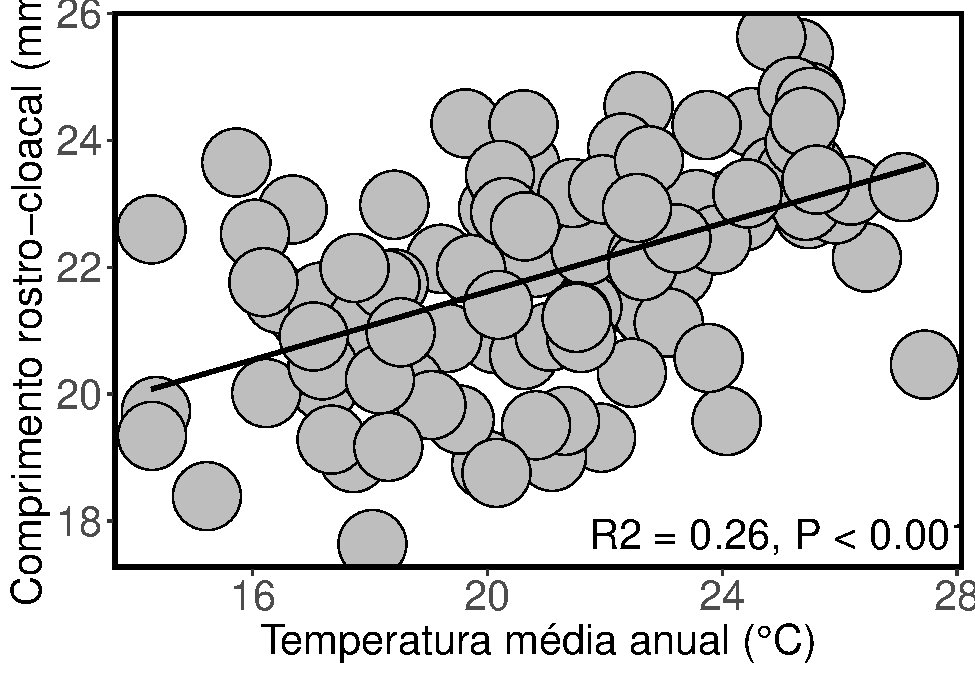
\includegraphics{livro_r_ecologia_files/figure-latex/unnamed-chunk-10-1.pdf}

\textbf{Interpretação dos resultados}

Neste exemplo, rejeitamos a hipótese nula que não existe relação entre o tamanho do CRC das populações de \emph{D. minutus} e a temperatura da localidade onde elas ocorrem (F1,107 = 38,92, P \textless{} 0,001). Os resultados mostram que o tamanho do CRC das populações tem uma relação positiva com a temperatura das localidades. Assim, populações de \emph{D. minutus} em localidades mais quentes apresentam maior CRC do que as populações em localidades mais frias.

~

\hypertarget{regressuxe3o-muxfaltipla}{%
\section{Regressão Múltipla}\label{regressuxe3o-muxfaltipla}}

\hypertarget{backgorund-da-anuxe1lise-4}{%
\subsection{Backgorund da análise}\label{backgorund-da-anuxe1lise-4}}

A regressão múltipla é uma extensão da regressão simples. Ela é usada quando queremos determinar o valor da variável resposta (Y) com base nos valores de duas ou mais variáveis preditoras (X1, X2, X\emph{n}).

\begin{quote}
\[ Y = \beta_0 + \beta_{1}X_1 + \beta_{n}X_n + \epsilon_i \]
\end{quote}

Onde:

\begin{itemize}
\item
  \(\beta_0\) = intercepto que representa o valor da função quando X = 0;
\item
  \(\beta_{n}\) = inclinação (\emph{slope}) que mede a mudança na variável Y para cada mudança de unidade das variáveis Xn;
\item
  \(\epsilon_{1}\) = erro aleatório referente a variável Y que não pode ser explicado pelas variáveis preditoras.
\end{itemize}

\begin{quote}
\hypertarget{premissas-da-regressuxe3o-muxfaltipla}{%
\subsubsection{Premissas da Regressão Múltipla:}\label{premissas-da-regressuxe3o-muxfaltipla}}

\begin{itemize}
\tightlist
\item
  As amostras devem ser independentes;
\item
  As unidades amostrais são selecionadas aleatoriamente;
\item
  Distribuição normal (gaussiana) dos resíduos;
\item
  Homogeneidade da variância.
\end{itemize}
\end{quote}

~

\hypertarget{exemplo-pruxe1tico-1---regressuxe3o-muxfaltipla}{%
\subsubsection{Exemplo prático 1 - Regressão múltipla}\label{exemplo-pruxe1tico-1---regressuxe3o-muxfaltipla}}

\hypertarget{explicauxe7uxe3o-dos-dados-5}{%
\paragraph{Explicação dos dados}\label{explicauxe7uxe3o-dos-dados-5}}

Utilizaremos o mesmo exemplo da regressão simples. Contudo, além do gradiente de temperatura média anual (°C) incluiremos o gradiente de precipitação anual (mm) como outra variável preditora do tamanho médio do comprimento rostro-cloacal (CRC em mm) de populações de \emph{Dendropsophus minutus} (Anura:Hylidae) amostradas em 109 localidades no Brasil (Boaratti \& da Silva 2015).

\textbf{Pergunta:}

\begin{quote}
O tamanho do CRC das populações de \emph{D. minutus} é influênciado pela temperatura e precipitação das localidades onde os indivíduos ocorrem?
\end{quote}

\textbf{Predições}

\begin{quote}
O CRC das populações serão menores em localidades com clima quente e chuvoso do que em localidades com clima frio e seco.
\end{quote}

\textbf{Variáveis}

\begin{itemize}
\tightlist
\item
  Variáveis preditoras

  \begin{itemize}
  \tightlist
  \item
    Dataframe com as populações (unidade amostral) nas linhas e CRC médio (mm) e temperatura e precipitação como colunas.
  \end{itemize}
\end{itemize}

\textbf{Checklist}

\begin{itemize}
\tightlist
\item
  Verificar se o seu dataframe está com as unidades amostrais nas linhas e variáveis preditores nas colunas
\end{itemize}

\hypertarget{anuxe1lise-5}{%
\subsection{Análise}\label{anuxe1lise-5}}

Cálculo da regressão múltipla

\begin{Shaded}
\begin{Highlighting}[]
\CommentTok{## IMPORTANDO DADOS}
\CommentTok{#********************}
\NormalTok{dados_regressao_mul <-}\StringTok{ }\NormalTok{ecodados}\OperatorTok{::}\NormalTok{regressoes}
\KeywordTok{head}\NormalTok{(dados_regressao_mul) }\CommentTok{# verificar se o dataframe foi lido corretamente}
\end{Highlighting}
\end{Shaded}

\begin{verbatim}
##      Municipio      CRC Temperatura Precipitacao
## 1     Acorizal 22.98816    24.13000       1228.2
## 2  Alpinopolis 22.91788    20.09417       1487.6
## 3 Alto_Paraiso 21.97629    21.86167       1812.4
## 4    Americana 23.32453    20.28333       1266.2
## 5      Apiacas 22.83651    25.47333       2154.0
## 6  Arianopolis 20.86989    20.12167       1269.2
\end{verbatim}

\begin{Shaded}
\begin{Highlighting}[]
\CommentTok{# ANALISE DA REGRESSÃO}
\CommentTok{#************************}
\NormalTok{modelo_regressao_mul <-}\StringTok{ }\KeywordTok{lm}\NormalTok{(CRC }\OperatorTok{~}\StringTok{ }\NormalTok{Temperatura }\OperatorTok{+}\StringTok{ }\NormalTok{Precipitacao, }\DataTypeTok{data =}\NormalTok{ dados_regressao_mul)}

\CommentTok{# MULTICOLINEARIDADE}
\CommentTok{#********************}
\CommentTok{# Multicolinearidade ocorre quando as variáveis preditoras são correlacionadas. Essa correlação é um problema porque as variáveis preditores deveriam ser independentes. O Fator de Inflação da Variância (VIF) é um teste que identifica a correlação entre as variáveis e mostra a força dessa correlação. Alguns autores consideram valores de VIF acima de 10 como fortemente correlacionadas, outros mais conservadores consideram o valor de 3.}
\KeywordTok{library}\NormalTok{(car)}
\KeywordTok{vif}\NormalTok{(modelo_regressao_mul)}
\end{Highlighting}
\end{Shaded}

\begin{verbatim}
##  Temperatura Precipitacao 
##     1.041265     1.041265
\end{verbatim}

\begin{Shaded}
\begin{Highlighting}[]
\CommentTok{# VERIFICANDO A NORMALIDADE E HOMOGENEIDADE DAS VARIÂNCIAS}
\CommentTok{#***********************************************************************}
\CommentTok{# Os gráficos *Residuals vs Fitted*, *Scale-Location*, e *Residual vs Leverage* estão relacionados com a homogeneidade da variância. Nestes gráficos, esperamos ver os pontos dispersos no espaço sem padrões em forma de *U* ou funil. }
\CommentTok{# O gráfico *Normal Q-Q* está relacionado com a distribuição normal dos resíduos. Neste gráfico, esperamos ver os pontos próximos a reta sem padrões em forma de *U* ou *S*. }
\KeywordTok{par}\NormalTok{(}\DataTypeTok{mfrow =} \KeywordTok{c}\NormalTok{(}\DecValTok{2}\NormalTok{, }\DecValTok{2}\NormalTok{), }\DataTypeTok{oma =} \KeywordTok{c}\NormalTok{(}\DecValTok{0}\NormalTok{, }\DecValTok{0}\NormalTok{, }\DecValTok{2}\NormalTok{, }\DecValTok{0}\NormalTok{))}
\KeywordTok{plot}\NormalTok{(modelo_regressao_mul)}
\end{Highlighting}
\end{Shaded}

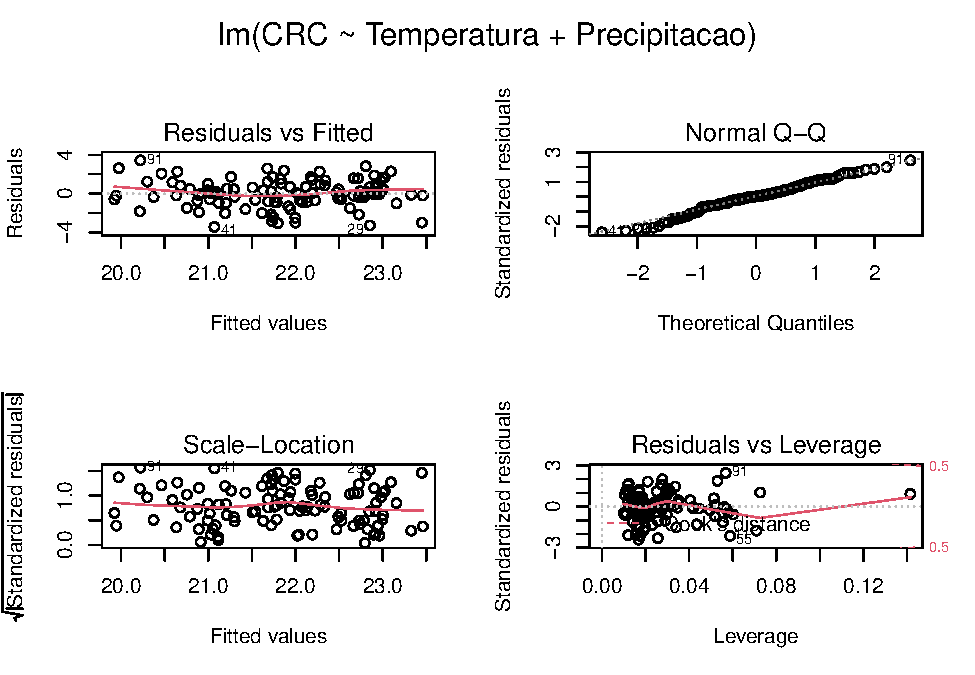
\includegraphics{livro_r_ecologia_files/figure-latex/unnamed-chunk-11-1.pdf}

\begin{Shaded}
\begin{Highlighting}[]
\KeywordTok{dev.off}\NormalTok{()}
\end{Highlighting}
\end{Shaded}

\begin{verbatim}
## null device 
##           1
\end{verbatim}

\begin{Shaded}
\begin{Highlighting}[]
\CommentTok{# VERIFICANDO OS RESULTADOS DA REGRESSÃO}
\CommentTok{#****************************************}
\KeywordTok{anova}\NormalTok{(modelo_regressao_mul)}
\end{Highlighting}
\end{Shaded}

\begin{verbatim}
## Analysis of Variance Table
## 
## Response: CRC
##               Df  Sum Sq Mean Sq F value   Pr(>F)    
## Temperatura    1  80.931  80.931 39.0028 8.94e-09 ***
## Precipitacao   1   2.549   2.549  1.2283   0.2702    
## Residuals    106 219.951   2.075                     
## ---
## Signif. codes:  0 '***' 0.001 '**' 0.01 '*' 0.05 '.' 0.1 ' ' 1
\end{verbatim}

\begin{Shaded}
\begin{Highlighting}[]
\CommentTok{# ou}
\KeywordTok{summary}\NormalTok{(modelo_regressao_mul)}
\end{Highlighting}
\end{Shaded}

\begin{verbatim}
## 
## Call:
## lm(formula = CRC ~ Temperatura + Precipitacao, data = dados_regressao_mul)
## 
## Residuals:
##     Min      1Q  Median      3Q     Max 
## -3.4351 -0.8026  0.0140  0.9420  3.4300 
## 
## Coefficients:
##                Estimate Std. Error t value Pr(>|t|)    
## (Intercept)  16.7162571  1.0108674  16.537  < 2e-16 ***
## Temperatura   0.2787445  0.0439601   6.341 5.71e-09 ***
## Precipitacao -0.0004270  0.0003852  -1.108     0.27    
## ---
## Signif. codes:  0 '***' 0.001 '**' 0.01 '*' 0.05 '.' 0.1 ' ' 1
## 
## Residual standard error: 1.44 on 106 degrees of freedom
## Multiple R-squared:  0.2751,	Adjusted R-squared:  0.2614 
## F-statistic: 20.12 on 2 and 106 DF,  p-value: 3.927e-08
\end{verbatim}

Percebam que a temperatura tem uma relação significativa com o tamanho do CRC das populações (P \textless{} 0.001), enquanto que a precipitação não apresenta relação com o CRC (P = 0.27). Neste caso, é interessante saber se um modelo mais simples (e.g.~contendo apenas temperatura) explicaria a distribuição tão bem ou melhor do que este modelo mais complexo considerando dois parâmetros (temperatura e precipitação).

Para isso, podemos utilizar a \emph{LIKELIHOOD RATIO TEST (LRT)} para comparar modelos. A LRT compara dois modelos aninhados, testando se os parâmetros do modelo mais complexo diferem significativamente do modelo mais simples.Em outras palavras, ele testa se há necessidade de se incluir um parâmetro extra no modelo para explicar os dados.

\begin{Shaded}
\begin{Highlighting}[]
\CommentTok{## CRIANDO OS MODELOS ANINHADOS}
\CommentTok{#********************************}
\NormalTok{modelo_regressao_mul <-}\StringTok{ }\KeywordTok{lm}\NormalTok{(CRC }\OperatorTok{~}\StringTok{ }\NormalTok{Temperatura }\OperatorTok{+}\StringTok{ }\NormalTok{Precipitacao, }\DataTypeTok{data =}\NormalTok{ dados_regressao_mul)}
\NormalTok{modelo_regressao <-}\StringTok{ }\KeywordTok{lm}\NormalTok{(CRC }\OperatorTok{~}\StringTok{ }\NormalTok{Temperatura, }\DataTypeTok{data =}\NormalTok{ dados_regressao_mul)}

\CommentTok{# LIKELIHHOD RATIO }\AlertTok{TEST}\CommentTok{ (LRT)}
\CommentTok{#*******************************}
\CommentTok{# A hipótese nula é que o modelo mais simples é melhor}
\CommentTok{# Valores de p < 0.05 rejeita a hipótese nula e o modelo mais complexo é o melhor}
\CommentTok{# Valores de p > 0.05 não rejeita a hipótese nula e o modelo mais simples é o melhor}
\KeywordTok{library}\NormalTok{(lmtest)}
\KeywordTok{lrtest}\NormalTok{(modelo_regressao_mul, modelo_regressao)}
\end{Highlighting}
\end{Shaded}

\begin{verbatim}
## Likelihood ratio test
## 
## Model 1: CRC ~ Temperatura + Precipitacao
## Model 2: CRC ~ Temperatura
##   #Df  LogLik Df  Chisq Pr(>Chisq)
## 1   4 -192.93                     
## 2   3 -193.55 -1 1.2558     0.2624
\end{verbatim}

\begin{Shaded}
\begin{Highlighting}[]
\CommentTok{# COMPARANDO COM O MODELO SOMENTE COM O INTERCEPTO}
\CommentTok{#************************************************}
\CommentTok{# criando um modelo sem parâmetros, só o intercepto}
\NormalTok{modelo_intercepto <-}\StringTok{ }\KeywordTok{lm}\NormalTok{(CRC }\OperatorTok{~}\StringTok{ }\DecValTok{1}\NormalTok{, }\DataTypeTok{data =}\NormalTok{ dados_regressao_mul)}
\KeywordTok{lrtest}\NormalTok{(modelo_regressao, modelo_intercepto)}
\end{Highlighting}
\end{Shaded}

\begin{verbatim}
## Likelihood ratio test
## 
## Model 1: CRC ~ Temperatura
## Model 2: CRC ~ 1
##   #Df  LogLik Df  Chisq Pr(>Chisq)    
## 1   3 -193.55                         
## 2   2 -210.46 -1 33.815  6.061e-09 ***
## ---
## Signif. codes:  0 '***' 0.001 '**' 0.01 '*' 0.05 '.' 0.1 ' ' 1
\end{verbatim}

\textbf{Interpretação dos resultados}

Neste exemplo, a precipitação não está associada com a variação no tamanho do CRC das populações de \emph{D. minutus}. Por outro lado, temperatura explicou 26\% da variação do tamanho do CRC das populações.

~

\hypertarget{anuxe1lises-de-variuxe2ncia-anova}{%
\section{Análises de Variância (ANOVA)}\label{anuxe1lises-de-variuxe2ncia-anova}}

\hypertarget{backgorund-da-anuxe1lise-5}{%
\subsection{Backgorund da análise}\label{backgorund-da-anuxe1lise-5}}

Anova refere-se a uma variedade de delineamentos experimentais nos quais a variável preditora é categórica e a variável resposta é contínua (Gotelli \& Ellison 2013). Exemplos desses delineamentos experimentais são: Anova de um fator, Anova de dois fatores, Anova em blocos aleatorizados, Anova de medidas repetidas e Anova \emph{split-splot}. De forma geral, a Anova é um teste estatístico usado para comparar a média entre grupos amostrados independentementes. Para isso, o teste leva em conta, além das médias dos grupos, a variação dos dados dentro e entre os grupos. Neste capítulo, iremos demonstrar as linhas de comandos para alguns dos principais delineamentos experimentais.

\begin{quote}
\hypertarget{premissas-da-anova}{%
\subsubsection{Premissas da Anova:}\label{premissas-da-anova}}

\begin{itemize}
\tightlist
\item
  As amostras devem ser independentes;
\item
  As unidades amostrais são selecionadas aleatoriamente;
\item
  Distribuição normal (gaussiana) dos resíduos;
\item
  Homogeneidade da variância.
\end{itemize}
\end{quote}

~

\hypertarget{anova-de-um-fator}{%
\section{ANOVA de um fator}\label{anova-de-um-fator}}

Este teste considera delineamentos experimentais com apenas um fator (ou tratamento) que pode ser composto por três ou mais grupos (ou níveis).

\hypertarget{exemplo-pruxe1tico-1---anova-de-um-fator}{%
\subsubsection{Exemplo prático 1 - Anova de um fator}\label{exemplo-pruxe1tico-1---anova-de-um-fator}}

\hypertarget{explicauxe7uxe3o-dos-dados-6}{%
\paragraph{Explicação dos dados}\label{explicauxe7uxe3o-dos-dados-6}}

Neste exemplo, avaliaremos se o adubo X-2020 disponibilizado recentemente no mercado melhora o crescimento dos indivíduos de \emph{Coffea arabica} como divulgado pela empresa responsável pela venda do produto. Para isso, foi realizado um experimento com indivíduos de \emph{C. arabica} cultivados em três grupos: i) grupo controle onde os indivíduos não receberam adubação, ii) grupo onde os indivíduos receberam a adição do adubo tradicional mais utilizado pelos produtores de \emph{C. arabica}, e iii) grupo onde os indivíduos receberam a adição do adubo X-2020.

\textbf{Pergunta:}

\begin{quote}
O crescimento dos indivíduos de \emph{C. arabica} é melhorado pela adição do adubo X-2020?
\end{quote}

\textbf{Predições}

\begin{quote}
O crescimento dos indivíduos de \emph{C. arabica} será maior no grupo que recebeu o adubo X-2020.
\end{quote}

\textbf{Variáveis}

\begin{itemize}
\tightlist
\item
  Variáveis preditoras

  \begin{itemize}
  \tightlist
  \item
    Dataframe com as plantas (unidade amostral) nas linhas e o tratamento na coluna.
  \end{itemize}
\end{itemize}

\textbf{Checklist}

\begin{itemize}
\tightlist
\item
  Verificar se o seu dataframe está com as unidades amostrais nas linhas e variável preditora na coluna.
\end{itemize}

\hypertarget{anuxe1lise-6}{%
\subsection{Análise}\label{anuxe1lise-6}}

Cálculo da Anova de um fator

\begin{Shaded}
\begin{Highlighting}[]
\CommentTok{## IMPORTANDO DADOS}
\CommentTok{#********************}
\NormalTok{dados_anova_simples <-}\StringTok{ }\NormalTok{ecodados}\OperatorTok{::}\NormalTok{anova_simples}
\KeywordTok{head}\NormalTok{(dados_anova_simples) }\CommentTok{# verificar se o dataframe foi lido corretamente}
\end{Highlighting}
\end{Shaded}

\begin{verbatim}
##   Crescimento Tratamento
## 1       7.190   Controle
## 2       6.758   Controle
## 3       6.101   Controle
## 4       4.758   Controle
## 5       6.542   Controle
## 6       7.667   Controle
\end{verbatim}

\begin{Shaded}
\begin{Highlighting}[]
\CommentTok{# ANALISE ANOVA de um fator}
\CommentTok{#************************}
\NormalTok{Modelo_anova <-}\StringTok{ }\KeywordTok{aov}\NormalTok{(Crescimento }\OperatorTok{~}\StringTok{ }\NormalTok{Tratamento, }\DataTypeTok{data =}\NormalTok{ dados_anova_simples) }

\CommentTok{# VERIFICANDO A NORMALIDADE E HOMOGENEIDADE DAS VARIÂNCIAS}
\CommentTok{#***********************************************************************}
\CommentTok{# Os gráficos *Residuals vs Fitted* e *Scale-Location* estão relacionados com a homogeneidade da variância. Nestes gráficos, esperamos ver os pontos dispersos no espaço sem padrões em forma de *U* ou funil. }
\CommentTok{# O gráfico *Normal Q-Q* está relacionado com a distribuição normal dos resíduos. Neste gráfico, esperamos ver os pontos próximos a reta sem padrões em forma de *U* ou *S*. }
\KeywordTok{par}\NormalTok{(}\DataTypeTok{mfrow =} \KeywordTok{c}\NormalTok{(}\DecValTok{2}\NormalTok{, }\DecValTok{2}\NormalTok{), }\DataTypeTok{oma =} \KeywordTok{c}\NormalTok{(}\DecValTok{0}\NormalTok{, }\DecValTok{0}\NormalTok{, }\DecValTok{2}\NormalTok{, }\DecValTok{0}\NormalTok{))}
\KeywordTok{plot}\NormalTok{(Modelo_anova)}
\end{Highlighting}
\end{Shaded}

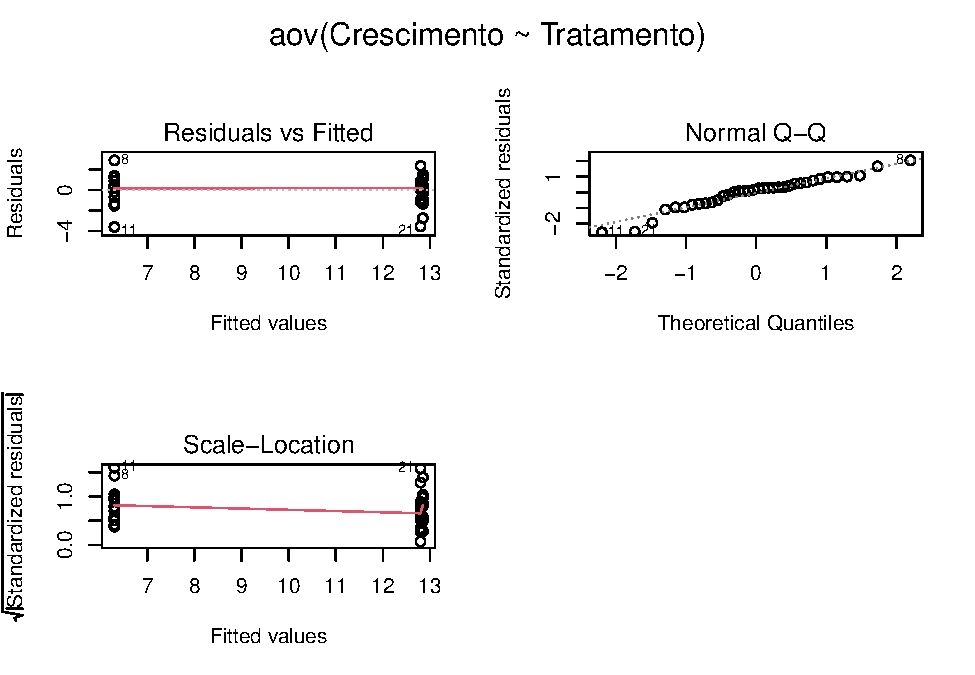
\includegraphics{livro_r_ecologia_files/figure-latex/unnamed-chunk-13-1.pdf}

\begin{Shaded}
\begin{Highlighting}[]
\KeywordTok{dev.off}\NormalTok{()}
\end{Highlighting}
\end{Shaded}

\begin{verbatim}
## null device 
##           1
\end{verbatim}

\begin{Shaded}
\begin{Highlighting}[]
\CommentTok{# Se preferir, você pode utilizar testes estatísticos}
\CommentTok{# Teste de Shapiro-Wilk para normalidade separadamente para cada grupo}
\KeywordTok{shapiro.test}\NormalTok{(dados_anova_simples}\OperatorTok{$}\NormalTok{Crescimento[}\DecValTok{1}\OperatorTok{:}\DecValTok{12}\NormalTok{])}
\end{Highlighting}
\end{Shaded}

\begin{verbatim}
## 
## 	Shapiro-Wilk normality test
## 
## data:  dados_anova_simples$Crescimento[1:12]
## W = 0.96731, p-value = 0.8806
\end{verbatim}

\begin{Shaded}
\begin{Highlighting}[]
\KeywordTok{shapiro.test}\NormalTok{(dados_anova_simples}\OperatorTok{$}\NormalTok{Crescimento[}\DecValTok{13}\OperatorTok{:}\DecValTok{24}\NormalTok{])}
\end{Highlighting}
\end{Shaded}

\begin{verbatim}
## 
## 	Shapiro-Wilk normality test
## 
## data:  dados_anova_simples$Crescimento[13:24]
## W = 0.87324, p-value = 0.07184
\end{verbatim}

\begin{Shaded}
\begin{Highlighting}[]
\KeywordTok{shapiro.test}\NormalTok{(dados_anova_simples}\OperatorTok{$}\NormalTok{Crescimento[}\DecValTok{25}\OperatorTok{:}\DecValTok{36}\NormalTok{])}
\end{Highlighting}
\end{Shaded}

\begin{verbatim}
## 
## 	Shapiro-Wilk normality test
## 
## data:  dados_anova_simples$Crescimento[25:36]
## W = 0.9294, p-value = 0.3738
\end{verbatim}

\begin{Shaded}
\begin{Highlighting}[]
\CommentTok{# Teste de Bartlett para homogeneidade da variância}
\KeywordTok{bartlett.test}\NormalTok{(Crescimento }\OperatorTok{~}\StringTok{ }\NormalTok{Tratamento, }\DataTypeTok{data =}\NormalTok{ dados_anova_simples)}
\end{Highlighting}
\end{Shaded}

\begin{verbatim}
## 
## 	Bartlett test of homogeneity of variances
## 
## data:  Crescimento by Tratamento
## Bartlett's K-squared = 0.61835, df = 2, p-value = 0.7341
\end{verbatim}

\begin{Shaded}
\begin{Highlighting}[]
\CommentTok{# VERIFICANDO OS RESULTADOS DA ANOVA}
\CommentTok{#****************************************}
\KeywordTok{anova}\NormalTok{(Modelo_anova)}
\end{Highlighting}
\end{Shaded}

\begin{verbatim}
## Analysis of Variance Table
## 
## Response: Crescimento
##            Df Sum Sq Mean Sq F value    Pr(>F)    
## Tratamento  2 340.32 170.160  77.989 3.124e-13 ***
## Residuals  33  72.00   2.182                      
## ---
## Signif. codes:  0 '***' 0.001 '**' 0.01 '*' 0.05 '.' 0.1 ' ' 1
\end{verbatim}

Percebam que o resultado da Anova (Pr(\textgreater F) \textless{} 0.001) indica que devemos rejeitar a hipótese nula que não há diferença entre as médias dos grupos. Contudo, os resultados não mostram quais são os grupos que apresentam diferenças. Para isso, temos que realizar testes de comparações múltiplas \emph{post-hoc} para detectar os grupos que apresentam diferenças significativas entre as médias. \textbf{Observação} Os testes \emph{post-hoc} só devem ser utilizados quando rejeitamos a hipótese nula (P \textless{} 0.05) no teste da Anova.

\begin{Shaded}
\begin{Highlighting}[]
\CommentTok{# Diferenças entre os tratamentos}
\CommentTok{#***********************************}
\CommentTok{# Teste de Tuckey's honest significant difference}
\KeywordTok{TukeyHSD}\NormalTok{(Modelo_anova)}
\end{Highlighting}
\end{Shaded}

\begin{verbatim}
##   Tukey multiple comparisons of means
##     95% family-wise confidence level
## 
## Fit: aov(formula = Crescimento ~ Tratamento, data = dados_anova_simples)
## 
## $Tratamento
##                                       diff       lwr       upr     p adj
## Adubo_X-2020-Adubo_Tradicional  0.04991667 -1.429784  1.529617 0.9962299
## Controle-Adubo_Tradicional     -6.49716667 -7.976867 -5.017466 0.0000000
## Controle-Adubo_X-2020          -6.54708333 -8.026784 -5.067383 0.0000000
\end{verbatim}

\begin{Shaded}
\begin{Highlighting}[]
\CommentTok{# ou}

\CommentTok{# Teste T}
\KeywordTok{pairwise.t.test}\NormalTok{(dados_anova_simples}\OperatorTok{$}\NormalTok{Crescimento, dados_anova_simples}\OperatorTok{$}\NormalTok{Tratamento)}
\end{Highlighting}
\end{Shaded}

\begin{verbatim}
## 
## 	Pairwise comparisons using t tests with pooled SD 
## 
## data:  dados_anova_simples$Crescimento and dados_anova_simples$Tratamento 
## 
##              Adubo_Tradicional Adubo_X-2020
## Adubo_X-2020 0.93              -           
## Controle     6e-12             6e-12       
## 
## P value adjustment method: holm
\end{verbatim}

Visualizar os resultados em gráfico

\begin{Shaded}
\begin{Highlighting}[]
\CommentTok{# Reordenando a ordem que os grupos irão aparecer no gráfico}
\NormalTok{dados_anova_simples}\OperatorTok{$}\NormalTok{Tratamento <-}\StringTok{ }\KeywordTok{factor}\NormalTok{(dados_anova_simples}\OperatorTok{$}\NormalTok{Tratamento , }
                                      \DataTypeTok{levels=}\KeywordTok{c}\NormalTok{(}\StringTok{"Controle"}\NormalTok{, }\StringTok{"Adubo_Tradicional"}\NormalTok{, }\StringTok{"Adubo_X-2020"}\NormalTok{))}

\CommentTok{# Gráfico}
\KeywordTok{library}\NormalTok{(ggplot2)}
\KeywordTok{ggplot}\NormalTok{(}\DataTypeTok{data =}\NormalTok{ dados_anova_simples, }\KeywordTok{aes}\NormalTok{(}\DataTypeTok{x=}\NormalTok{ Tratamento, }\DataTypeTok{y=}\NormalTok{ Crescimento, }\DataTypeTok{color =}\NormalTok{ Tratamento)) }\OperatorTok{+}\StringTok{ }
\StringTok{  }\KeywordTok{labs}\NormalTok{(}\DataTypeTok{x =} \StringTok{"Adubação"}\NormalTok{, }\DataTypeTok{y =} \StringTok{"Crescimento Coffea arabica (cm)"}\NormalTok{, }\DataTypeTok{size =} \DecValTok{20}\NormalTok{) }\OperatorTok{+}
\StringTok{  }\KeywordTok{geom_boxplot}\NormalTok{(}\DataTypeTok{fill=}\KeywordTok{c}\NormalTok{(}\StringTok{"steelblue1"}\NormalTok{, }\StringTok{"springgreen1"}\NormalTok{, }\StringTok{"brown1"}\NormalTok{), }\DataTypeTok{color=}\StringTok{"black"}\NormalTok{, }\DataTypeTok{show.legend =} \OtherTok{FALSE}\NormalTok{,}
               \DataTypeTok{alpha =} \FloatTok{0.4}\NormalTok{) }\OperatorTok{+}
\StringTok{  }\KeywordTok{geom_jitter}\NormalTok{(}\DataTypeTok{shape =} \DecValTok{16}\NormalTok{, }\DataTypeTok{position=}\KeywordTok{position_jitter}\NormalTok{(}\FloatTok{0.1}\NormalTok{), }\DataTypeTok{cex =} \DecValTok{4}\NormalTok{, }\DataTypeTok{alpha =} \FloatTok{0.7}\NormalTok{) }\OperatorTok{+}
\StringTok{  }\KeywordTok{scale_color_manual}\NormalTok{(}\DataTypeTok{values =} \KeywordTok{c}\NormalTok{(}\StringTok{"steelblue1"}\NormalTok{, }\StringTok{"springgreen1"}\NormalTok{, }\StringTok{"brown1"}\NormalTok{)) }\OperatorTok{+}
\StringTok{  }\KeywordTok{scale_y_continuous}\NormalTok{(}\DataTypeTok{limits =} \KeywordTok{c}\NormalTok{(}\DecValTok{0}\NormalTok{, }\DecValTok{20}\NormalTok{), }\DataTypeTok{breaks =} \KeywordTok{c}\NormalTok{(}\DecValTok{0}\NormalTok{, }\DecValTok{5}\NormalTok{, }\DecValTok{10}\NormalTok{, }\DecValTok{15}\NormalTok{, }\DecValTok{20}\NormalTok{)) }\OperatorTok{+}
\StringTok{  }\KeywordTok{geom_text}\NormalTok{(}\DataTypeTok{x =} \DecValTok{1}\NormalTok{, }\DataTypeTok{y =} \DecValTok{12}\NormalTok{, }\DataTypeTok{label =} \StringTok{"ab"}\NormalTok{, }\DataTypeTok{color =} \StringTok{"black"}\NormalTok{, }\DataTypeTok{size =} \DecValTok{5}\NormalTok{) }\OperatorTok{+}
\StringTok{  }\KeywordTok{geom_text}\NormalTok{(}\DataTypeTok{x =} \DecValTok{2}\NormalTok{, }\DataTypeTok{y =} \DecValTok{17}\NormalTok{, }\DataTypeTok{label =} \StringTok{"a"}\NormalTok{, }\DataTypeTok{color =} \StringTok{"black"}\NormalTok{, }\DataTypeTok{size =} \DecValTok{5}\NormalTok{) }\OperatorTok{+}
\StringTok{  }\KeywordTok{geom_text}\NormalTok{(}\DataTypeTok{x =} \DecValTok{3}\NormalTok{, }\DataTypeTok{y =} \DecValTok{17}\NormalTok{, }\DataTypeTok{label =} \StringTok{"b"}\NormalTok{, }\DataTypeTok{color =} \StringTok{"black"}\NormalTok{, }\DataTypeTok{size =} \DecValTok{5}\NormalTok{) }\OperatorTok{+}
\StringTok{  }\KeywordTok{scale_x_discrete}\NormalTok{(}\DataTypeTok{labels=}\KeywordTok{c}\NormalTok{(}\StringTok{"Sem adubo"}\NormalTok{,}\StringTok{"Tradicional"}\NormalTok{,}\StringTok{"X-2020"}\NormalTok{)) }\OperatorTok{+}
\StringTok{  }\KeywordTok{theme_bw}\NormalTok{() }\OperatorTok{+}
\StringTok{  }\KeywordTok{theme}\NormalTok{(}\DataTypeTok{axis.title.y =} \KeywordTok{element_text}\NormalTok{(}\DataTypeTok{size =} \DecValTok{17}\NormalTok{), }\DataTypeTok{axis.title.x =} \KeywordTok{element_text}\NormalTok{(}\DataTypeTok{size =} \DecValTok{17}\NormalTok{)) }\OperatorTok{+}
\StringTok{  }\KeywordTok{theme}\NormalTok{(}\DataTypeTok{axis.text.y =} \KeywordTok{element_text}\NormalTok{(}\DataTypeTok{size =} \DecValTok{17}\NormalTok{), }\DataTypeTok{axis.text.x =} \KeywordTok{element_text}\NormalTok{(}\DataTypeTok{size =} \DecValTok{17}\NormalTok{)) }\OperatorTok{+}
\StringTok{  }\KeywordTok{theme}\NormalTok{(}\DataTypeTok{panel.grid.major =} \KeywordTok{element_blank}\NormalTok{(), }\DataTypeTok{panel.grid.minor =} \KeywordTok{element_blank}\NormalTok{(), }
        \DataTypeTok{panel.border =} \KeywordTok{element_rect}\NormalTok{(}\DataTypeTok{colour =} \StringTok{"black"}\NormalTok{, }\DataTypeTok{fill=}\OtherTok{NA}\NormalTok{, }\DataTypeTok{size =} \DecValTok{2}\NormalTok{)) }\OperatorTok{+}
\StringTok{  }\KeywordTok{theme}\NormalTok{(}\DataTypeTok{legend.position =} \StringTok{"none"}\NormalTok{) }
\end{Highlighting}
\end{Shaded}

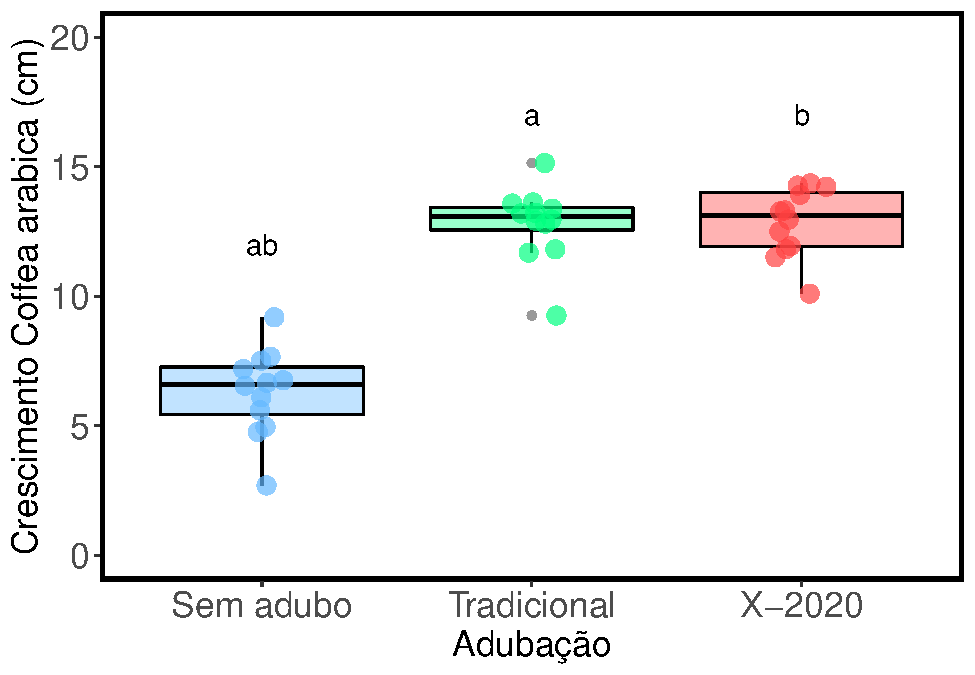
\includegraphics{livro_r_ecologia_files/figure-latex/unnamed-chunk-15-1.pdf}

\textbf{Interpretação dos resultados}

Neste exemplo, os indivíduos de \emph{C. arabica} que receberam adubação (tradicional e X-2020) apresentaram maior crescimento do que os indivíduos que não receberam adubação. Contudo, diferente do que foi divulgado pela empresa, o adubo X-2020 não apresentou melhor desempenho que o adubo tradicional já utilizado pelos produtores.

~

\hypertarget{anova-de-dois-fatores-ou-anova-fatorial}{%
\section{ANOVA de dois fatores ou Anova fatorial}\label{anova-de-dois-fatores-ou-anova-fatorial}}

Este teste considera delineamentos amostrais com dois fatores (ou tratamento) que podem ser compostos por dois ou mais grupos (ou níveis). Esta análise tem uma vantagem, pois permite avaliar o efeito da interação entre os fatores na variável resposta. Quando a interação está presente, o impacto de um fator depende do nível (ou grupo) do outro fator.

\hypertarget{exemplo-pruxe1tico-1---anova-de-dois-fatores}{%
\subsubsection{Exemplo prático 1 - Anova de dois fatores}\label{exemplo-pruxe1tico-1---anova-de-dois-fatores}}

\hypertarget{explicauxe7uxe3o-dos-dados-7}{%
\paragraph{Explicação dos dados}\label{explicauxe7uxe3o-dos-dados-7}}

Neste exemplo, avaliaremos se o tempo que o corpo leva para elimiar uma droga utilizada em exames de ressonância magnética está relacionado com o sistema XY de determinação do sexo e/ou com a idade dos pacientes. Para isso, foi realizado um experimento com 40 pacientes distribuídos da seguinte maneira: i) 10 indivíduos XX - jovens, ii) 10 indivíduos XX - idosas, iii) 10 indivíduos XY - jovens, e iv) 10 indivíduos XY - idosos.

\textbf{Pergunta:}

\begin{quote}
O tempo de eliminação da droga é dependente do sistema XY de determinação do sexo e idade dos pacientes?
\end{quote}

\textbf{Predições}

\begin{quote}
O tempo de eliminação da droga vai ser mais rápido nas pacientes XX e jovens.
\end{quote}

\textbf{Variáveis}

\begin{itemize}
\tightlist
\item
  Variáveis preditoras

  \begin{itemize}
  \tightlist
  \item
    Dataframe com os pacientes (unidade amostral) nas linhas e os tratamentos nas colunas.
  \end{itemize}
\end{itemize}

\textbf{Checklist}

\begin{itemize}
\tightlist
\item
  Verificar se o seu dataframe está com as unidades amostrais nas linhas e as variáveies preditoras nas colunas.
\end{itemize}

\hypertarget{anuxe1lise-7}{%
\subsection{Análise}\label{anuxe1lise-7}}

Cálculo da Anova de dois fator

\begin{Shaded}
\begin{Highlighting}[]
\CommentTok{## IMPORTANDO DADOS}
\CommentTok{#********************}
\NormalTok{dados_dois_fatores <-}\StringTok{ }\NormalTok{ecodados}\OperatorTok{::}\NormalTok{anova_dois_fatores}
\KeywordTok{head}\NormalTok{(dados_dois_fatores) }
\end{Highlighting}
\end{Shaded}

\begin{verbatim}
##    Tempo Pessoas Idade
## 1 18.952      XX Jovem
## 2 16.513      XX Jovem
## 3 17.981      XX Jovem
## 4 21.371      XX Jovem
## 5 14.470      XX Jovem
## 6 19.130      XX Jovem
\end{verbatim}

\begin{Shaded}
\begin{Highlighting}[]
\CommentTok{# Análise anova de dois fatores }
\CommentTok{#********************************}
\CommentTok{# A interação entre os fatores é representada por *}
\NormalTok{Modelo1 <-}\StringTok{ }\KeywordTok{aov}\NormalTok{(Tempo }\OperatorTok{~}\StringTok{ }\NormalTok{Pessoas }\OperatorTok{*}\StringTok{ }\NormalTok{Idade, }\DataTypeTok{data =}\NormalTok{ dados_dois_fatores) }

\CommentTok{# Olhando os resultados}
\KeywordTok{anova}\NormalTok{(Modelo1)}
\end{Highlighting}
\end{Shaded}

\begin{verbatim}
## Analysis of Variance Table
## 
## Response: Tempo
##               Df  Sum Sq Mean Sq  F value    Pr(>F)    
## Pessoas        1  716.72  716.72 178.8538  1.56e-15 ***
## Idade          1 1663.73 1663.73 415.1724 < 2.2e-16 ***
## Pessoas:Idade  1    4.77    4.77   1.1903    0.2825    
## Residuals     36  144.26    4.01                       
## ---
## Signif. codes:  0 '***' 0.001 '**' 0.01 '*' 0.05 '.' 0.1 ' ' 1
\end{verbatim}

\begin{Shaded}
\begin{Highlighting}[]
\CommentTok{# Percebam que a interação não apresenta um efeito significativo (P > 0.05). Assim, iremos retirar a interação e verificar, usando LIKELIHOOD RATIO }\AlertTok{TEST}\CommentTok{ (LRT), se o modelo mais simples é melhor }
\NormalTok{Modelo2 <-}\StringTok{ }\KeywordTok{aov}\NormalTok{(Tempo }\OperatorTok{~}\StringTok{ }\NormalTok{Pessoas }\OperatorTok{+}\StringTok{ }\NormalTok{Idade, }\DataTypeTok{data =}\NormalTok{ dados_dois_fatores) }

\CommentTok{# A hipótese nula é que o modelo mais simples é melhor}
\CommentTok{# Valores de p < 0.05 rejeita a hipótese nula e o modelo mais complexo é o melhor}
\CommentTok{# Valores de p > 0.05 não rejeita a hipótese nula e o modelo mais simples é o melhor}
\KeywordTok{library}\NormalTok{(lmtest)}
\KeywordTok{lrtest}\NormalTok{(Modelo1, Modelo2)}
\end{Highlighting}
\end{Shaded}

\begin{verbatim}
## Likelihood ratio test
## 
## Model 1: Tempo ~ Pessoas * Idade
## Model 2: Tempo ~ Pessoas + Idade
##   #Df  LogLik Df  Chisq Pr(>Chisq)
## 1   5 -82.413                     
## 2   4 -83.063 -1 1.3012      0.254
\end{verbatim}

\begin{Shaded}
\begin{Highlighting}[]
\CommentTok{# VERIFICANDO A NORMALIDADE E HOMOGENEIDADE DAS VARIÂNCIAS}
\CommentTok{#***********************************************************************}
\CommentTok{# Esta função mostra os resultados para multicolinearidade (a), dois gráficos avaliando a normalidade dos resíduos (b e  c), e um gráfico para a homogeneidade dos resíduos (d).}
\KeywordTok{library}\NormalTok{(sjPlot)}
\KeywordTok{plot_grid}\NormalTok{(}\KeywordTok{plot_model}\NormalTok{(Modelo2, }\DataTypeTok{type =} \StringTok{"diag"}\NormalTok{))}
\end{Highlighting}
\end{Shaded}

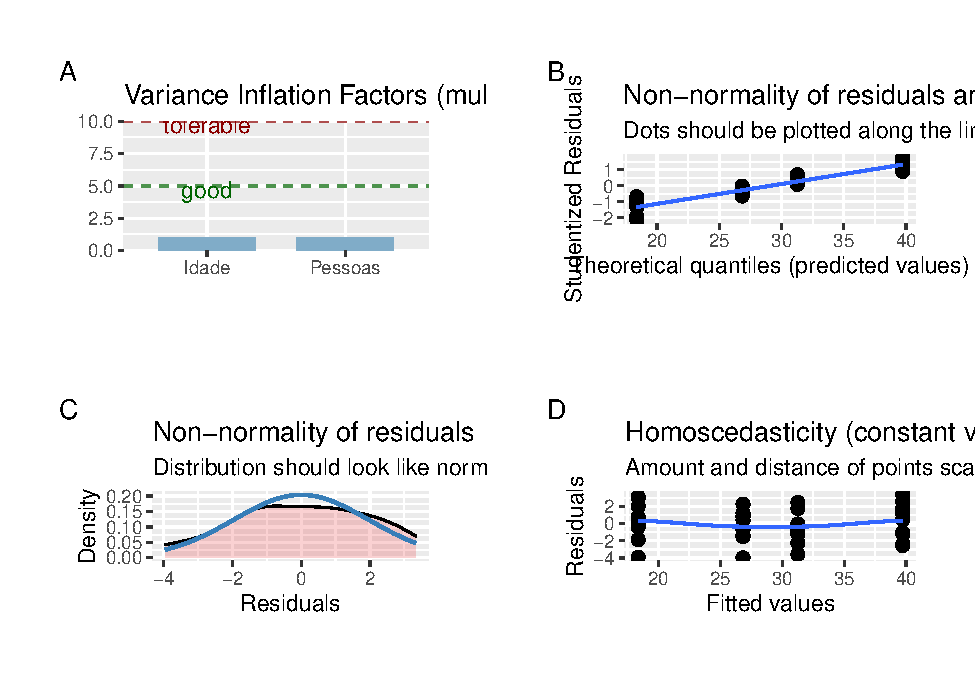
\includegraphics{livro_r_ecologia_files/figure-latex/unnamed-chunk-16-1.pdf}

\begin{Shaded}
\begin{Highlighting}[]
\CommentTok{# VERIFICANDO OS RESULTADOS DA ANOVA}
\CommentTok{#****************************************}
\KeywordTok{anova}\NormalTok{(Modelo2)}
\end{Highlighting}
\end{Shaded}

\begin{verbatim}
## Analysis of Variance Table
## 
## Response: Tempo
##           Df  Sum Sq Mean Sq F value    Pr(>F)    
## Pessoas    1  716.72  716.72  177.94 1.041e-15 ***
## Idade      1 1663.73 1663.73  413.05 < 2.2e-16 ***
## Residuals 37  149.03    4.03                      
## ---
## Signif. codes:  0 '***' 0.001 '**' 0.01 '*' 0.05 '.' 0.1 ' ' 1
\end{verbatim}

Percebam que o resultado da Anova (Pr(\textgreater F) \textless{} 0.001) indica que devemos rejeitar a hipótese nula que não há diferença entre as médias dos sistema XY e idade dos pacientes. Neste caso, não precisamos realizar testes de comparações múltiplas \emph{post-hoc} porque os fatores apresentam apenas dois níveis. Contudo, se no seu delineamento experimental um dos fatores apresentar três ou mais níveis, você deverá utilizar os testes de comparações \emph{post-hoc} para determinar as diferenças entre os grupos. \textbf{Observação} Os testes \emph{post-hoc} só devem ser utilizados quando rejeitamos a hipótese nula (P \textless{} 0.05) no teste da Anova.

\begin{Shaded}
\begin{Highlighting}[]
\CommentTok{# Diferenças entre os tratamentos}
\CommentTok{#***********************************}
\CommentTok{# Teste de Tuckey's honest significant difference}
\KeywordTok{TukeyHSD}\NormalTok{(Modelo2)}
\end{Highlighting}
\end{Shaded}

\begin{verbatim}
##   Tukey multiple comparisons of means
##     95% family-wise confidence level
## 
## Fit: aov(formula = Tempo ~ Pessoas + Idade, data = dados_dois_fatores)
## 
## $Pessoas
##          diff      lwr      upr p adj
## XY-XX 8.46595 7.180008 9.751892     0
## 
## $Idade
##                  diff       lwr       upr p adj
## Jovem-Idoso -12.89855 -14.18449 -11.61261     0
\end{verbatim}

Visualizar os resultados em gráfico

\begin{Shaded}
\begin{Highlighting}[]
\CommentTok{# Gráfico}
\KeywordTok{library}\NormalTok{(ggplot2)}
\KeywordTok{ggplot}\NormalTok{(}\DataTypeTok{data =}\NormalTok{ dados_dois_fatores, }\KeywordTok{aes}\NormalTok{(}\DataTypeTok{y=}\NormalTok{ Tempo, }\DataTypeTok{x=}\NormalTok{ Pessoas, }\DataTypeTok{color =}\NormalTok{ Idade)) }\OperatorTok{+}\StringTok{ }
\StringTok{  }\KeywordTok{geom_boxplot}\NormalTok{() }\OperatorTok{+}
\StringTok{  }\KeywordTok{labs}\NormalTok{(}\DataTypeTok{x =} \StringTok{"Sistema XY de determinação do sexo"}\NormalTok{, }\DataTypeTok{y =} \StringTok{"Tempo (horas) para eliminar a droga"}\NormalTok{, }
       \DataTypeTok{size =} \DecValTok{20}\NormalTok{) }\OperatorTok{+}
\StringTok{  }\KeywordTok{geom_jitter}\NormalTok{(}\DataTypeTok{shape =} \DecValTok{16}\NormalTok{, }\DataTypeTok{position=}\KeywordTok{position_jitterdodge}\NormalTok{(), }\DataTypeTok{cex =} \DecValTok{4}\NormalTok{, }\DataTypeTok{alpha =} \FloatTok{0.7}\NormalTok{) }\OperatorTok{+}
\StringTok{  }\KeywordTok{scale_color_manual}\NormalTok{(}\DataTypeTok{values =} \KeywordTok{c}\NormalTok{(}\StringTok{"steelblue1"}\NormalTok{, }\StringTok{"springgreen1"}\NormalTok{)) }\OperatorTok{+}
\StringTok{  }\KeywordTok{scale_y_continuous}\NormalTok{(}\DataTypeTok{limits =} \KeywordTok{c}\NormalTok{(}\DecValTok{10}\NormalTok{, }\DecValTok{50}\NormalTok{), }\DataTypeTok{breaks =} \KeywordTok{c}\NormalTok{(}\DecValTok{10}\NormalTok{, }\DecValTok{20}\NormalTok{, }\DecValTok{30}\NormalTok{, }\DecValTok{40}\NormalTok{, }\DecValTok{50}\NormalTok{)) }\OperatorTok{+}
\StringTok{  }\KeywordTok{theme}\NormalTok{(}\DataTypeTok{axis.title.y =} \KeywordTok{element_text}\NormalTok{(}\DataTypeTok{size =} \DecValTok{17}\NormalTok{), }\DataTypeTok{axis.title.x =} \KeywordTok{element_text}\NormalTok{(}\DataTypeTok{size =} \DecValTok{17}\NormalTok{)) }\OperatorTok{+}
\StringTok{  }\KeywordTok{theme}\NormalTok{(}\DataTypeTok{axis.text.y =} \KeywordTok{element_text}\NormalTok{(}\DataTypeTok{size =} \DecValTok{17}\NormalTok{), }\DataTypeTok{axis.text.x =} \KeywordTok{element_text}\NormalTok{(}\DataTypeTok{size =} \DecValTok{17}\NormalTok{)) }\OperatorTok{+}
\StringTok{  }\KeywordTok{theme}\NormalTok{(}\DataTypeTok{panel.grid.minor =} \KeywordTok{element_blank}\NormalTok{(), }
        \DataTypeTok{panel.border =} \KeywordTok{element_rect}\NormalTok{(}\DataTypeTok{colour =} \StringTok{"black"}\NormalTok{, }\DataTypeTok{fill=}\OtherTok{NA}\NormalTok{, }\DataTypeTok{size =} \DecValTok{2}\NormalTok{)) }
\end{Highlighting}
\end{Shaded}

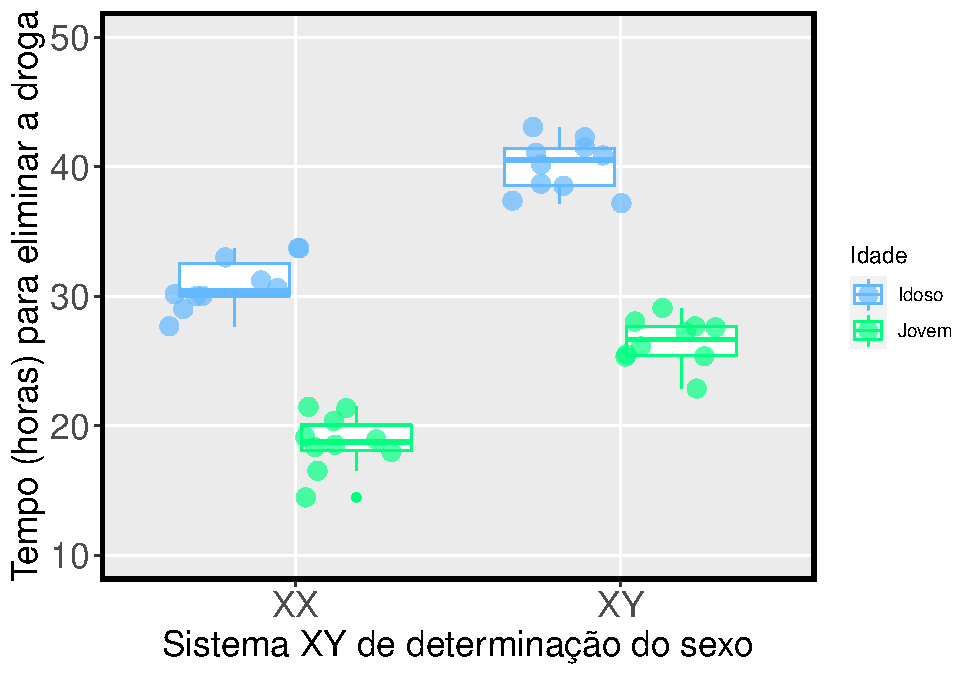
\includegraphics{livro_r_ecologia_files/figure-latex/unnamed-chunk-18-1.pdf}

\textbf{Interpretação dos resultados}

Neste exemplo, O sitesma XY de determinação do sexo e a idade dos pacientes tem um efeito no tempo de eliminação da droga do organismo. Os pacientes XX e jovens apresentam eliminação mais rápida da droga do que pacientes XY e idosos.

~

\hypertarget{anova-em-blocos-aleatorizados}{%
\section{ANOVA em blocos aleatorizados}\label{anova-em-blocos-aleatorizados}}

No delineamento experimental com blocos aleatorizados, cada fator é agrupado em blocos, com réplicas de cada nível do fator representado em cada bloco (Gotelli \& Elisson 2013). O bloco é uma área ou período de tempo dentro do qual as condições ambientais são relativamente homogêneas. O objetivo do uso dos blocos é controlar fontes de variações indesejadas na variável dependente que não são de interesse do pesquisador. Desta maneira, podemos retirar dos resíduos, os efeitos das variações indesejadas que não do nosso interesse, e testar com maior poder estatístico os efeitos dos tratamentos de interesse. Importante, os blocos devem ser arranjados de forma que as condições ambientais sejam mais similares dentro dos blocos do que entre os blocos.

~

\hypertarget{exemplo-pruxe1tico-1---anova-em-blocos-aleatorizados}{%
\subsubsection{Exemplo prático 1 - Anova em blocos aleatorizados}\label{exemplo-pruxe1tico-1---anova-em-blocos-aleatorizados}}

\hypertarget{explicauxe7uxe3o-dos-dados-8}{%
\paragraph{Explicação dos dados}\label{explicauxe7uxe3o-dos-dados-8}}

Neste exemplo, avaliaremos a riqueza de espécies de anuros amostradas em poças artificiais instaladas a diferentes distâncias de seis fragmentos florestais no sudeste do Brasil (da Silva et al.~2020). Os fragmentos florestais apresentam diferenças entre si que não do interesse do pesquisador. Por isso, eles foram incluídos como blocos nas análises. As poças artificiais foram instaladas em todos os fragmentos florestais basedo no seguinte delineamento experimental (da Silva et al.~2012): i) 4 poças no interior do fragmento a 100m de distância da borda do fragmento; ii) 4 poças no interior no fragmento a 50m de distância da borda do fragmento; iii) 4 poças no na borda do fragmento; iv) 4 poças na matriz de pastagem a 50m de distância da borda do fragmento; e v) 4 poças na matriz de pastagem a 100m de distância da borda do fragmento. Percebam que todos os tratamentos foram instalados em todos os blocos.

\textbf{Pergunta:}

\begin{quote}
A distância da poça artifical ao fragmento florestal influência a riqueza de espécies anuros?
\end{quote}

\textbf{Predições}

\begin{quote}
Poças na borda do fragmento florestal apresentarão maior riqueza de espécies do que poças distantes da borda.
\end{quote}

\textbf{Variáveis}

\begin{itemize}
\tightlist
\item
  Variáveis preditoras

  \begin{itemize}
  \tightlist
  \item
    Dataframe com as poças (unidade amostral) nas linhas e o tratamento e bloco nas colunas.
  \end{itemize}
\end{itemize}

\textbf{Checklist}

\begin{itemize}
\tightlist
\item
  Verificar se o seu dataframe está com as unidades amostrais nas linhas e variáveis preditoras nas colunas.
\end{itemize}

\hypertarget{anuxe1lise-8}{%
\subsection{Análise}\label{anuxe1lise-8}}

Cálculo da Anova em blocos aleatorizados

\begin{Shaded}
\begin{Highlighting}[]
\CommentTok{## IMPORTANDO DADOS}
\CommentTok{#********************}
\NormalTok{dados_bloco <-}\StringTok{ }\NormalTok{ecodados}\OperatorTok{::}\NormalTok{anova_bloco}
\KeywordTok{str}\NormalTok{(dados_bloco) }\CommentTok{# verificar se o dataframe foi lido corretamente}
\end{Highlighting}
\end{Shaded}

\begin{verbatim}
## 'data.frame':	30 obs. of  3 variables:
##  $ Riqueza: int  90 95 107 92 89 92 81 92 93 80 ...
##  $ Blocos : chr  "A" "A" "A" "A" ...
##  $ Pocas  : chr  "Int-50m" "Int-100m" "Borda" "Mat-50m" ...
\end{verbatim}

\begin{Shaded}
\begin{Highlighting}[]
\CommentTok{# ANALISE ANOVA em blocos aleatorizados}
\CommentTok{#****************************************}
\CommentTok{# Há duas maneiras para incluir os efeitos dos blocos}
\NormalTok{model_bloco1 <-}\StringTok{ }\KeywordTok{aov}\NormalTok{(Riqueza }\OperatorTok{~}\StringTok{ }\NormalTok{Pocas }\OperatorTok{+}\StringTok{ }\NormalTok{Blocos, }\DataTypeTok{data =}\NormalTok{ dados_bloco)}

\NormalTok{model_bloco2 <-}\StringTok{ }\KeywordTok{aov}\NormalTok{(Riqueza }\OperatorTok{~}\StringTok{ }\NormalTok{Pocas }\OperatorTok{+}\StringTok{ }\KeywordTok{Error}\NormalTok{(Blocos), }\DataTypeTok{data =}\NormalTok{ dados_bloco)}

\CommentTok{# Percebam que as duas formas apresentam os mesmo resultados para o efeito da distância das poças que é o fator de interesse no estudo. Lembre-se que nos delineamentos experimentais em bloco, o pesquisador não está interessado no efeito do bloco, mas sim controlar a variação associada a ele.}
\KeywordTok{anova}\NormalTok{(model_bloco1)}
\end{Highlighting}
\end{Shaded}

\begin{verbatim}
## Analysis of Variance Table
## 
## Response: Riqueza
##           Df Sum Sq Mean Sq F value Pr(>F)  
## Pocas      4 1504.5  376.12  2.9071 0.0478 *
## Blocos     5 1089.0  217.79  1.6834 0.1846  
## Residuals 20 2587.5  129.38                 
## ---
## Signif. codes:  0 '***' 0.001 '**' 0.01 '*' 0.05 '.' 0.1 ' ' 1
\end{verbatim}

\begin{Shaded}
\begin{Highlighting}[]
\KeywordTok{summary}\NormalTok{(model_bloco2)}
\end{Highlighting}
\end{Shaded}

\begin{verbatim}
## 
## Error: Blocos
##           Df Sum Sq Mean Sq F value Pr(>F)
## Residuals  5   1089   217.8               
## 
## Error: Within
##           Df Sum Sq Mean Sq F value Pr(>F)  
## Pocas      4   1504   376.1   2.907 0.0478 *
## Residuals 20   2588   129.4                 
## ---
## Signif. codes:  0 '***' 0.001 '**' 0.01 '*' 0.05 '.' 0.1 ' ' 1
\end{verbatim}

\begin{Shaded}
\begin{Highlighting}[]
\CommentTok{# O que não pode acontecer é ignorar o efeito do bloco que é incorporado pelos resíduos quando não informado no modelo. Veja abaixo a forma errada de analisar delineamento experimental com blocos.}

\NormalTok{modelo_errado <-}\StringTok{ }\KeywordTok{aov}\NormalTok{(Riqueza }\OperatorTok{~}\StringTok{ }\NormalTok{Pocas, }\DataTypeTok{data =}\NormalTok{ dados_bloco)}
\KeywordTok{anova}\NormalTok{(modelo_errado)}
\end{Highlighting}
\end{Shaded}

\begin{verbatim}
## Analysis of Variance Table
## 
## Response: Riqueza
##           Df Sum Sq Mean Sq F value  Pr(>F)  
## Pocas      4 1504.5  376.12  2.5576 0.06359 .
## Residuals 25 3676.5  147.06                  
## ---
## Signif. codes:  0 '***' 0.001 '**' 0.01 '*' 0.05 '.' 0.1 ' ' 1
\end{verbatim}

\begin{Shaded}
\begin{Highlighting}[]
\CommentTok{# VERIFICANDO A NORMALIDADE E HOMOGENEIDADE DAS VARIÂNCIAS}
\CommentTok{#***********************************************************************}
\CommentTok{# Os gráficos *Residuals vs Fitted* e *Scale-Location* estão relacionados com a homogeneidade da variância. Nestes gráficos, esperamos ver os pontos dispersos no espaço sem padrões em forma de *U* ou funil. }
\CommentTok{# O gráfico *Normal Q-Q* está relacionado com a distribuição normal dos resíduos. Neste gráfico, esperamos ver os pontos próximos a reta sem padrões em forma de *U* ou *S*. }
\KeywordTok{par}\NormalTok{(}\DataTypeTok{mfrow =} \KeywordTok{c}\NormalTok{(}\DecValTok{2}\NormalTok{, }\DecValTok{2}\NormalTok{), }\DataTypeTok{oma =} \KeywordTok{c}\NormalTok{(}\DecValTok{0}\NormalTok{, }\DecValTok{0}\NormalTok{, }\DecValTok{2}\NormalTok{, }\DecValTok{0}\NormalTok{))}
\KeywordTok{plot}\NormalTok{(model_bloco1)}
\end{Highlighting}
\end{Shaded}

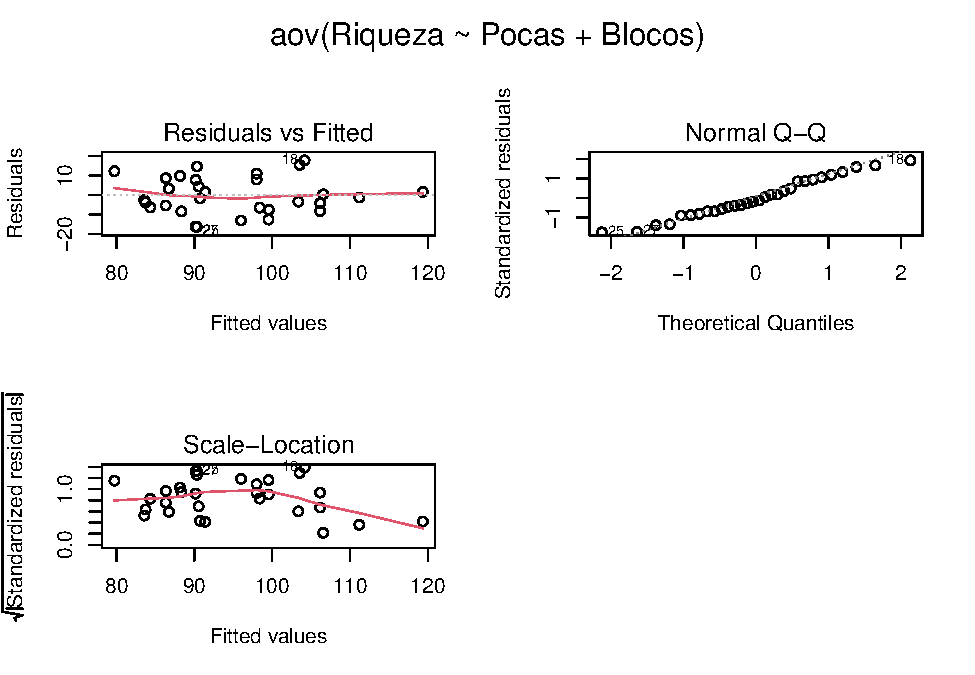
\includegraphics{livro_r_ecologia_files/figure-latex/unnamed-chunk-19-1.pdf}

\begin{Shaded}
\begin{Highlighting}[]
\KeywordTok{dev.off}\NormalTok{()}
\end{Highlighting}
\end{Shaded}

\begin{verbatim}
## null device 
##           1
\end{verbatim}

Percebam que o resultado da Anova (Pr(\textgreater F) \textless{} 0.001) indica que devemos rejeitar a hipótese nula que não há diferença entre as médias dos grupos. Contudo, os resultados não mostram quais são os grupos que apresentam diferenças. Para isso, temos que realizar testes de comparações múltiplas \emph{post-hoc} para detectar os grupos que apresentam diferenças significativas entre as médias. \textbf{Observação} Os testes \emph{post-hoc} só devem ser utilizados quando rejeitamos a hipótese nula (P \textless{} 0.05) no teste da Anova.

\begin{Shaded}
\begin{Highlighting}[]
\CommentTok{# Diferenças entre os tratamentos}
\CommentTok{#***********************************}
\CommentTok{# Teste de Tuckey's honest significant difference}
\KeywordTok{library}\NormalTok{(lsmeans)}
\KeywordTok{pairs}\NormalTok{(}\KeywordTok{lsmeans}\NormalTok{(model_bloco1, }\StringTok{"Pocas"}\NormalTok{), }\DataTypeTok{adjust =} \StringTok{"tukey"}\NormalTok{)}
\end{Highlighting}
\end{Shaded}

\begin{verbatim}
##  contrast                estimate   SE df t.ratio p.value
##  Borda - (Int-100m)        16.000 6.57 20  2.436  0.1463 
##  Borda - (Int-50m)         19.833 6.57 20  3.020  0.0472 
##  Borda - (Mat-100m)        15.833 6.57 20  2.411  0.1531 
##  Borda - (Mat-50m)          8.167 6.57 20  1.244  0.7269 
##  (Int-100m) - (Int-50m)     3.833 6.57 20  0.584  0.9760 
##  (Int-100m) - (Mat-100m)   -0.167 6.57 20 -0.025  1.0000 
##  (Int-100m) - (Mat-50m)    -7.833 6.57 20 -1.193  0.7553 
##  (Int-50m) - (Mat-100m)    -4.000 6.57 20 -0.609  0.9720 
##  (Int-50m) - (Mat-50m)    -11.667 6.57 20 -1.777  0.4135 
##  (Mat-100m) - (Mat-50m)    -7.667 6.57 20 -1.167  0.7692 
## 
## Results are averaged over the levels of: Blocos 
## P value adjustment: tukey method for comparing a family of 5 estimates
\end{verbatim}

Visualizar os resultados em gráfico

\begin{Shaded}
\begin{Highlighting}[]
\CommentTok{# Reordenando a ordem que os grupos irão aparecer no gráfico}
\NormalTok{dados_bloco}\OperatorTok{$}\NormalTok{Pocas <-}\StringTok{ }\KeywordTok{factor}\NormalTok{(dados_bloco}\OperatorTok{$}\NormalTok{Pocas, }
                              \DataTypeTok{levels=}\KeywordTok{c}\NormalTok{(}\StringTok{"Int-100m"}\NormalTok{, }\StringTok{"Int-50m"}\NormalTok{, }\StringTok{"Borda"}\NormalTok{, }\StringTok{"Mat-50m"}\NormalTok{, }\StringTok{"Mat-100m"}\NormalTok{))}

\CommentTok{# Gráfico}
\KeywordTok{library}\NormalTok{(ggplot2)}
\KeywordTok{ggplot}\NormalTok{(}\DataTypeTok{data =}\NormalTok{ dados_bloco, }\KeywordTok{aes}\NormalTok{(}\DataTypeTok{x=}\NormalTok{ Pocas, }\DataTypeTok{y=}\NormalTok{ Riqueza)) }\OperatorTok{+}\StringTok{ }
\StringTok{  }\KeywordTok{labs}\NormalTok{(}\DataTypeTok{x =} \StringTok{"Poças artificiais"}\NormalTok{, }\DataTypeTok{y =} \StringTok{"Riqueza de espécies de anuros"}\NormalTok{, }\DataTypeTok{size =} \DecValTok{20}\NormalTok{) }\OperatorTok{+}
\StringTok{  }\KeywordTok{geom_boxplot}\NormalTok{(}\DataTypeTok{color=}\StringTok{"black"}\NormalTok{, }\DataTypeTok{show.legend =} \OtherTok{FALSE}\NormalTok{,}
               \DataTypeTok{alpha =} \FloatTok{0.4}\NormalTok{) }\OperatorTok{+}
\StringTok{  }\KeywordTok{geom_jitter}\NormalTok{(}\DataTypeTok{shape =} \DecValTok{16}\NormalTok{, }\DataTypeTok{position=}\KeywordTok{position_jitter}\NormalTok{(}\FloatTok{0.1}\NormalTok{), }\DataTypeTok{cex =} \DecValTok{5}\NormalTok{, }\DataTypeTok{alpha =} \FloatTok{0.7}\NormalTok{) }\OperatorTok{+}
\StringTok{  }\KeywordTok{scale_x_discrete}\NormalTok{(}\DataTypeTok{labels=}\KeywordTok{c}\NormalTok{(}\StringTok{"-100m"}\NormalTok{,}\StringTok{"-50m"}\NormalTok{,}\StringTok{"Borda"}\NormalTok{, }\StringTok{"50m"}\NormalTok{, }\StringTok{"100m"}\NormalTok{)) }\OperatorTok{+}
\StringTok{  }\KeywordTok{theme}\NormalTok{(}\DataTypeTok{axis.title.y =} \KeywordTok{element_text}\NormalTok{(}\DataTypeTok{size =} \DecValTok{17}\NormalTok{), }\DataTypeTok{axis.title.x =} \KeywordTok{element_text}\NormalTok{(}\DataTypeTok{size =} \DecValTok{17}\NormalTok{)) }\OperatorTok{+}
\StringTok{  }\KeywordTok{theme}\NormalTok{(}\DataTypeTok{axis.text.y =} \KeywordTok{element_text}\NormalTok{(}\DataTypeTok{size =} \DecValTok{17}\NormalTok{), }\DataTypeTok{axis.text.x =} \KeywordTok{element_text}\NormalTok{(}\DataTypeTok{size =} \DecValTok{17}\NormalTok{)) }\OperatorTok{+}
\StringTok{  }\KeywordTok{theme}\NormalTok{(}\DataTypeTok{panel.border =} \KeywordTok{element_rect}\NormalTok{(}\DataTypeTok{colour =} \StringTok{"black"}\NormalTok{, }\DataTypeTok{fill=}\OtherTok{NA}\NormalTok{, }\DataTypeTok{size =} \DecValTok{2}\NormalTok{)) }
\end{Highlighting}
\end{Shaded}

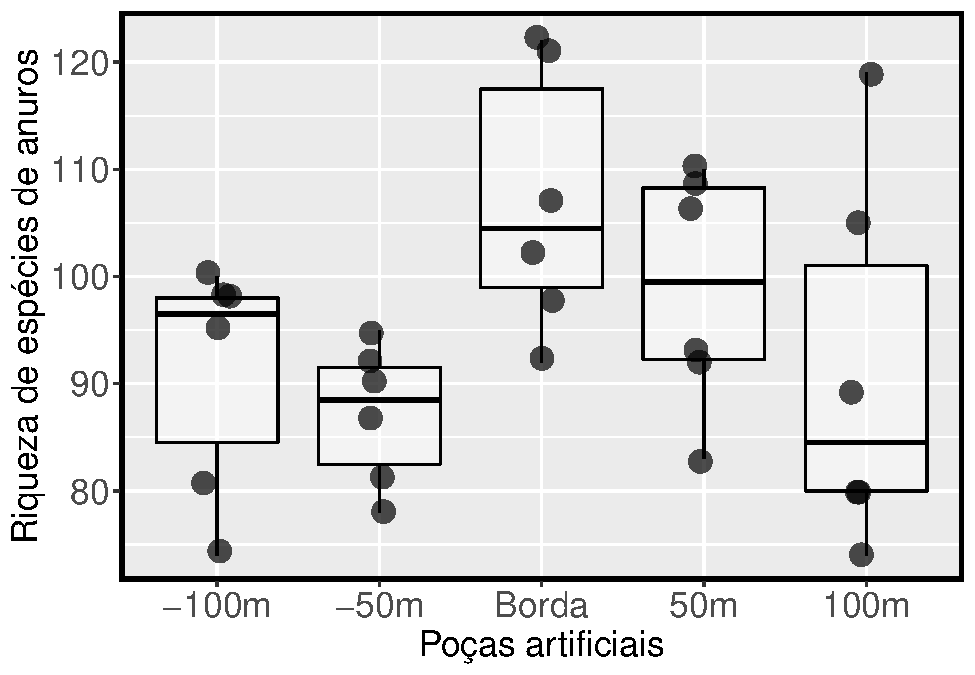
\includegraphics{livro_r_ecologia_files/figure-latex/unnamed-chunk-21-1.pdf}

\textbf{Interpretação dos resultados}

Neste exemplo, rejeitamos a hipótese nula que a distância da poças artificiais até as bordas dos fragmentos florestais não influência a riqueza de espécies de anuros. As poças artificiais instaladas nas bordas dos fragmentos florestais apresentaram maior riqueza de espécies do que as poças distantes.

~

\hypertarget{anuxe1lise-de-covariuxe2ncia-ancova}{%
\section{Análise de covariância (ANCOVA)}\label{anuxe1lise-de-covariuxe2ncia-ancova}}

A ANCOVA pode ser compreendida como uma extensão da Anova com a adição de variável contínua (covariável) medida em todas as unidades amostrais (Gotelli \& Ellison 2013). A ideia é que a covariável também afete os valores da variável resposta. Não incluir a covariável irá fazer com que a variação não explicada pelo modelo concentre-se nos resíduos. Incluindo a covariável, o tamanho do resíduo é menor, e o teste para avaliar as diferenças nos tratamentos terá mais poder estatístico.

~

\hypertarget{exemplo-pruxe1tico-1---ancova}{%
\subsubsection{Exemplo prático 1 - ANCOVA}\label{exemplo-pruxe1tico-1---ancova}}

\hypertarget{explicauxe7uxe3o-dos-dados-9}{%
\paragraph{Explicação dos dados}\label{explicauxe7uxe3o-dos-dados-9}}

Neste exemplo, avaliaremos o efeito da herbivoria na biomassa dos frutos de uma espécie de árvore na Mata Atlântica. O delineamento experimental permitiu que alguns indivíduos sofressem herbivoria e outros não. Os pesquisadores também mediram o tamanho da raiz dos indíviduos para inseri-la como uma covariável no modelo.

\textbf{Pergunta:}

\begin{quote}
A herbivoria diminiu a biomssa dos frutos?
\end{quote}

\textbf{Predições}

\begin{quote}
Os indivíduos que sofreram herbivoria irão produzir frutos com menor biomassa do que os indivíduos sem herbivoria.
\end{quote}

\textbf{Variáveis}

\begin{itemize}
\tightlist
\item
  Variáveis preditoras

  \begin{itemize}
  \tightlist
  \item
    Dataframe com as indivíduos da espéci de planta (unidade amostral) nas linhas e o tratamento e a covariável nas colunas.
  \end{itemize}
\end{itemize}

\textbf{Checklist}

\begin{itemize}
\tightlist
\item
  Verificar se o seu dataframe está com as unidades amostrais nas linhas e variáveis preditoras nas colunas.
\end{itemize}

\hypertarget{anuxe1lise-9}{%
\subsection{Análise}\label{anuxe1lise-9}}

Cálculo da ANCOVA

\begin{Shaded}
\begin{Highlighting}[]
\CommentTok{## IMPORTANDO DADOS}
\CommentTok{#********************}
\NormalTok{dados_ancova <-}\StringTok{ }\NormalTok{ecodados}\OperatorTok{::}\NormalTok{ancova}
\KeywordTok{str}\NormalTok{(dados_ancova) }\CommentTok{# verificar se o dataframe foi lido corretamente}
\end{Highlighting}
\end{Shaded}

\begin{verbatim}
## 'data.frame':	40 obs. of  3 variables:
##  $ Raiz      : num  6.22 6.49 4.92 5.13 5.42 ...
##  $ Biomassa  : num  59.8 61 14.7 19.3 34.2 ...
##  $ Herbivoria: chr  "Sem_herb" "Sem_herb" "Sem_herb" "Sem_herb" ...
\end{verbatim}

\begin{Shaded}
\begin{Highlighting}[]
\CommentTok{# ANALISE ANCOVA}
\CommentTok{#****************************************}
\NormalTok{modelo_ancova <-}\StringTok{ }\KeywordTok{lm}\NormalTok{(Biomassa }\OperatorTok{~}\StringTok{ }\NormalTok{Herbivoria }\OperatorTok{+}\StringTok{ }\NormalTok{Raiz, }\DataTypeTok{data =}\NormalTok{ dados_ancova)}

\CommentTok{# VERIFICANDO A NORMALIDADE E HOMOGENEIDADE DAS VARIÂNCIAS}
\CommentTok{#***********************************************************************}
\CommentTok{# Esta função mostra os resultados para multicolinearidade (a), dois gráficos avaliando a normalidade dos resíduos (b e  c), e um gráfico para a homogeneidade dos resíduos (d).}
\KeywordTok{library}\NormalTok{(sjPlot)}
\KeywordTok{plot_grid}\NormalTok{(}\KeywordTok{plot_model}\NormalTok{(modelo_ancova, }\DataTypeTok{type =} \StringTok{"diag"}\NormalTok{))}
\end{Highlighting}
\end{Shaded}

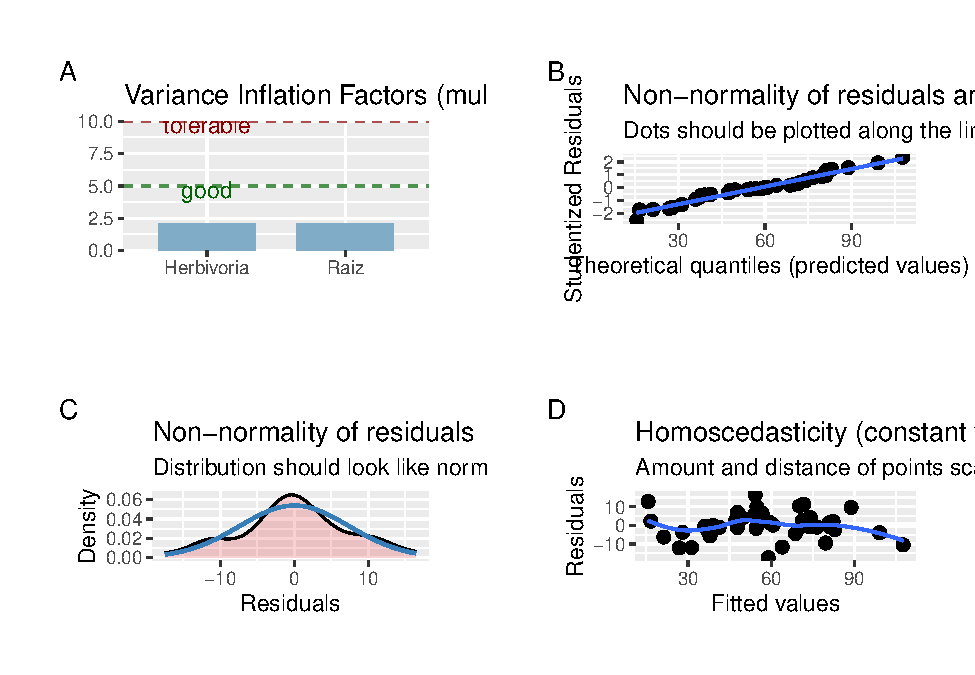
\includegraphics{livro_r_ecologia_files/figure-latex/unnamed-chunk-22-1.pdf}

\begin{Shaded}
\begin{Highlighting}[]
\CommentTok{# OLHANDO OS RESULTADOS}
\CommentTok{#********************}
\KeywordTok{anova}\NormalTok{(modelo_ancova)}
\end{Highlighting}
\end{Shaded}

\begin{verbatim}
## Analysis of Variance Table
## 
## Response: Biomassa
##            Df  Sum Sq Mean Sq F value    Pr(>F)    
## Herbivoria  1  1941.9  1941.9  33.759 1.135e-06 ***
## Raiz        1 17434.1 17434.1 303.075 < 2.2e-16 ***
## Residuals  37  2128.4    57.5                      
## ---
## Signif. codes:  0 '***' 0.001 '**' 0.01 '*' 0.05 '.' 0.1 ' ' 1
\end{verbatim}

Percebam que o resultado da ANCOVA (Pr(\textgreater F) \textless{} 0.001) indica que tanto a herbivoria como a o tamanho da raiz (covariável) tem efeitos significativos na biomassa dos frutos.

Visualizar os resultados em gráfico

\begin{Shaded}
\begin{Highlighting}[]
\CommentTok{# Gráfico}
\KeywordTok{library}\NormalTok{(ggplot2)}
\KeywordTok{ggplot}\NormalTok{(}\DataTypeTok{data =}\NormalTok{ dados_ancova, }\KeywordTok{aes}\NormalTok{(}\DataTypeTok{x=}\NormalTok{ Raiz, }\DataTypeTok{y=}\NormalTok{ Biomassa, }\DataTypeTok{fill =}\NormalTok{ Herbivoria)) }\OperatorTok{+}\StringTok{ }
\StringTok{  }\KeywordTok{labs}\NormalTok{(}\DataTypeTok{x =} \StringTok{"Tamanho da raiz (cm)"}\NormalTok{, }\DataTypeTok{y =} \StringTok{"Biomassa dos frutos (g)"}\NormalTok{, }\DataTypeTok{size =} \DecValTok{20}\NormalTok{) }\OperatorTok{+}
\StringTok{  }\KeywordTok{geom_point}\NormalTok{(}\DataTypeTok{size =} \DecValTok{15}\NormalTok{, }\DataTypeTok{shape =} \DecValTok{21}\NormalTok{) }\OperatorTok{+}
\StringTok{  }\KeywordTok{theme}\NormalTok{(}\DataTypeTok{axis.title.y =} \KeywordTok{element_text}\NormalTok{(}\DataTypeTok{size =} \DecValTok{17}\NormalTok{), }\DataTypeTok{axis.title.x =} \KeywordTok{element_text}\NormalTok{(}\DataTypeTok{size =} \DecValTok{17}\NormalTok{)) }\OperatorTok{+}
\StringTok{  }\KeywordTok{theme}\NormalTok{(}\DataTypeTok{axis.text.y =} \KeywordTok{element_text}\NormalTok{(}\DataTypeTok{size =} \DecValTok{17}\NormalTok{), }\DataTypeTok{axis.text.x =} \KeywordTok{element_text}\NormalTok{(}\DataTypeTok{size =} \DecValTok{17}\NormalTok{)) }\OperatorTok{+}
\StringTok{  }\KeywordTok{theme}\NormalTok{(}\DataTypeTok{panel.grid.major =} \KeywordTok{element_blank}\NormalTok{(),  }
        \DataTypeTok{panel.border =} \KeywordTok{element_rect}\NormalTok{(}\DataTypeTok{colour =} \StringTok{"black"}\NormalTok{, }\DataTypeTok{fill=}\OtherTok{NA}\NormalTok{, }\DataTypeTok{size =} \DecValTok{2}\NormalTok{)) }\OperatorTok{+}
\StringTok{  }\KeywordTok{theme}\NormalTok{(}\DataTypeTok{legend.position=}\StringTok{"bottom"}\NormalTok{) }\OperatorTok{+}
\StringTok{  }\KeywordTok{scale_fill_discrete}\NormalTok{(}\DataTypeTok{name =} \StringTok{"Herbivoria"}\NormalTok{, }\DataTypeTok{labels =} \KeywordTok{c}\NormalTok{(}\StringTok{"Com herbivoria"}\NormalTok{, }\StringTok{"Sem herbivoria"}\NormalTok{)) }\OperatorTok{+}
\StringTok{  }\KeywordTok{geom_smooth}\NormalTok{(}\KeywordTok{aes}\NormalTok{(}\DataTypeTok{color=}\NormalTok{Herbivoria), }\DataTypeTok{method=}\StringTok{"lm"}\NormalTok{, }\DataTypeTok{show.legend =} \OtherTok{FALSE}\NormalTok{)}
\end{Highlighting}
\end{Shaded}

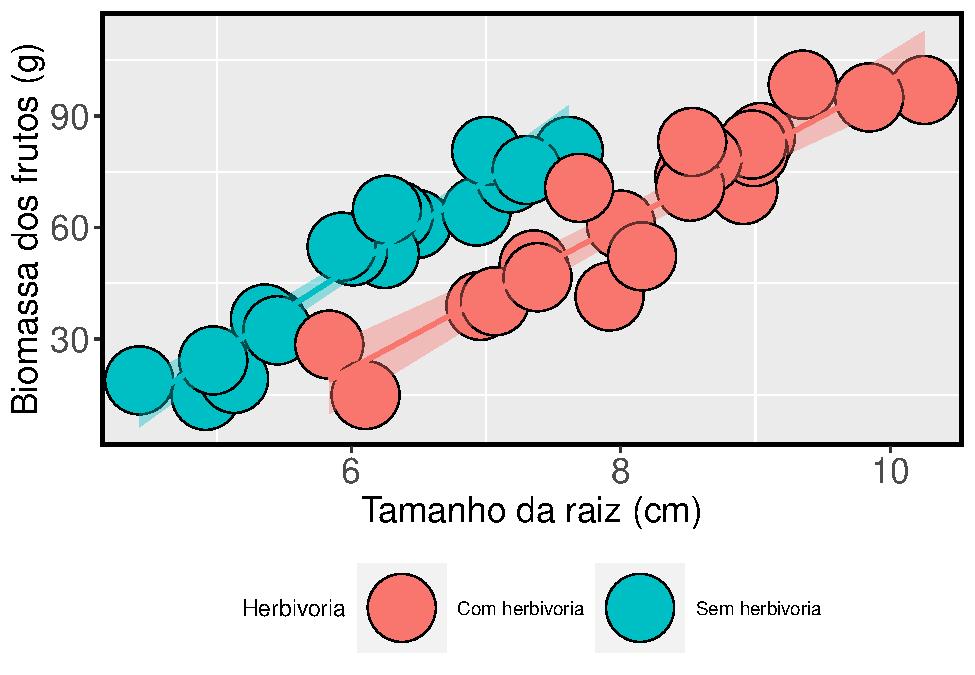
\includegraphics{livro_r_ecologia_files/figure-latex/unnamed-chunk-23-1.pdf}

\textbf{Interpretação dos resultados}

Neste exemplo, o tamanho da raiz (covariável) tem uma relação positiva com a biomassa dos frutos. Quanto maior o tamanho da raiz, maior a biomassa dos frutos. Usando a ANCOVA e controlando o efeito da covariável, percebemos que a herbivoria também afeta a biomassa dos frutos. Os indivíduos que não sofreram herbivoria produziram frutos com maior biomassa do que os indivíduos com herbivoria.

~

\hypertarget{para-se-aprofundar}{%
\subsection{Para se aprofundar}\label{para-se-aprofundar}}

\begin{itemize}
\tightlist
\item
  Recomendamos aos interessados os livros: i) Zar (2010) Biostatiscal analysis; ii) Gotelli \& Ellison (2013) A primer of ecological statistics; e iii) Quinn \& Keough (2002) Experimental design and data analysis for biologists.
\end{itemize}

\hypertarget{introduuxe7uxe3o-uxe0-anuxe1lises-multidimensionais}{%
\chapter{Introdução à Análises Multidimensionais}\label{introduuxe7uxe3o-uxe0-anuxe1lises-multidimensionais}}

Neste módulo iremos aprender como implementar no R as análises multivariadas mais comumente utilizadas em ecologia de comunidades. Para isso precisaremos dos pacotes \texttt{vegan},\texttt{labdsv} e \texttt{ade4}. Procuraremos explicar brevemente a lógica por trás de cada teste, a sua aplicação em problemas comumente encontrados em estudos ecológicos, mas não destrinchar detalhadamente como cada método funciona e o seu componente matemático.

Em geral, análises multivariadas têm três principais utilidades: reduzir a dimensionalidade dos dados e encontrar a principal direção de variação dos dados, testar relações entre matrizes, ou ainda encontrar diferenças entre grupos. Apesar dessas análises também serem utilizadas como análises exploratórias e para descrever padrões em estudos ecológicos, a necessidade de se ter hipóteses, ou ao menos expectativas a priori, não pode ser ignorada. Se quiser saber mais sobre aspectos teóricos e filosóficos das análises, sugerimos consultar James \& McCulloch (1990). Antes de entrar de cabeça nas análises multivariadas também, sugerimos fortemente o estudo de métodos de amostragem e como fazer boas perguntas. Não vamos nos extender muito nesses tópicos porque eles foram abordados nas aulas disponíveis no \href{https://www.youtube.com/playlist?list=PLy2rjqiD2VP5G6pqMo_QlWo7I3yu-uFTk}{YouTube}.

Análises multivariadas podem ser divididas, grosseiramente, em dois tipos: agrupamento e ordenação. Análises de agrupamento em geral tentam agrupar objetos (observações) em grupos de maneira que objetos do mesmo grupo sejam mais semelhantes entre si do que objetos de outros grupos. Mais formalmente, o agrupamento de objetos (ou descritores) é uma operação pela qual um conjunto de objetos (ou descritores) é particionado em dois ou mais subconjuntos, usando regras pré-estabelecidas de aglomeração ou divisão (Legendre \& Legendre, 2012). Por outro lado, a análise de ordenação é uma operação pela qual os objetos (ou descritores) são posicionados num espaço que contém menos dimensões que o conjunto de dados original; a posição dos objetos ou descritores em relação aos outros também podem ser usadas para agrupá-los.

Vamos começar com análises de agrupamento. Aqui vamos exemplificar dois métodos: uma técnica de agrupamento hierarquica (dendrograma) e outra não-hierarquica (k-means.

\hypertarget{backgorund-da-anuxe1lise}{%
\section{Backgorund da análise}\label{backgorund-da-anuxe1lise}}

O objetivo da análise de agrupamento é agrupar objetos admitindo que haja um grau de similaridade entre eles. Esta análise pode ser utilizada ainda para classificar uma população em grupos homogêneos de acordo com uma característica de interesse. A grosso modo, uma análise de agrupamento tenta resumir uma grande quantidade de dados e apresentála de maneira fácil de visualizar e entender (em geral, na forma de um dendrograma). No entanto, os resultados da análise podem não refletir necessariamente toda a informação originalmente contida na matriz de dados. Para avaliar o quão bem uma análise de agrupamento representa os dados originais existe uma métrica --- o coeficiente de correlação cofenético --- o qual discutiremos em detalhes mais adiante.

Antes de considerar algum método de agrupamento, pense porque você esperaria que houvesse uma descontinuidade nos dados; ou ainda, considere se existe algum ganho prático em dividir uma nuvem de objetos contínuos em grupos. O padrão apresentado pelo dendograma depende do protocolo utilizado (método de agrupamento e índice de dissimilaridade); os grupos formados dependem do nível de corte escolhido. O leitor interessado é remetido à duas referências: Legendre \& Legendre (2012) e Borcard et al.~(2018).

\hypertarget{exemplo-1}{%
\section{Exemplo 1:}\label{exemplo-1}}

\textbf{Pergunta:}

\begin{quote}
Existem grupos de espécies de anfíbios anuros com padrões de ocorrência similar ao longo de poças?
\end{quote}

\textbf{Predições}

\begin{quote}
\begin{itemize}
\tightlist
\item
  1: Iremos encontrar ao menos dois grupos de espécies: aquelas que ocorrem em poças dentro de floresta vs.~aquelas que ocorrem em poças de áreas abertas.
\end{itemize}
\end{quote}

\textbf{Variáveis}

\begin{itemize}
\tightlist
\item
  Variáveis preditoras

  \begin{itemize}
  \item
    \begin{enumerate}
    \def\labelenumi{\arabic{enumi}.}
    \tightlist
    \item
      A nossa matriz de dados contém a abundância das espécies nas linhas e locais (poças) nas colunas.
    \end{enumerate}
  \end{itemize}
\end{itemize}

\hypertarget{explicauxe7uxe3o-da-anuxe1lise}{%
\subsection{Explicação da análise}\label{explicauxe7uxe3o-da-anuxe1lise}}

A matriz deve conter os objetos a serem agrupados (e.g., espécies) nas linhas e as variáveis (e.g., locais de coleta ou medidas morfológicas) nas colunas.
A escolha do método de agrupamento é crítico para a escolha de um coeficiente de associação. É importante compreender as propriedades dos métodos de agrupamento para interpretar corretamente a estrutura ecológica que eles evidenciam (Legendre \& Legendre, 2012). De acordo com a classificação de Sneath \& Sokal (1973) existem cinco tipos de métodos: 1) seqüenciais ou simultâneos; 2) aglomerativo ou divisivo ;3) monotéticos ou politéticos; 4) hierárquico ou não hierárquicos e 5) probabilístico.

Métodos hierárquicos podem ser divididos naqueles que consideram o centróide ou amédia aritmética entre os grupos. O principal método hierárquico que utiliza a média aritmética é o UPGMA (Agrupamento pelas médias aritméticas não ponderadas), e o principal método que utiliza centróides é a Distância mínima de Ward.

O UPGMA funciona da seguinte forma: a maior similaridade (ou menor distância) identifica os próximos agrupamentos a serem formados. Após esse evento, o método calcula a média aritmética das similaridades ou distâncias entre um objeto e cada um dos membros do grupo ou, no caso de um grupo previamente formado, entre todos os membros dos dois grupos. Todos os objetos recebem pesos iguais no cálculo.

O método de Ward é baseado no critério de quadrados mínimos (OLS), o mesmo utilizado para ajustar um modelo linear. O objetivo é definir os grupos de maneira que a soma de quadrados (i.e.~similar ao erro quadrado da ANOVA) dentro dos grupos seja minimizada (Borcard et al.~2018).

\textbf{Checklist}

\begin{itemize}
\tightlist
\item
  Verifique se não há espaço nos nomes das colunas e linhas
\item
  Se os dados forem de abundância, recomenda-se realizar a transformação de Hellinger (Legendre \& Gallagher, 2001).
\item
  Se a matriz original contiver muitos valores discrepantes (e.g., uma espécie muito mais ou muito menos abundante que outras) é necessário transformar os dados usando \texttt{log1p}.
\item
  Se as variáveis forem medidas tomadas em diferentes escalas (metros, graus celcius etc), é necessário padronizar cada variável para ter a média 0 e desvio padrão 1. Isso pode ser feito utulizando a função \texttt{decostand} do pacote \texttt{vegan}.
\end{itemize}

\hypertarget{anuxe1lise}{%
\subsection{Análise}\label{anuxe1lise}}

Para começar, vamos primeiro importar os dados e depois calcular a matriz de distância que seja adequada para o tipo de dado que temos (abundância de espécies - dados de contagem)

\begin{Shaded}
\begin{Highlighting}[]
\KeywordTok{library}\NormalTok{(ecodados) }\CommentTok{# Carrega o arquivo multivar_bocaina}
\KeywordTok{library}\NormalTok{(vegan)}


\CommentTok{#sp_compos <- read.table("bocaina.txt", h=TRUE)}
\NormalTok{sp_compos  <-}\StringTok{ }\NormalTok{multivar_bocaina}
\KeywordTok{head}\NormalTok{(sp_compos)}
\end{Highlighting}
\end{Shaded}

\begin{verbatim}
##         BP4  PP4 PP3  AP1 AP2 PP1 PP2 BP9  PT1 PT2 PT3 BP2 PT5
## Aper      0    3   0    0   2   0   0   0    0   0   0 181   0
## Bahe    859   14  14    0  87 312 624 641    0   0   0  14   0
## Rict   1772 1517 207  573 796   0   0   0    0   0   0   0   0
## Cleuco    0    0   0    0   0   0   0   0    0  29 369   0  84
## Dmic      0    0   6   60   4   0   0   0 2758 319  25   0 329
## Dmin      0   84 344 1045  90   0   0   0    8   0   0   0   0
\end{verbatim}

\begin{Shaded}
\begin{Highlighting}[]
\NormalTok{bocaina <-}\StringTok{ }\KeywordTok{t}\NormalTok{(sp_compos)}\CommentTok{#transpondo a matriz para obter a classificação por linhas}
\NormalTok{distBocaina <-}\StringTok{ }\KeywordTok{vegdist}\NormalTok{(bocaina, }\DataTypeTok{method=}\StringTok{"horn"}\NormalTok{)}\CommentTok{#produz uma matriz de similaridade com o coeficiente de Morisita-Horn}
\NormalTok{dendro <-}\StringTok{ }\KeywordTok{hclust}\NormalTok{(distBocaina, }\DataTypeTok{method=}\StringTok{"average"}\NormalTok{)}\CommentTok{#produz um agrupamento com a função hclust e o método UPGMA}
\end{Highlighting}
\end{Shaded}

Visualizar os resultados

\begin{Shaded}
\begin{Highlighting}[]
\KeywordTok{plot}\NormalTok{(dendro)}
\end{Highlighting}
\end{Shaded}

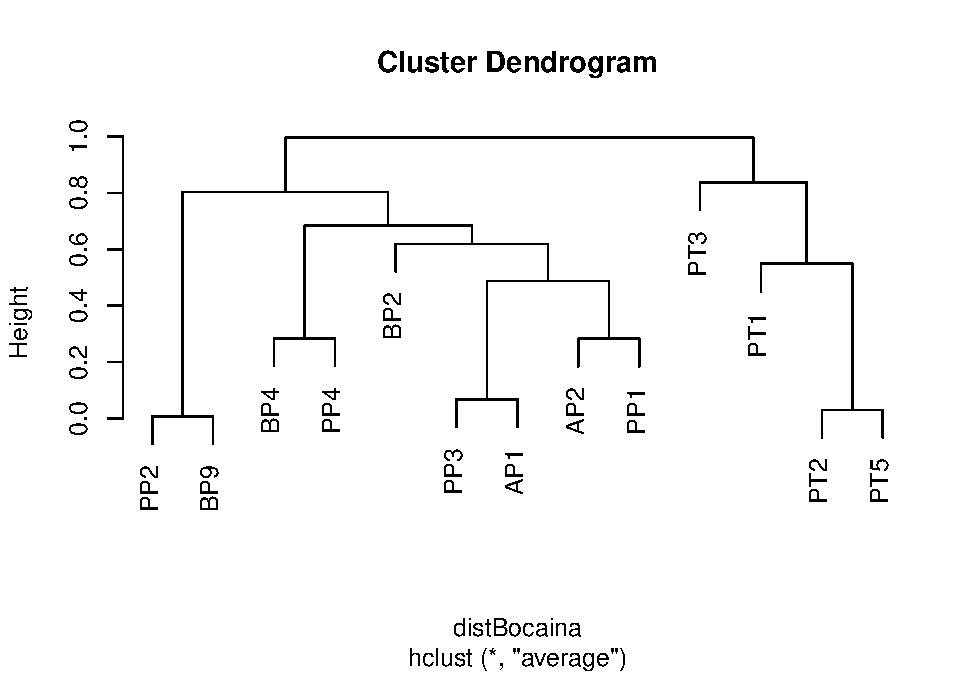
\includegraphics{livro_r_ecologia_files/figure-latex/unnamed-chunk-25-1.pdf}

\hypertarget{interpretauxe7uxe3o-dos-resultados}{%
\subsubsection{Interpretação dos resultados}\label{interpretauxe7uxe3o-dos-resultados}}

Antes de começarmos a interpretar os resultados precisamos verificar que o agrupamento reduziu a dimensionalidade da matiz de forma eficiente, de maneira a não distorcer a informação. Fazemos isso calculando o \textbf{Coeficiente de correlação cofenética (CCC)}

\begin{Shaded}
\begin{Highlighting}[]
\NormalTok{cofresult <-}\StringTok{ }\KeywordTok{cophenetic}\NormalTok{(dendro)}
\KeywordTok{cor}\NormalTok{(cofresult, distBocaina)}
\end{Highlighting}
\end{Shaded}

\begin{verbatim}
## [1] 0.8819701
\end{verbatim}

Um CCC \textgreater{} .7 indica uma boa representação. Portanto, o nosso resultado de 0.8819701 é bastante alto, garantindo que o dendrograma é adequado.

No entanto, para interpretar os resultados precisamos antes definir um nível de corte, que vai nos dizer quantos grupos existem. Há vários métodos para definir grupos, desde os heurísticos aos que utilizam bootstrap. Se quisermos interpretar este dendrograma, podemos por exemplo estabelecer um nível de corte de 50\% de distância (ou seja, grupos cujos objetos tenham ao menos 50\% de similaridade entre si).

\begin{Shaded}
\begin{Highlighting}[]
\KeywordTok{plot}\NormalTok{(dendro)}
\NormalTok{k =}\StringTok{ }\DecValTok{4}
\NormalTok{n =}\StringTok{ }\KeywordTok{nrow}\NormalTok{(bocaina)}
\NormalTok{MidPoint =}\StringTok{ }\NormalTok{(dendro}\OperatorTok{$}\NormalTok{height[n}\OperatorTok{-}\NormalTok{k] }\OperatorTok{+}\StringTok{ }\NormalTok{dendro}\OperatorTok{$}\NormalTok{height[n}\OperatorTok{-}\NormalTok{k}\OperatorTok{+}\DecValTok{1}\NormalTok{]) }\OperatorTok{/}\StringTok{ }\DecValTok{2}
\KeywordTok{abline}\NormalTok{(}\DataTypeTok{h =}\NormalTok{ MidPoint, }\DataTypeTok{lty=}\DecValTok{2}\NormalTok{)}
\end{Highlighting}
\end{Shaded}

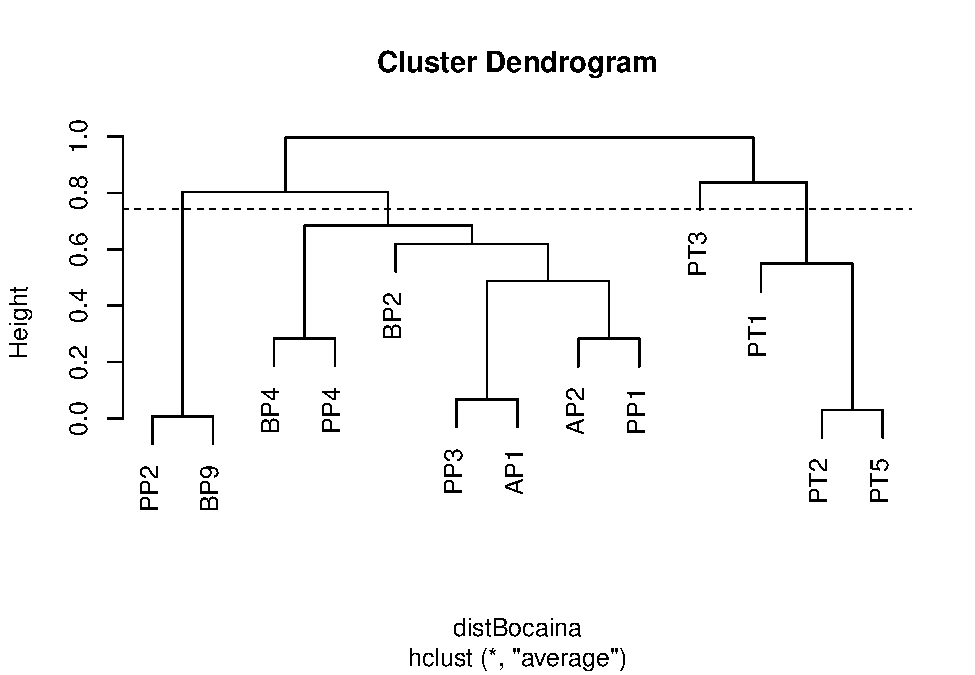
\includegraphics{livro_r_ecologia_files/figure-latex/unnamed-chunk-27-1.pdf}

Nesse caso teremos a formação de cinco grupos, representados pelos nós que estão abaixo da linha de corte.

\hypertarget{exemplo-2}{%
\section{Exemplo 2:}\label{exemplo-2}}

A seguir, vamos utilizar o pacote \texttt{pvclust} que calcula automaticamente o nível de corte de similaridade baseado no Bootstrap de cada nó. Uma desvantagem deste método é que ele somente aceita índices de similaridade da função \texttt{dist} que possui apenas a distância Euclidiana, Manhattan e Canberra. Uma maneira de contornarmos essa limitação é utilizar transformações dos dados disponíveis na função \texttt{disttransform} no pacote \texttt{BiodiversityR} ou o \texttt{decostand} do pacote \texttt{vegan}. Também é possível utilizar a transformação de Box-Cox para dados multivariados, disponível no material suplementar de Legendre \& Borcard (2018) \href{http://www.ecography.org/appendix/ecog-03498}{aqui}

\begin{Shaded}
\begin{Highlighting}[]
\KeywordTok{library}\NormalTok{(pvclust)}
\KeywordTok{library}\NormalTok{(BiodiversityR)}
\end{Highlighting}
\end{Shaded}

Aqui vamos utilizar a distância de Chord para calcular a matriz de distância. Se transformarmos uma matriz usando a transformação Chord e depois calcularmos a distância Euclidiana, isso equivale à calcular diretamente a distância de Chord:

\begin{Shaded}
\begin{Highlighting}[]
\NormalTok{bocaina_transf <-}\StringTok{ }\KeywordTok{disttransform}\NormalTok{(bocaina, }\StringTok{"chord"}\NormalTok{)}
\NormalTok{analise <-}\StringTok{ }\KeywordTok{pvclust}\NormalTok{(bocaina_transf, }\DataTypeTok{method.hclust=}\StringTok{"average"}\NormalTok{, }\DataTypeTok{method.dist=}\StringTok{"euclidean"}\NormalTok{) }
\end{Highlighting}
\end{Shaded}

\begin{verbatim}
## Bootstrap (r = 0.46)... Done.
## Bootstrap (r = 0.54)... Done.
## Bootstrap (r = 0.69)... Done.
## Bootstrap (r = 0.77)... Done.
## Bootstrap (r = 0.85)... Done.
## Bootstrap (r = 1.0)... Done.
## Bootstrap (r = 1.08)... Done.
## Bootstrap (r = 1.15)... Done.
## Bootstrap (r = 1.23)... Done.
## Bootstrap (r = 1.38)... Done.
\end{verbatim}

\begin{Shaded}
\begin{Highlighting}[]
\KeywordTok{plot}\NormalTok{(analise, }\DataTypeTok{hang=}\OperatorTok{-}\DecValTok{1}\NormalTok{)}
\KeywordTok{pvrect}\NormalTok{(analise)}
\end{Highlighting}
\end{Shaded}

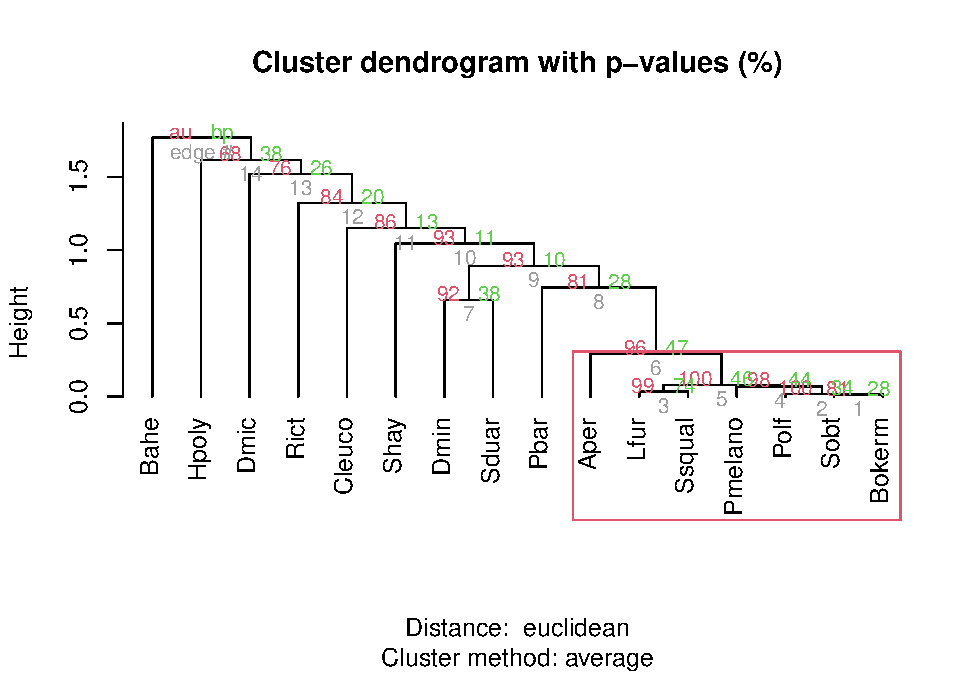
\includegraphics{livro_r_ecologia_files/figure-latex/unnamed-chunk-29-1.pdf}

É possível notar que existe um único grupo com BS \textgreater{} 95\%. Agora vamos tentar usar a distância de Hellinger:

\begin{Shaded}
\begin{Highlighting}[]
\NormalTok{bocaina_transf2 <-}\StringTok{ }\KeywordTok{disttransform}\NormalTok{(bocaina, }\StringTok{"hellinger"}\NormalTok{)}
\NormalTok{analise2 <-}\StringTok{ }\KeywordTok{pvclust}\NormalTok{(bocaina_transf2, }\DataTypeTok{method.hclust=}\StringTok{"average"}\NormalTok{, }\DataTypeTok{method.dist=}\StringTok{"euclidean"}\NormalTok{) }
\end{Highlighting}
\end{Shaded}

\begin{verbatim}
## Bootstrap (r = 0.46)... Done.
## Bootstrap (r = 0.54)... Done.
## Bootstrap (r = 0.69)... Done.
## Bootstrap (r = 0.77)... Done.
## Bootstrap (r = 0.85)... Done.
## Bootstrap (r = 1.0)... Done.
## Bootstrap (r = 1.08)... Done.
## Bootstrap (r = 1.15)... Done.
## Bootstrap (r = 1.23)... Done.
## Bootstrap (r = 1.38)... Done.
\end{verbatim}

\begin{Shaded}
\begin{Highlighting}[]
\KeywordTok{plot}\NormalTok{(analise2, }\DataTypeTok{hang=}\OperatorTok{-}\DecValTok{1}\NormalTok{)}
\KeywordTok{pvrect}\NormalTok{(analise2)}
\end{Highlighting}
\end{Shaded}

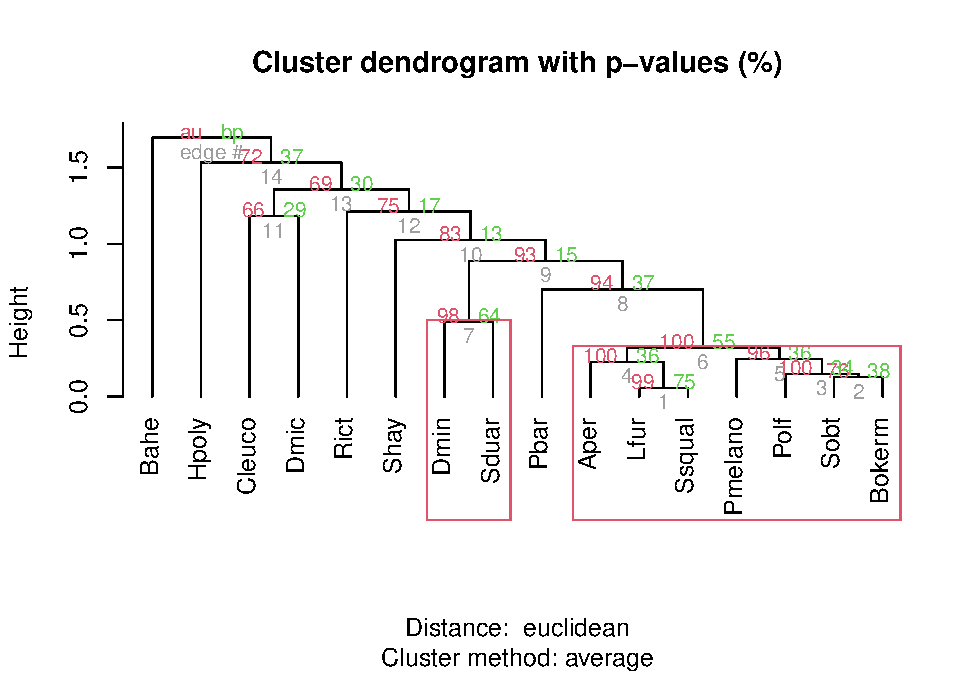
\includegraphics{livro_r_ecologia_files/figure-latex/unnamed-chunk-30-1.pdf}

Notem que se mudarmos o coeficiente de associação, o resultado também muda. Agora temos 1 grupo a mais, composto por \emph{Dendropsophus minutus} e \emph{Scinax duartei} que não apareciam antes. Isso se deve ao fato de que a distância de Hellinger dá menos peso para espécies raras do que a Chord.

\hypertarget{k-means-e-agrupamentos-nuxe3o-hierarquicos}{%
\chapter{K-means e agrupamentos não-hierarquicos}\label{k-means-e-agrupamentos-nuxe3o-hierarquicos}}

\hypertarget{backgorund-da-anuxe1lise-1}{%
\section{Backgorund da análise}\label{backgorund-da-anuxe1lise-1}}

K-means é um tipo de agrupamento não hierarquico porque não busca obter grupos menores que por sua vez pertencem a grupos maiores. Resumidamente, podemos calcular o K-means apartir de uma matriz quadrada ou de distância. Essa técnica procura particionar os objetos em \emph{k} grupos de maneira a minimizar a soma de quadrados entre grupos e maximizá-la dentro dos grupos. Um critério similar ao de uma ANOVA.

\hypertarget{exemplo-1-1}{%
\section{Exemplo 1:}\label{exemplo-1-1}}

\textbf{Pergunta:}

\begin{quote}
Qual é o número de grupos que melhor sumariza o padrão de ocorrência de espécies de peixes ao longo de um riacho?
\end{quote}

\textbf{Predições}

\begin{quote}
\begin{itemize}
\tightlist
\item
  1: O agrupamento ideal para explicar a variância no padrão de ocorrência de espécies é 4.
\end{itemize}
\end{quote}

\textbf{Variáveis}

\begin{itemize}
\tightlist
\item
  Variáveis resposta

  \begin{itemize}
  \item
    \begin{enumerate}
    \def\labelenumi{\arabic{enumi}.}
    \tightlist
    \item
      Para este exemplo iremos utilizar um conjunto de dados disponível no pacote \texttt{ade4} que contém dados de 27 espécies de peixes coletados em 30 pontos ao longo do Rio Doubs, na fronteira entre a França e Suiça.
    \end{enumerate}
  \end{itemize}
\end{itemize}

\hypertarget{explicauxe7uxe3o-da-anuxe1lise-1}{%
\subsection{Explicação da análise}\label{explicauxe7uxe3o-da-anuxe1lise-1}}

Um diferencial do K-means em relação aos agrupamentos hierarquicos (=clusters) é que o usuário pode escolher antecipadamente o número de grupos que quer formar.

\textbf{Checklist}

\begin{itemize}
\tightlist
\item
  Vamos normalizar os dados de abundância antes de entrar na análise propriamente, já que existem muitos zeros na matriz.
\end{itemize}

\hypertarget{anuxe1lise-1}{%
\subsection{Análise}\label{anuxe1lise-1}}

\begin{Shaded}
\begin{Highlighting}[]
\KeywordTok{library}\NormalTok{(ade4)}
\KeywordTok{data}\NormalTok{(doubs)}
\KeywordTok{head}\NormalTok{(doubs}\OperatorTok{$}\NormalTok{fish)}
\end{Highlighting}
\end{Shaded}

\begin{verbatim}
##   Cogo Satr Phph Neba Thth Teso Chna Chto Lele Lece Baba Spbi Gogo Eslu Pefl
## 1    0    3    0    0    0    0    0    0    0    0    0    0    0    0    0
## 2    0    5    4    3    0    0    0    0    0    0    0    0    0    0    0
## 3    0    5    5    5    0    0    0    0    0    0    0    0    0    1    0
## 4    0    4    5    5    0    0    0    0    0    1    0    0    1    2    2
## 5    0    2    3    2    0    0    0    0    5    2    0    0    2    4    4
## 6    0    3    4    5    0    0    0    0    1    2    0    0    1    1    1
##   Rham Legi Scer Cyca Titi Abbr Icme Acce Ruru Blbj Alal Anan
## 1    0    0    0    0    0    0    0    0    0    0    0    0
## 2    0    0    0    0    0    0    0    0    0    0    0    0
## 3    0    0    0    0    0    0    0    0    0    0    0    0
## 4    0    0    0    0    1    0    0    0    0    0    0    0
## 5    0    0    2    0    3    0    0    0    5    0    0    0
## 6    0    0    0    0    2    0    0    0    1    0    0    0
\end{verbatim}

\begin{Shaded}
\begin{Highlighting}[]
\NormalTok{spe <-}\StringTok{ }\NormalTok{doubs}\OperatorTok{$}\NormalTok{fish[}\OperatorTok{-}\DecValTok{8}\NormalTok{,]}\CommentTok{# retiro a linha 8, pois não há dados}
\NormalTok{spe.norm <-}\StringTok{ }\KeywordTok{decostand}\NormalTok{(spe, }\StringTok{"normalize"}\NormalTok{) }\CommentTok{# função do pacote vegan, ela faz várias padronizações, aqui ele normaliza  }
\end{Highlighting}
\end{Shaded}

O argumento \texttt{centers} na função abaixo indica o número de grupos que se quer formar. Neste exemplo estamos utilizando \texttt{centers=4}.

\begin{Shaded}
\begin{Highlighting}[]
\NormalTok{spe.kmeans <-}\StringTok{ }\KeywordTok{kmeans}\NormalTok{(spe.norm, }\DataTypeTok{centers=}\DecValTok{4}\NormalTok{, }\DataTypeTok{nstart=}\DecValTok{100}\NormalTok{)}
\NormalTok{spe.kmeans}
\end{Highlighting}
\end{Shaded}

\begin{verbatim}
## K-means clustering with 4 clusters of sizes 12, 6, 3, 8
## 
## Cluster means:
##         Cogo        Satr       Phph       Neba        Thth        Teso
## 1 0.10380209 0.542300691 0.50086515 0.43325916 0.114024105 0.075651573
## 2 0.06167791 0.122088022 0.26993915 0.35942538 0.032664966 0.135403325
## 3 0.00000000 0.000000000 0.00000000 0.00000000 0.000000000 0.000000000
## 4 0.00000000 0.006691097 0.02506109 0.06987391 0.006691097 0.006691097
##         Chna       Chto       Lele      Lece       Baba      Spbi       Gogo
## 1 0.00000000 0.00000000 0.06983991 0.1237394 0.02385019 0.0000000 0.05670453
## 2 0.06212775 0.21568957 0.25887226 0.2722562 0.15647062 0.1574388 0.16822286
## 3 0.05205792 0.00000000 0.07647191 0.3166705 0.00000000 0.0000000 0.20500174
## 4 0.10687104 0.09377516 0.14194394 0.2011411 0.24327992 0.1326062 0.28386032
##         Eslu       Pefl      Rham       Legi       Scer       Cyca       Titi
## 1 0.04722294 0.02949244 0.0000000 0.00000000 0.00000000 0.00000000 0.03833408
## 2 0.12276089 0.17261621 0.0793181 0.06190283 0.04516042 0.06190283 0.14539027
## 3 0.07647191 0.00000000 0.0000000 0.05205792 0.07647191 0.00000000 0.00000000
## 4 0.20630360 0.16920496 0.2214275 0.19066542 0.13171275 0.16019126 0.26230024
##         Abbr      Icme       Acce       Ruru       Blbj      Alal       Anan
## 1 0.00000000 0.0000000 0.00000000 0.01049901 0.00000000 0.0000000 0.00000000
## 2 0.01473139 0.0000000 0.03192175 0.32201597 0.01473139 0.1095241 0.04739636
## 3 0.00000000 0.0000000 0.18058775 0.31667052 0.05205792 0.7618709 0.00000000
## 4 0.19561641 0.1331835 0.26713081 0.32103755 0.22883055 0.3326939 0.18873077
## 
## Clustering vector:
##  1  2  3  4  5  6  7  9 10 11 12 13 14 15 16 17 18 19 20 21 22 23 24 25 26 27 
##  1  1  1  1  2  1  1  2  1  1  1  1  1  1  2  2  2  2  4  4  4  3  3  3  4  4 
## 28 29 30 
##  4  4  4 
## 
## Within cluster sum of squares by cluster:
## [1] 2.5101386 1.7361453 0.3560423 0.4696535
##  (between_SS / total_SS =  66.7 %)
## 
## Available components:
## 
## [1] "cluster"      "centers"      "totss"        "withinss"     "tot.withinss"
## [6] "betweenss"    "size"         "iter"         "ifault"
\end{verbatim}

O objeto que fornece o resultado contém: 1) o tamanho (número de objetos) em cada um dos 4 grupos; 2) o centroid de cada grupo e o pertencimento de cada espécie a cada grupo; e 3) o quando da Soma de Quadrados dos dados é explicada por esta conformação de grupos.

No entanto, não é possível saber a priori qual o número \emph{ideal} de grupos. Para descobrir isso repetimos o k-means com uma série de valores de \textbf{K}. Isso pode ser feito na função \texttt{cascadeKM}.

\begin{Shaded}
\begin{Highlighting}[]
\NormalTok{spe.KM.cascade <-}\StringTok{ }\KeywordTok{cascadeKM}\NormalTok{(spe.norm, }\DataTypeTok{inf.gr=}\DecValTok{2}\NormalTok{, }\DataTypeTok{sup.gr=}\DecValTok{10}\NormalTok{, }\DataTypeTok{iter=}\DecValTok{100}\NormalTok{, }\DataTypeTok{criterion=}\StringTok{"ssi"}\NormalTok{) }
\end{Highlighting}
\end{Shaded}

Tanto \textbf{calinski} quando \textbf{ssi} são bons critérios para encontrar o número ideal de grupos. Quanto maior o valor de \textbf{ssi} melhor (veja \texttt{?cascadeKM} mais detalhes).

\begin{Shaded}
\begin{Highlighting}[]
\CommentTok{# summary}
\NormalTok{spe.KM.cascade}\OperatorTok{$}\NormalTok{results}
\end{Highlighting}
\end{Shaded}

\begin{verbatim}
##      2 groups  3 groups  4 groups   5 groups   6 groups   7 groups  8 groups
## SSE 8.2149405 6.4768108 5.0719796 4.30155732 3.58561200 2.95236670 2.4840549
## ssi 0.1312111 0.1675852 0.1409061 0.05927008 0.07398577 0.08003379 0.0739309
##      9 groups 10 groups
## SSE 2.0521888  1.759929
## ssi 0.1446301  0.110006
\end{verbatim}

SSE: critério utilizado pelo algorítimo para achar o agrupamento ótimo dos objetos.

\begin{Shaded}
\begin{Highlighting}[]
\KeywordTok{plot}\NormalTok{(spe.KM.cascade, }\DataTypeTok{sortg=}\OtherTok{TRUE}\NormalTok{)}
\end{Highlighting}
\end{Shaded}

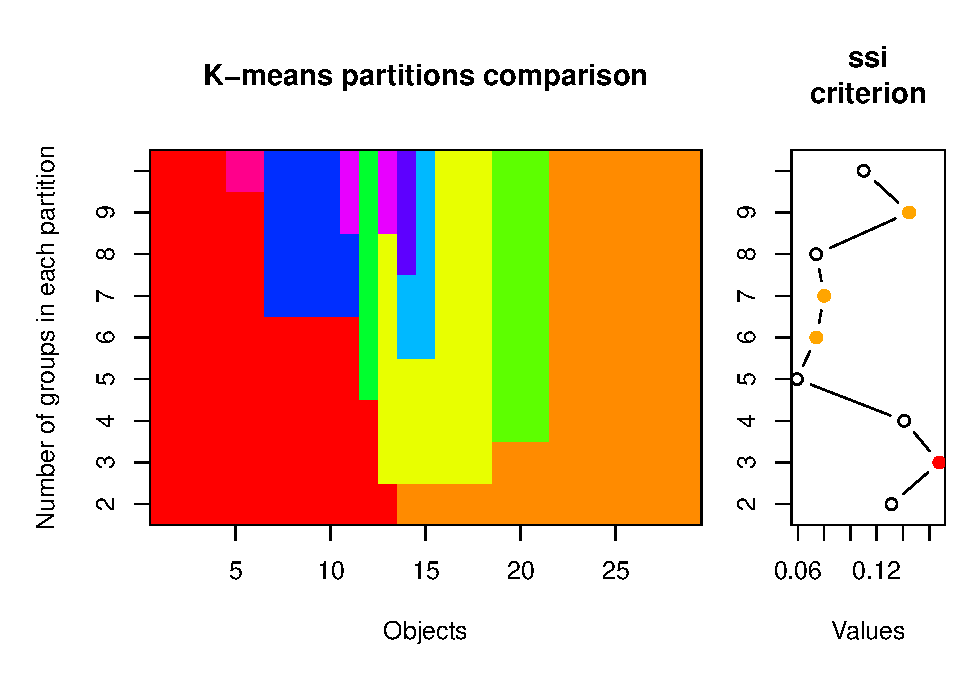
\includegraphics{livro_r_ecologia_files/figure-latex/unnamed-chunk-35-1.pdf}

Este resultado nos mostra que o número ideal de grupos é 3, vejam que o SSI máximo é alcançado neste número de grupos 0.1675852 (também indicado pela bola vermelha no plot).

\#Espécies indicadoras

\hypertarget{backgorund-da-anuxe1lise-2}{%
\section{Backgorund da análise}\label{backgorund-da-anuxe1lise-2}}

Uma pergunta normalmente feita por ecólogos é: qual espécie pode ser indicadora de uma determinada condição ambiental?

O índice IndVal mede dois aspectos das espécies: Especificidade e fidelidade. Uma alta fidelidade significa que espécies ocorrem em todos os locais do grupo e uma alta especificidade significa que as espécies ocorrem somente naquele grupo. Uma boa espécie indicadora é aquela na qual todos os indivíduos ocorrem em todas a amostras referentes a um grupo específico.
A Especificidade é dada pela divisão da abundancia média da espécie no grupo pela somatória das abundancias médias dos grupos. Fidelidade é igual ao número de lugares no grupo onde a espécie está presente dividido pelo número total de lugares do grupo (Dufrêne \& Legendre, 1997).

Espécies raras podem receber o mesmo valor de IndVal das espécies indicadoras e são chamadas de indicadoras assimétricas, i.e., contribuem com a especificidade do habitat mas não servem para predizer grupos. Ao contrário, as espécies indicadoras são verdadeiros indicadores simétricos e podem ser usadas para predizer grupos.

\hypertarget{exemplo-1-2}{%
\section{Exemplo 1:}\label{exemplo-1-2}}

\textbf{Pergunta:}

\begin{quote}
Qual espécie de anfíbio anuro na fase larval pode ser indicadora da fitofisionomia onde é encontrada?
\end{quote}

\textbf{Predições}

\begin{quote}
\begin{itemize}
\tightlist
\item
  1: Espécies terrestres serão indicadoras de área aberta, enquanto espécies arborícolas serão indicadoras de áreas florestais.
\end{itemize}
\end{quote}

\textbf{Variáveis}

\begin{itemize}
\tightlist
\item
  Variáveis resposta

  \begin{itemize}
  \item
    \begin{enumerate}
    \def\labelenumi{\arabic{enumi}.}
    \tightlist
    \item
      Mesma matriz já utilizada contendo a abundância de girinos ao longo de poças na Serra da Bocaina.
    \end{enumerate}
  \end{itemize}
\end{itemize}

\hypertarget{explicauxe7uxe3o-da-anuxe1lise-2}{%
\subsection{Explicação da análise}\label{explicauxe7uxe3o-da-anuxe1lise-2}}

A análise procede da seguinte forma:

\begin{itemize}
\item
  \begin{enumerate}
  \def\labelenumi{\arabic{enumi}.}
  \tightlist
  \item
    Uma matriz de distância é construída e as unidades amostrais são classificadas com alguma análise de agrupamento, hierárquico ou não;
  \end{enumerate}
\item
  \begin{enumerate}
  \def\labelenumi{\arabic{enumi}.}
  \setcounter{enumi}{1}
  \tightlist
  \item
    A variável ambiental para a qual se deseja classificar os grupos é inserida;
  \end{enumerate}
\item
  \begin{enumerate}
  \def\labelenumi{\arabic{enumi}.}
  \setcounter{enumi}{2}
  \tightlist
  \item
    As espécies indicadoreas de cada grupo são formadas através do cálculo da especificidade e fidelidade, obtendo-se o valor de IndVal para cada espécie;
  \end{enumerate}
\item
  \begin{enumerate}
  \def\labelenumi{\arabic{enumi}.}
  \setcounter{enumi}{3}
  \tightlist
  \item
    Por fim, o conjunto de dados originais é comparado para ver se análise faz sentido.
  \end{enumerate}
\end{itemize}

O cálculo da significância do índice de IndVal é feito por aleatorização de Monte Carlo. Assim, o valor do índice é aleatorizado 999 vezes (ou o número de vezes que você optar) dentro dos tratamentos e o valor de \emph{P} é dado pelo número de vezes em que o índice observado foi igual ou maior que os valores aleatorizados.

\hypertarget{anuxe1lise-2}{%
\subsection{Análise}\label{anuxe1lise-2}}

O IndVal está disponível tanto no pacote \texttt{indicspecies} quando no \texttt{labdsv}. Para este exemplo iremos usar o labdsv.

\begin{Shaded}
\begin{Highlighting}[]
\KeywordTok{library}\NormalTok{(labdsv)}
\end{Highlighting}
\end{Shaded}

Primeiro vamos agrupar as unidades amostrais (poças) que informa os grupos de fitofisionomias onde as poças se localizam e para os quais deseja-se encontrar espécies indicadoras:

\begin{Shaded}
\begin{Highlighting}[]
\NormalTok{fitofis <-}\StringTok{ }\KeywordTok{c}\NormalTok{(}\KeywordTok{rep}\NormalTok{(}\DecValTok{1}\NormalTok{,}\DecValTok{4}\NormalTok{), }\KeywordTok{rep}\NormalTok{(}\DecValTok{2}\NormalTok{,}\DecValTok{4}\NormalTok{), }\KeywordTok{rep}\NormalTok{(}\DecValTok{3}\NormalTok{,}\DecValTok{4}\NormalTok{), }\KeywordTok{rep}\NormalTok{(}\DecValTok{4}\NormalTok{,}\DecValTok{4}\NormalTok{), }\KeywordTok{rep}\NormalTok{(}\DecValTok{5}\NormalTok{,}\DecValTok{4}\NormalTok{))}
\end{Highlighting}
\end{Shaded}

\begin{Shaded}
\begin{Highlighting}[]
\NormalTok{resultado <-}\StringTok{ }\KeywordTok{indval}\NormalTok{(bocaina, fitofis)}
\KeywordTok{summary}\NormalTok{(resultado)}\CommentTok{#só exibe o resultado para as espécies indicadoras}
\end{Highlighting}
\end{Shaded}

\begin{verbatim}
##       cluster indicator_value probability
## Rict        1          0.8364       0.014
## Sduar       1          0.7475       0.039
## 
## Sum of probabilities                 =  8.026 
## 
## Sum of Indicator Values              =  7.3 
## 
## Sum of Significant Indicator Values  =  1.58 
## 
## Number of Significant Indicators     =  2 
## 
## Significant Indicator Distribution
## 
## 1 
## 2
\end{verbatim}

Para apresentar uma tabela dos resultados para todas as espécies temos de processar os dados:

\begin{Shaded}
\begin{Highlighting}[]
\NormalTok{resultado}\OperatorTok{$}\NormalTok{maxcls}
\end{Highlighting}
\end{Shaded}

\begin{verbatim}
##    Aper    Bahe    Rict  Cleuco    Dmic    Dmin   Hpoly    Lfur    Pbar    Polf 
##       3       2       1       3       3       1       2       3       1       3 
## Pmelano   Sduar    Shay    Sobt  Ssqual  Bokerm 
##       2       1       3       2       3       2
\end{verbatim}

\begin{Shaded}
\begin{Highlighting}[]
\NormalTok{resultado}\OperatorTok{$}\NormalTok{indcls}
\end{Highlighting}
\end{Shaded}

\begin{verbatim}
##      Aper      Bahe      Rict    Cleuco      Dmic      Dmin     Hpoly      Lfur 
## 0.2432796 0.6487329 0.8363823 0.4128631 0.6645244 0.7032145 0.6208711 0.2279412 
##      Pbar      Polf   Pmelano     Sduar      Shay      Sobt    Ssqual    Bokerm 
## 0.2813725 0.2437500 0.2500000 0.7474527 0.4930269 0.2222222 0.2500000 0.4583333
\end{verbatim}

\begin{Shaded}
\begin{Highlighting}[]
\NormalTok{resultado}\OperatorTok{$}\NormalTok{pval}
\end{Highlighting}
\end{Shaded}

\begin{verbatim}
##    Aper    Bahe    Rict  Cleuco    Dmic    Dmin   Hpoly    Lfur    Pbar    Polf 
##   1.000   0.062   0.014   0.385   0.217   0.086   0.266   1.000   0.615   1.000 
## Pmelano   Sduar    Shay    Sobt  Ssqual  Bokerm 
##   1.000   0.039   0.423   0.698   1.000   0.221
\end{verbatim}

\begin{Shaded}
\begin{Highlighting}[]
\NormalTok{tab.resultado=}\KeywordTok{cbind}\NormalTok{(resultado}\OperatorTok{$}\NormalTok{maxcls,resultado}\OperatorTok{$}\NormalTok{indcls,resultado}\OperatorTok{$}\NormalTok{pval)}
\KeywordTok{colnames}\NormalTok{(tab.resultado)<-}\KeywordTok{c}\NormalTok{(}\StringTok{"maxgrp"}\NormalTok{, }\StringTok{"ind. value"}\NormalTok{,}\StringTok{"P"}\NormalTok{)}
\NormalTok{tab.resultado}
\end{Highlighting}
\end{Shaded}

\begin{verbatim}
##         maxgrp ind. value     P
## Aper         3  0.2432796 1.000
## Bahe         2  0.6487329 0.062
## Rict         1  0.8363823 0.014
## Cleuco       3  0.4128631 0.385
## Dmic         3  0.6645244 0.217
## Dmin         1  0.7032145 0.086
## Hpoly        2  0.6208711 0.266
## Lfur         3  0.2279412 1.000
## Pbar         1  0.2813725 0.615
## Polf         3  0.2437500 1.000
## Pmelano      2  0.2500000 1.000
## Sduar        1  0.7474527 0.039
## Shay         3  0.4930269 0.423
## Sobt         2  0.2222222 0.698
## Ssqual       3  0.2500000 1.000
## Bokerm       2  0.4583333 0.221
\end{verbatim}

No resultado podemos ver que temos duas espécies indicadoras da fitofisionimia 1: \emph{Rhinella icterica} (Rict) e \emph{Scinax duartei} (Sduar). Nenhuma espécie foi indicadora dos outros grupos neste exemplo.

\hypertarget{para-se-aprofundar}{%
\subsection{Para se aprofundar}\label{para-se-aprofundar}}

\begin{itemize}
\tightlist
\item
  \href{https://www.sciencedirect.com/science/article/pii/S0304380010006393?casa_token=0YLFbVbGj1IAAAAA:RFcrLHBDdt-NY5gpxCEAqlc8LMG0ayzChpMvaOFQkE10ftg2Us6PafgMQCSmCZZ21eb430e_lWo}{Agrupamento de espécies e locais baseado em modelos}
\item
  \href{http://adn.biol.umontreal.ca/~numericalecology/numecolR/}{Numerical Ecology with R}
\end{itemize}

\hypertarget{rarefauxe7uxe3o}{%
\chapter{Rarefação}\label{rarefauxe7uxe3o}}

\hypertarget{background-da-anuxe1lise}{%
\section{Background da análise}\label{background-da-anuxe1lise}}

Uma das dificuldades na comparação da riqueza de espécies entre comunidades é decorrente da diferença no esforço amostral (e.g.diferença no número de indivíduos, discrepância na quantidade de unidades amostrais ou área amostrada) que inevitavelmente influenciará no número de espécies observadas (Gotelli \& Chao 2013). O método de rarefação nos permite comparar o número de espécies entre comunidades quando o tamanho da amostra ou a abundância de indivíduos não são iguais. A rarefação calcula o número esperado de espécies em cada comunidade tendo como base comparativa um valor em que todas as amostras atinjam um tamanho padrão, ou comparações baseadas na comunidade com menor número de amostragens ou com menos indivíduos. O teste foi formulado considerando seguinte pergunta: Se considerarmos \emph{n} indivíduos ou amostras (\emph{n} \textless{} N) para cada comunidade, quantas espécies registraríamos nas comunidades considerando o mesmo número de indivíduos ou amostras?

\[E(S) = \sum 1 - \frac{{(N - N_1)}/{n}}{{N}/{n}}\]

Onde:

\begin{itemize}
\item
  E(S) = Número de espécies esperado,
\item
  N = Número total de indivíduos na amostra,
\item
  Ni = Número de indivíduos da iésima espécie,
\item
  \emph{n} = tamanho da amostra padronizada (menor amostra).
\end{itemize}

Gotelli \& Collwel (2001) descrevem este método e discutem em detalhes as restrições sobre seu uso na ecologia:

\begin{itemize}
\tightlist
\item
  As amostras a serem comparados devem ser consistentes do ponto de vista taxonômico, ou seja, todos os indivíduos devem pertencer ao mesmo grupo taxonômico;\\
\item
  As comparações devem ser realizadas somente entre amostras com as mesmas técnicas de coleta;\\
\item
  Os tipos de hábitat onde as amostras são obtidas devem ser semelhantes;\\
\item
  É um método para estimar a riqueza de espécies em uma amostra menor -- não pode ser usado para extrapolar e estimar riqueza.
\end{itemize}

Contudo, é importante ressaltar que esta última restrição foi superada por Colwell et al.~(2012) e Chao \& Jost (2012) que desenvolveram uma nova abordagem onde os dados podem ser interpolados (rarefeito) para amostras menores e extrapolados para amostras maiores.

\hypertarget{exemplo-pruxe1tico-1---morcegos}{%
\section{Exemplo prático 1 - Morcegos}\label{exemplo-pruxe1tico-1---morcegos}}

\hypertarget{explicauxe7uxe3o}{%
\subsection{Explicação}\label{explicauxe7uxe3o}}

\textbf{Explicação dos dados}

Neste exemplo usaremos os dados de espécies de morcegos amostradas em três fragmentos florestais (Breviglieri 2008): i) Mata Ciliar do Córrego Talhadinho com 12 hectares inserida em uma matriz de pastagem; ii) Mata Ciliar do Córrego dos Tenentes com 10 hectares inserida em uma matriz de cultivo de cana-de-açucar e pastagem; e iii) Fazenda Experimental de Pindorama com 128 hectares inserida uma matriz de cana-de-açúcar e pastagem.

\textbf{Pergunta:}

\begin{quote}
A riqueza de espécies de morcegos é maior na Fazenda Experimental do que nos fragmentos florestais menores?
\end{quote}

\textbf{Predições}

\begin{quote}
O número de espécies será maior em fragmentos florestais maiores.
\end{quote}

\textbf{Variáveis}

\begin{itemize}
\tightlist
\item
  Variáveis preditoras

  \begin{itemize}
  \tightlist
  \item
    matriz ou dataframe com as abundâncias das espécies de morcegos registradas nos três fragmentos florestais
  \end{itemize}
\end{itemize}

\textbf{Checklist}

\begin{itemize}
\tightlist
\item
  Verificar se a sua matriz ou dataframe estão com as espécies nas linhas e os fragmentos florestais nas colunas
\end{itemize}

\hypertarget{anuxe1lise}{%
\subsection{Análise}\label{anuxe1lise}}

Calculo da rarefação

\begin{Shaded}
\begin{Highlighting}[]
\KeywordTok{library}\NormalTok{(iNEXT)}
\KeywordTok{library}\NormalTok{(devtools)}
\NormalTok{devtools}\OperatorTok{::}\KeywordTok{install_github}\NormalTok{(}\StringTok{"paternogbc/ecodados"}\NormalTok{)}
\end{Highlighting}
\end{Shaded}

\begin{verbatim}
##   
   checking for file ‘/tmp/Rtmpi56827/remotes4cde443ea656/paternogbc-ecodados-6592f84/DESCRIPTION’ ...
  
v  checking for file ‘/tmp/Rtmpi56827/remotes4cde443ea656/paternogbc-ecodados-6592f84/DESCRIPTION’
## 
  
-  preparing ‘ecodados’:
## 
  
   checking DESCRIPTION meta-information ...
  
v  checking DESCRIPTION meta-information
## 
  
-  checking for LF line-endings in source and make files and shell scripts
## 
  
-  checking for empty or unneeded directories
## -  building ‘ecodados_0.1.0.tar.gz’
## 
  
   
## 
\end{verbatim}

\begin{Shaded}
\begin{Highlighting}[]
\KeywordTok{library}\NormalTok{(ecodados)}

\NormalTok{dados_rarefacao <-}\StringTok{ }\NormalTok{rarefacao_morcegos}
\NormalTok{resultados_morcegos <-}\StringTok{ }\KeywordTok{iNEXT}\NormalTok{(dados_rarefacao, }\DataTypeTok{q =} \DecValTok{0}\NormalTok{, }\DataTypeTok{datatype =} \StringTok{"abundance"}\NormalTok{, }\DataTypeTok{endpoint =} \DecValTok{800}\NormalTok{)}
\CommentTok{# q refere-se a família *Hill-numbers* (Hill 1973) onde 0 = riqueza de espécies, 1 =  diversidade de Shannon, e 2 = diversidade de Simpson.}
\CommentTok{# Veja mais detalhes sobre os números de Hill no Capítulo 7 onde tratamos de extrapolações.}
\CommentTok{# datatype refere-se ao tipo de dados que você vai analisar (e.g. abudância, incidência).}
\CommentTok{# endpoint refere-se ao valor de referência que você determina para a extrapolação.}

\CommentTok{# Visualizar os resultados }
\KeywordTok{ggiNEXT}\NormalTok{(resultados_morcegos, }\DataTypeTok{type =} \DecValTok{1}\NormalTok{)}
\end{Highlighting}
\end{Shaded}

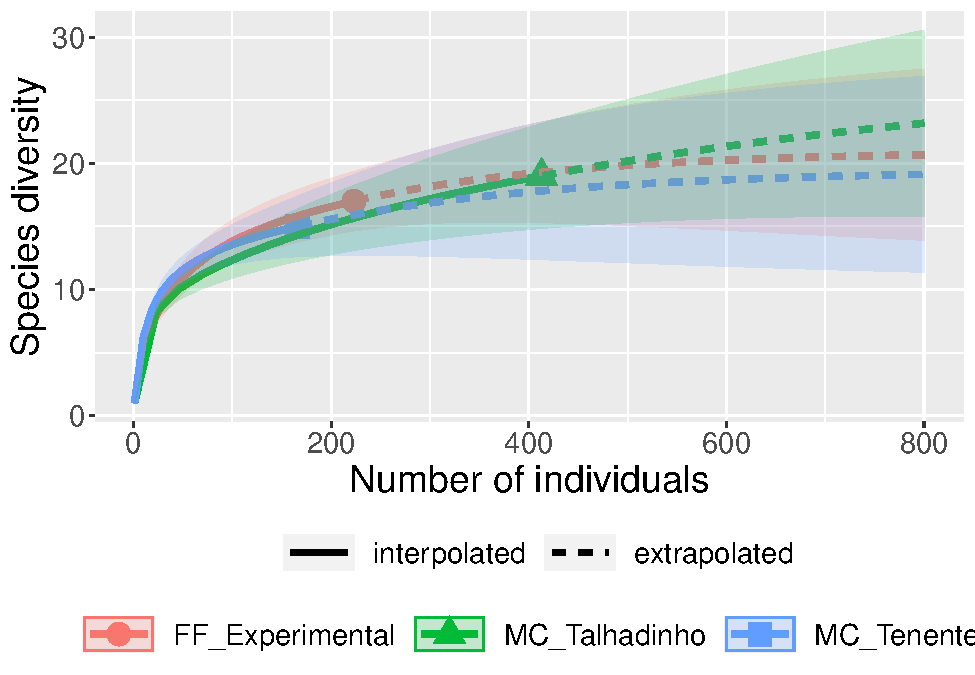
\includegraphics{livro_r_ecologia_files/figure-latex/unnamed-chunk-40-1.pdf}

\hypertarget{interpretauxe7uxe3o-dos-resultados}{%
\subsection{Interpretação dos resultados}\label{interpretauxe7uxe3o-dos-resultados}}

Neste exemplo, foram registrados 166 indivíduos na MC\_Tenentes, 413 na MC\_Talhadinho e 223 na FF\_Experimental. Lembrando, você não pode comparar a riqueza de espécies observada diretamente: 15 espécies na MC\_Tenentes, 17 espécies na MC\_Talhadinho, e 13 espécies no FF\_Experimental. A comparação da riqueza de espécies entre as comunidades deve ser feita com base na riqueza de espécies estimada que é calculada com base no número de indivíduos da comunidade com menor abundância (166 indivíduos). Olhando o gráfico é possível perceber que a riqueza de espécies de morcegos estimada não é diferente entre os três fragmentos florestais quando corrigimos o problema da abundância pela rarefação. A interpretação é feita com base no intervalo de confiança de 95\%. As curvas serão diferentes quando os intervalos de confiança não se sobreporem (Chao et al.~2014). Percebam que está abordagem, além da interpolação (rarefação), também realiza extrapolações que podem ser usadas para estimar o número de espécies caso o esforço de coleta fosse maior. Este é o assunto do nosso próximo capítulo.

~

\hypertarget{exemplo-pruxe1tico-2---rarefauxe7uxe3o}{%
\section{Exemplo prático 2 - Rarefação}\label{exemplo-pruxe1tico-2---rarefauxe7uxe3o}}

\hypertarget{explicauxe7uxe3o-1}{%
\subsection{Explicação}\label{explicauxe7uxe3o-1}}

\textbf{Explicação dos dados}

Neste exemplo iremos comparar o número de espécies de anuros e répteis (serptentes e lagartos) usando informações dos indivíduos depositados em coleções científicas e coletas de campo (da Silva et al.~2017).

\textbf{Pergunta:}

\begin{quote}
A riqueza de espécies de anuros e répteis é maior em coleções científicas do que nas coletas de campo?
\end{quote}

\textbf{Predições}

\begin{quote}
O número de espécies será maior em coleções científicas devido ao maior esforço amostral (i.e.~maior variação temporal para depositar os indíviduos e maior número de pessoas contribuindo com as informações de diferentes estudos e/ou coletas esporádicas).
\end{quote}

\textbf{Variáveis}

\begin{itemize}
\tightlist
\item
  Variáveis preditoras

  \begin{itemize}
  \tightlist
  \item
    matriz ou dataframe com as abundâncias das espécies de anuros e répteis (planilhas separadas) registradas em coleções científicas e coletas de campo.
  \end{itemize}
\end{itemize}

\textbf{Checklist}

\begin{itemize}
\tightlist
\item
  Verificar se a sua matriz ou dataframe estão com as espécies nas linhas e a fonte dos dados nas colunas.
\end{itemize}

\hypertarget{anuxe1lise-1}{%
\subsection{Análise}\label{anuxe1lise-1}}

Calculo da rarefação para os dados de répteis

\begin{Shaded}
\begin{Highlighting}[]
\KeywordTok{library}\NormalTok{(iNEXT)}

\NormalTok{rarefacao_repteis <-}\StringTok{ }\NormalTok{rarefacao_repteis}
\NormalTok{resultados_repteis <-}\StringTok{ }\KeywordTok{iNEXT}\NormalTok{(rarefacao_repteis, }\DataTypeTok{q =} \DecValTok{0}\NormalTok{, }\DataTypeTok{datatype =} \StringTok{"abundance"}\NormalTok{, }\DataTypeTok{endpoint =} \DecValTok{200}\NormalTok{)}

\CommentTok{# Visualizar os resultados }
\KeywordTok{ggiNEXT}\NormalTok{(resultados_repteis, }\DataTypeTok{type =} \DecValTok{1}\NormalTok{)}
\end{Highlighting}
\end{Shaded}

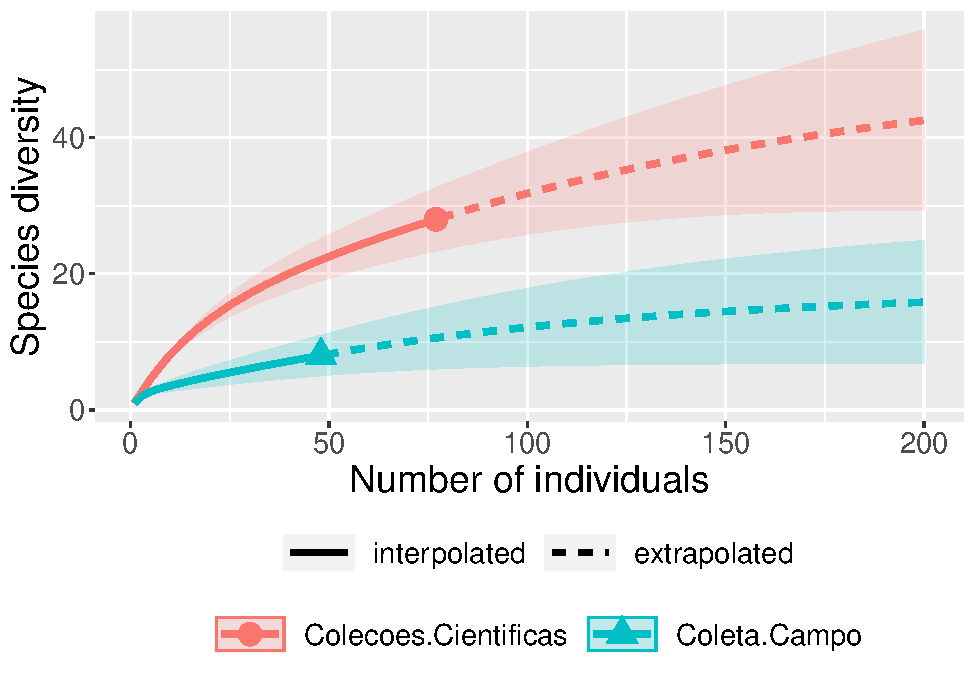
\includegraphics{livro_r_ecologia_files/figure-latex/unnamed-chunk-41-1.pdf}

\hypertarget{interpretauxe7uxe3o-dos-resultados-1}{%
\subsection{Interpretação dos resultados}\label{interpretauxe7uxe3o-dos-resultados-1}}

Neste exemplo,foram registradas oito espécies de répteis nas coletas de campo (40 indivíduos) e 28 espécies nas coleções científicas (77 indivíduos). Com base na rarefação, concluímos que a riqueza de espécies de répteis obtida nas coleções científicas é 2,5 vezes maior do que a obtida em coletas de campo.

~

Calculo da rarefação para os dados dos anuros

\begin{Shaded}
\begin{Highlighting}[]
\KeywordTok{library}\NormalTok{(iNEXT)}

\NormalTok{rarefacao_anuros <-}\StringTok{ }\NormalTok{rarefacao_anuros}
\NormalTok{resultados_anuros <-}\StringTok{ }\KeywordTok{iNEXT}\NormalTok{(rarefacao_anuros, }\DataTypeTok{q =} \DecValTok{0}\NormalTok{, }\DataTypeTok{datatype =} \StringTok{"abundance"}\NormalTok{, }\DataTypeTok{endpoint =} \DecValTok{800}\NormalTok{)}

\CommentTok{# Visualizar os resultados }
\KeywordTok{ggiNEXT}\NormalTok{(resultados_anuros, }\DataTypeTok{type =} \DecValTok{1}\NormalTok{, }\DataTypeTok{grey =} \OtherTok{TRUE}\NormalTok{)}
\end{Highlighting}
\end{Shaded}

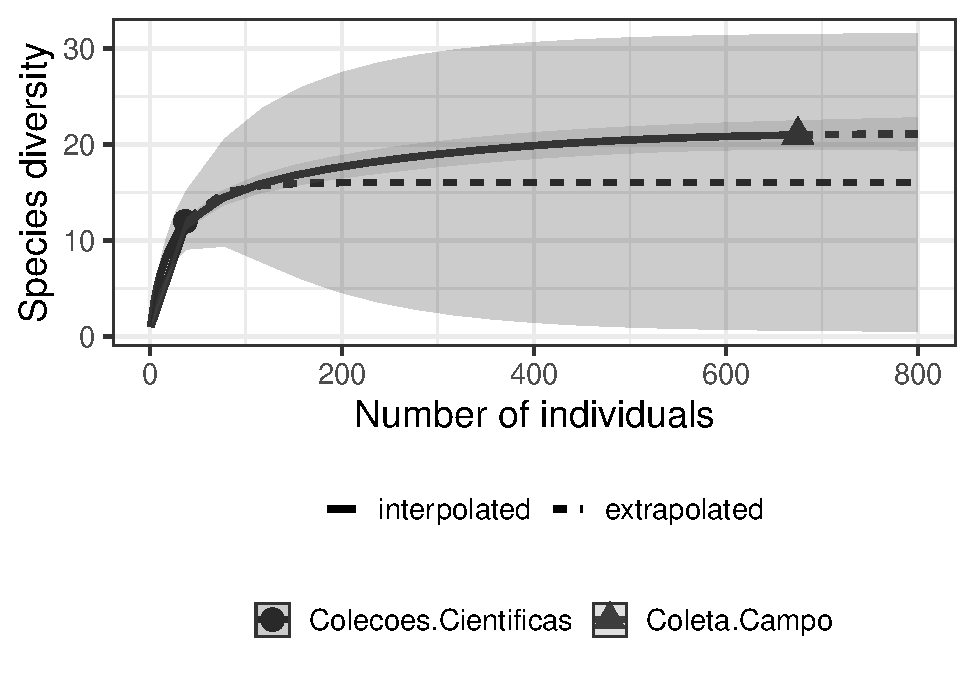
\includegraphics{livro_r_ecologia_files/figure-latex/unnamed-chunk-42-1.pdf}

\textbf{Interpretação dos resultados}

Neste exemplo,foram registradas 21 espécies de anuros nas coletas de campo (709 indivíduos) e 12 espécies nas coleções científicas (37 indivíduos). Com base na rarefação, concluímos que não há diferença entre a riqueza de espécies de anuros obtida em coletas de campo e coleções científicas.

~

\hypertarget{para-se-aprofundar}{%
\section{Para se aprofundar}\label{para-se-aprofundar}}

\begin{itemize}
\item
  Recomendamos aos interessados que olhem a página do \href{http://viceroy.eeb.uconn.edu/estimates}{EstimateS software} e baixem o manual do usuário que contém informações detalhadas sobre os índices de rarefação.Este site foi criado e é mantido pelo Dr.~Robert K. Colwell, um dos maiores especialistas do mundo em estimativas da biodiversidade
\item
  Recomendamos também o livro Magurran \& McGill (2010) - Biological Diversity Frontiers in Measurement and Assessment.
\end{itemize}

\hypertarget{estimadores-de-riqueza}{%
\chapter{Estimadores de Riqueza}\label{estimadores-de-riqueza}}

\hypertarget{backgorund-da-anuxe1lise}{%
\section{Backgorund da análise}\label{backgorund-da-anuxe1lise}}

Uma vez que determinar o número total de espécies numa área é praticamente impossível, principalmente em regiões com alta riqueza de espécies, os estimadores são úteis para extrapolar a riqueza observada e tentar estimar a riqueza total através de uma amostra incompleta de uma comunidade biológica (Walther \& Moore 2005). Neste capítulo serão considerados os estimadores não paramétricos que usam informações da frequencia de espécies raras na comunidade (Gotelli \& Chao 2013). Isto porque tanto os testes paramétricos que tentam determinar os parâmetros de uma curva usando o formato da curva de acumulação de espécies (e.g.~equação logística, Michaelis-Menten) quanto os testes que usam a frequencia do número de indivíduos para enquadrá-las em uma das distribuições de abundância das espécies (e.g.~distribuições log-séries, log-normal) não funcionam muito bem com dados empíricos (Gotelli \& Chao 2013). Para mais detalhes sobre os testes paramétricos veja Magurran (2004) e Colwell (2019).

\begin{quote}
\hypertarget{quatro-caracteruxedsticas-para-um-bom-estimador-de-riqueza-chazdon-et-al.-1998-horter-et-al.-2006}{%
\subsubsection{Quatro características para um bom estimador de riqueza (Chazdon et al.~1998; Horter et al.~2006):}\label{quatro-caracteruxedsticas-para-um-bom-estimador-de-riqueza-chazdon-et-al.-1998-horter-et-al.-2006}}

\begin{itemize}
\tightlist
\item
  Independência do tamanho da amostra (quantidade de esforço amostral realizado);
\item
  Insensibilidade a diferentes padrões de distribuições (diferentes equitabilidades);
\item
  Insensibilidade em relação à ordem das amostragens;
\item
  Insensibilidade à heterogeneidade entre as amostras usadas entre estudos.
\end{itemize}
\end{quote}

\hypertarget{estimadores-baseados-na-abunduxe2ncia-das-espuxe9cies}{%
\section{Estimadores baseados na abundância das espécies}\label{estimadores-baseados-na-abunduxe2ncia-das-espuxe9cies}}

\hypertarget{chao-1---chao-1984-1987}{%
\subsection{CHAO 1 - (Chao 1984, 1987):}\label{chao-1---chao-1984-1987}}

Estimador simples do número absoluto de espécies em uma comunidade. É baseado no número de espécies raras dentro de uma amostra.

\begin{quote}
\[Chao_{1} = S_{obs} + \left(\frac{n-1}{n}\right)\frac{F_1(F_1-1)}{2(F_2+1)}\]
\end{quote}

onde:

\begin{itemize}
\item
  Sobs = o número de espécies na comunidade,
\item
  \emph{n} = número de amostras,
\item
  F1 = número de espécies observadas com abundância de um indivíduo (espécies \emph{singleton}),
\item
  F2 = número de espécies observadas com abundância de dois indivíduos (espécies \emph{doubletons}).
\end{itemize}

O valor de Chao 1 é máximo quando todas as espécies menos uma são únicas (\emph{singleton}). Neste caso, a riqueza estimada é aproximadamente o dobro da riqueza observada.

~

\hypertarget{exemplo-pruxe1tico---chao-1}{%
\subsubsection{Exemplo prático - Chao 1}\label{exemplo-pruxe1tico---chao-1}}

\hypertarget{explicauxe7uxe3o-dos-dados}{%
\paragraph{Explicação dos dados}\label{explicauxe7uxe3o-dos-dados}}

Neste exemplo usaremos os dados de 17 espécies de anuros amostradas em 14 dias de coletas de campo em um habitat reprodutivo localizado na região noroeste do estado de São Paulo, Brasil.

\textbf{Pergunta:}

\begin{quote}
Quantas espécies a mais poderiam ser amostradas caso aumentassemos o esforço amostral?
\end{quote}

\textbf{Predições}

\begin{quote}
\begin{itemize}
\tightlist
\item
  O número de espécies estimadas é similar ao número de espécies observada;
\item
  O número de espécies estimadas é maior do que o número de espécies observada.
\end{itemize}
\end{quote}

\textbf{Variáveis}

\begin{itemize}
\tightlist
\item
  Variáveis preditoras

  \begin{itemize}
  \tightlist
  \item
    matriz ou vetor com as abundâncias das espécies de anuros registradas em um habitat reprodutivo
  \end{itemize}
\end{itemize}

\textbf{Checklist}

\begin{itemize}
\tightlist
\item
  Verificar se a sua matriz está com as espécies nas colunas e as amostragens nas linhas
\item
  Verificar se os dados são de abundância e não presença e ausência
\end{itemize}

\hypertarget{anuxe1lise}{%
\subsection{Análise}\label{anuxe1lise}}

Calculo do estimador de riqueza - Chao 1

\begin{Shaded}
\begin{Highlighting}[]
\KeywordTok{library}\NormalTok{(ecodados)}
\KeywordTok{library}\NormalTok{(vegan)}
\NormalTok{dados_coleta <-}\StringTok{ }\NormalTok{poca_anuros}
\NormalTok{est_chao1 <-}\StringTok{ }\KeywordTok{estaccumR}\NormalTok{(dados_coleta, }\DataTypeTok{permutations =} \DecValTok{100}\NormalTok{)}
\KeywordTok{summary}\NormalTok{(est_chao1, }\DataTypeTok{display =} \StringTok{"chao"}\NormalTok{)}
\end{Highlighting}
\end{Shaded}

\begin{verbatim}
## $chao
##         N      Chao   2.5%    97.5%  Std.Dev
## Dia_14  1  7.050833  3.000 12.33333 2.670055
## Dia_5   2 10.135714  6.000 18.81250 3.178221
## Dia_9   3 11.843167  8.000 18.00000 2.637843
## Dia_4   4 12.489167  8.475 17.00000 2.473219
## Dia_11  5 13.386667  9.000 20.00000 2.901766
## Dia_13  6 14.106667  9.475 22.00000 2.925709
## Dia_3   7 14.760000 10.475 22.00000 2.956030
## Dia_10  8 15.716667 11.000 22.00000 3.054270
## Dia_1   9 16.488333 11.475 22.00000 3.031286
## Dia_7  10 17.560000 13.000 22.00000 2.939869
## Dia_8  11 18.320000 13.000 22.00000 2.580541
## Dia_12 12 19.065000 14.000 22.00000 2.164515
## Dia_2  13 19.655000 15.500 22.00000 1.362735
## Dia_6  14 20.000000 20.000 20.00000 0.000000
## 
## attr(,"class")
## [1] "summary.poolaccum"
\end{verbatim}

Visualizar os resultados com intervalo de confiança de 95\%.

\begin{Shaded}
\begin{Highlighting}[]
\KeywordTok{library}\NormalTok{(ggplot2)}
\CommentTok{# preparando os dados para fazer o gráfico}
\NormalTok{resultados <-}\StringTok{ }\KeywordTok{summary}\NormalTok{(est_chao1, }\DataTypeTok{display =} \KeywordTok{c}\NormalTok{(}\StringTok{"S"}\NormalTok{, }\StringTok{"chao"}\NormalTok{))}
\NormalTok{res_chao <-}\StringTok{ }\KeywordTok{cbind}\NormalTok{(resultados}\OperatorTok{$}\NormalTok{chao[,}\DecValTok{1}\OperatorTok{:}\DecValTok{4}\NormalTok{], resultados}\OperatorTok{$}\NormalTok{S[,}\DecValTok{2}\OperatorTok{:}\DecValTok{4}\NormalTok{])}
\NormalTok{res_chao <-}\StringTok{ }\KeywordTok{as.data.frame}\NormalTok{(res_chao)}
\KeywordTok{colnames}\NormalTok{(res_chao) <-}\StringTok{ }\KeywordTok{c}\NormalTok{(}\StringTok{"Amostras"}\NormalTok{, }\StringTok{"Chao"}\NormalTok{, }\StringTok{"C_inferior"}\NormalTok{, }\StringTok{"C_superior"}\NormalTok{, }\StringTok{"Riqueza"}\NormalTok{,}
                        \StringTok{"R_inferior"}\NormalTok{, }\StringTok{"R_superior"}\NormalTok{)}

\CommentTok{# comando para o gráfico}
\KeywordTok{ggplot}\NormalTok{(res_chao, }\KeywordTok{aes}\NormalTok{(}\DataTypeTok{y =}\NormalTok{ Riqueza, }\DataTypeTok{x =}\NormalTok{ Amostras)) }\OperatorTok{+}
\StringTok{  }\KeywordTok{geom_point}\NormalTok{(}\KeywordTok{aes}\NormalTok{(}\DataTypeTok{y =}\NormalTok{ Chao, }\DataTypeTok{x =}\NormalTok{ Amostras }\OperatorTok{+}\StringTok{ }\FloatTok{0.1}\NormalTok{), }\DataTypeTok{size =} \DecValTok{5}\NormalTok{, }\DataTypeTok{color =} \StringTok{"blue"}\NormalTok{, }\DataTypeTok{alpha =} \DecValTok{1}\NormalTok{) }\OperatorTok{+}
\StringTok{  }\KeywordTok{geom_point}\NormalTok{(}\KeywordTok{aes}\NormalTok{(}\DataTypeTok{y =}\NormalTok{ Riqueza, }\DataTypeTok{x =}\NormalTok{ Amostras), }\DataTypeTok{size =} \DecValTok{5}\NormalTok{, }\DataTypeTok{color =} \StringTok{"red"}\NormalTok{, }\DataTypeTok{alpha =} \DecValTok{1}\NormalTok{) }\OperatorTok{+}
\StringTok{  }\KeywordTok{geom_line}\NormalTok{ (}\KeywordTok{aes}\NormalTok{(}\DataTypeTok{y =}\NormalTok{ Chao, }\DataTypeTok{x =}\NormalTok{ Amostras), }\DataTypeTok{color =} \StringTok{"blue"}\NormalTok{) }\OperatorTok{+}
\StringTok{  }\KeywordTok{geom_line}\NormalTok{ (}\KeywordTok{aes}\NormalTok{(}\DataTypeTok{y =}\NormalTok{ Riqueza, }\DataTypeTok{x =}\NormalTok{ Amostras), }\DataTypeTok{color =} \StringTok{"red"}\NormalTok{) }\OperatorTok{+}
\StringTok{  }\KeywordTok{geom_linerange}\NormalTok{(}\KeywordTok{aes}\NormalTok{(}\DataTypeTok{ymin =}\NormalTok{ C_inferior, }\DataTypeTok{ymax =}\NormalTok{ C_superior, }\DataTypeTok{x =}\NormalTok{ Amostras }\OperatorTok{+}\StringTok{ }\FloatTok{0.1}\NormalTok{),}
 \DataTypeTok{color =} \StringTok{"blue"}\NormalTok{) }\OperatorTok{+}
\StringTok{  }\KeywordTok{geom_linerange}\NormalTok{(}\KeywordTok{aes}\NormalTok{(}\DataTypeTok{ymin =}\NormalTok{ R_inferior, }\DataTypeTok{ymax =}\NormalTok{ R_superior, }\DataTypeTok{x =}\NormalTok{ Amostras), }\DataTypeTok{color =} \StringTok{"red"}\NormalTok{) }\OperatorTok{+}
\StringTok{  }\KeywordTok{ylab}\NormalTok{ (}\StringTok{"Estimador de riqueza - Chao 1"}\NormalTok{) }\OperatorTok{+}
\StringTok{  }\KeywordTok{xlab}\NormalTok{ (}\StringTok{"Número de amostras"}\NormalTok{) }\OperatorTok{+}
\StringTok{  }\KeywordTok{scale_x_continuous}\NormalTok{(}\DataTypeTok{limits =} \KeywordTok{c}\NormalTok{(}\DecValTok{1}\NormalTok{,}\DecValTok{15}\NormalTok{), }\DataTypeTok{breaks=}\KeywordTok{seq}\NormalTok{(}\DecValTok{1}\NormalTok{,}\DecValTok{15}\NormalTok{,}\DecValTok{1}\NormalTok{)) }\OperatorTok{+}
\StringTok{  }\KeywordTok{geom_point}\NormalTok{(}\DataTypeTok{y=} \FloatTok{7.5}\NormalTok{, }\DataTypeTok{x =} \DecValTok{9}\NormalTok{, }\DataTypeTok{size =} \DecValTok{5}\NormalTok{, }\DataTypeTok{color =} \StringTok{"blue"}\NormalTok{, }\DataTypeTok{alpha =} \DecValTok{1}\NormalTok{) }\OperatorTok{+}\StringTok{ }
\StringTok{  }\KeywordTok{geom_point}\NormalTok{(}\DataTypeTok{y=} \FloatTok{5.9}\NormalTok{, }\DataTypeTok{x =} \DecValTok{9}\NormalTok{, }\DataTypeTok{size =} \DecValTok{5}\NormalTok{, }\DataTypeTok{color =} \StringTok{"red"}\NormalTok{, }\DataTypeTok{alpha =} \DecValTok{1}\NormalTok{) }\OperatorTok{+}\StringTok{ }
\StringTok{  }\KeywordTok{geom_label}\NormalTok{( }\DataTypeTok{y =} \FloatTok{7.5}\NormalTok{, }\DataTypeTok{x =} \DecValTok{12}\NormalTok{, }\DataTypeTok{label =} \StringTok{"Riqueza estimada - Chao 1"}\NormalTok{) }\OperatorTok{+}
\StringTok{  }\KeywordTok{geom_label}\NormalTok{( }\DataTypeTok{y =} \FloatTok{5.9}\NormalTok{, }\DataTypeTok{x =} \FloatTok{11.3}\NormalTok{, }\DataTypeTok{label =} \StringTok{"Riqueza observada"}\NormalTok{)}
\end{Highlighting}
\end{Shaded}

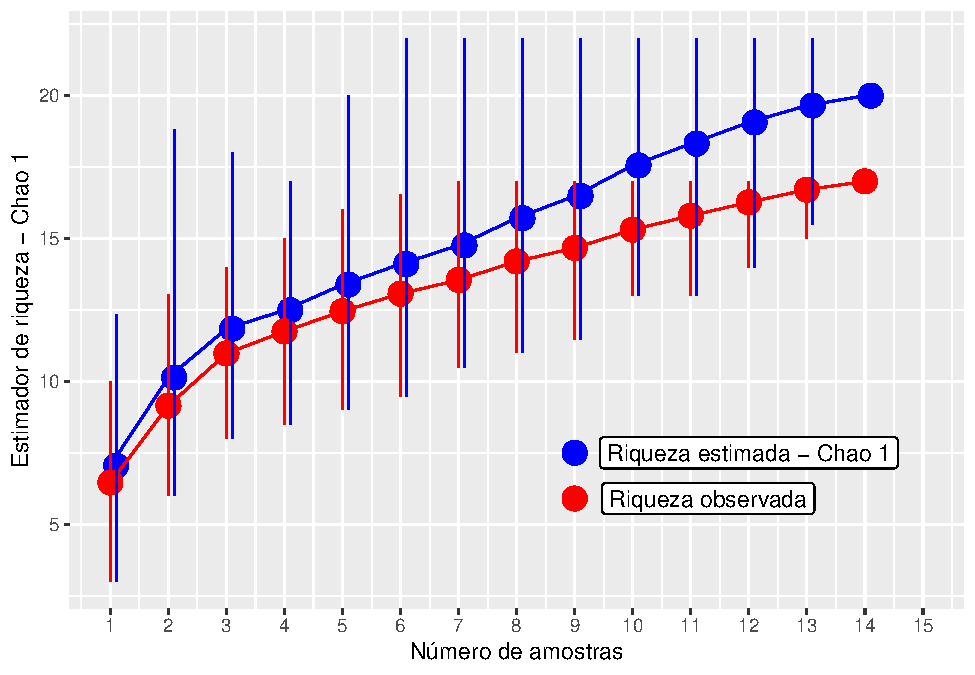
\includegraphics{livro_r_ecologia_files/figure-latex/unnamed-chunk-44-1.pdf}

\hypertarget{interpretauxe7uxe3o-dos-resultados}{%
\subsubsection{Interpretação dos resultados}\label{interpretauxe7uxe3o-dos-resultados}}

Com base no número de espécies raras (\emph{singletons} e \emph{doubletons}), o estimador Chao 1 indica a possibilidade de encontrarmos mais três espécies caso o esforço amostral fosse maior e não mostra tendência de estabilização da curva em uma assíntota.

\hypertarget{ace---abundance-based-coverage-estimador-chao-lee-1992-chao-et-al.-2000}{%
\subsection{\texorpdfstring{ACE - \emph{Abundance-based Coverage Estimador} (Chao \& Lee 1992, Chao et al.~2000):}{ACE - Abundance-based Coverage Estimador (Chao \& Lee 1992, Chao et al.~2000):}}\label{ace---abundance-based-coverage-estimador-chao-lee-1992-chao-et-al.-2000}}

Este método trabalha com a abundância das espécies raras (i.e.~abundância baixa). Entretanto, diferente do estimador anterior, esse método permite ao pesquisador determinar os limites para os quais uma espécie seja considerada rara. Em geral, são consideradas raras espécies com abundância entre 1 e 10 indivíduos. A riqueza estimada pode variar conforme se aumente ou diminua o limiar de abundância, e infelizmente não existem critérios biológicos definidos para a escolha do melhor intervalo.

\begin{quote}
\[ACE = S_{abund} + \frac{S_{rare}}{C_{ace}} + \frac{F_1}{C_{ace}}Y_{ace}^2\]
\end{quote}

onde:

\begin{quote}
\[Y_{ace}^2 = max \left[\frac{S_{rare}}{C_{ace}}\frac{\sum_{i=i}^{10}i(i-1)F1}{(N_{rare})({N_{rare} - 1)}}-1,0\right]\]
\end{quote}

\begin{quote}
\[C_{ace} = 1 - \frac{F1}{N_{rare}}\]
\end{quote}

\begin{quote}
\[N_{rare} = \sum_{i=1}^{10}iF_i\]
\end{quote}

Não precisa fazer cara feia, é óbvio que iremos usar o programa para fazer esses cálculos.

~

\hypertarget{exemplo-pruxe1tico---ace}{%
\subsubsection{Exemplo prático - ACE}\label{exemplo-pruxe1tico---ace}}

\hypertarget{explicauxe7uxe3o-dos-dados-1}{%
\paragraph{Explicação dos dados}\label{explicauxe7uxe3o-dos-dados-1}}

Usaremos os mesmos dados de 17 espécies de anuros amostradas em 14 dias de coletas de campo em um habitat reprodutivo localizado na região noroeste do estado de São Paulo, Brasil.

\textbf{Pergunta:}

\begin{quote}
Quantas espécies a mais poderiam ser amostradas caso aumentassemos o esforço amostral?
\end{quote}

\textbf{Predições}

\begin{quote}
\begin{itemize}
\tightlist
\item
  O número de espécies estimadas é similar ao número de espécies observada;
\item
  O número de espécies estimadas é maior do que o número de espécies observada.
\end{itemize}
\end{quote}

\textbf{Variáveis}

\begin{itemize}
\tightlist
\item
  Variáveis preditoras

  \begin{itemize}
  \tightlist
  \item
    matriz ou vetor com as abundâncias das espécies de anuros registradas em um habitat reprodutivo
  \end{itemize}
\end{itemize}

\textbf{Checklist}

\begin{itemize}
\tightlist
\item
  Verificar se a sua matriz está com as espécies nas colunas e as amostragens nas linhas
\item
  Verificar se os dados são de abundância e não presença e ausência
\end{itemize}

\hypertarget{anuxe1lise-1}{%
\subsection{Análise}\label{anuxe1lise-1}}

Calculo do estimador de riqueza - ACE

\begin{Shaded}
\begin{Highlighting}[]
\KeywordTok{library}\NormalTok{(vegan)}
\NormalTok{dados_coleta <-}\StringTok{ }\NormalTok{poca_anuros}
\NormalTok{est_ace <-}\StringTok{ }\KeywordTok{estaccumR}\NormalTok{(dados_coleta, }\DataTypeTok{permutations =} \DecValTok{100}\NormalTok{)}
\KeywordTok{summary}\NormalTok{(est_ace, }\DataTypeTok{display =} \StringTok{"ace"}\NormalTok{)}
\end{Highlighting}
\end{Shaded}

\begin{verbatim}
## $ace
##         N       ACE      2.5%    97.5%  Std.Dev
## Dia_4   1  7.233102  3.545190 13.71429 2.787760
## Dia_5   2  9.949211  6.000000 18.43698 3.089797
## Dia_3   3 11.082845  6.475000 17.22038 2.751973
## Dia_9   4 12.316111  8.000000 18.28983 2.501741
## Dia_6   5 13.606292  9.112879 19.53118 2.438057
## Dia_12  6 14.599382 10.000000 21.25001 2.829922
## Dia_13  7 15.506053 11.000000 20.93667 2.719453
## Dia_7   8 16.885254 11.475000 22.76955 3.132128
## Dia_11  9 18.137683 12.430045 24.93470 3.401309
## Dia_1  10 20.020101 13.482634 25.72368 4.027058
## Dia_14 11 21.745625 13.688329 25.72368 3.737003
## Dia_2  12 23.407233 16.904925 25.72368 2.850822
## Dia_10 13 24.563953 19.250000 25.72368 1.511508
## Dia_8  14 24.703704 24.703704 24.70370 0.000000
## 
## attr(,"class")
## [1] "summary.poolaccum"
\end{verbatim}

Visualizar os resultados com intervalo de confiança de 95\%

\begin{Shaded}
\begin{Highlighting}[]
\KeywordTok{library}\NormalTok{(ggplot2)}
\CommentTok{# preparando os dados para fazer o gráfico}
\NormalTok{resultados_ace <-}\StringTok{ }\KeywordTok{summary}\NormalTok{(est_ace, }\DataTypeTok{display =} \KeywordTok{c}\NormalTok{(}\StringTok{"S"}\NormalTok{, }\StringTok{"ace"}\NormalTok{))}
\NormalTok{res_ace <-}\StringTok{ }\KeywordTok{cbind}\NormalTok{(resultados_ace}\OperatorTok{$}\NormalTok{ace[,}\DecValTok{1}\OperatorTok{:}\DecValTok{4}\NormalTok{], resultados_ace}\OperatorTok{$}\NormalTok{S[,}\DecValTok{2}\OperatorTok{:}\DecValTok{4}\NormalTok{])}
\NormalTok{res_ace <-}\StringTok{ }\KeywordTok{as.data.frame}\NormalTok{(res_ace)}
\KeywordTok{colnames}\NormalTok{(res_ace) <-}\StringTok{ }\KeywordTok{c}\NormalTok{(}\StringTok{"Amostras"}\NormalTok{, }\StringTok{"ACE"}\NormalTok{, }\StringTok{"ACE_inferior"}\NormalTok{, }\StringTok{"ACE_superior"}\NormalTok{, }\StringTok{"Riqueza"}\NormalTok{,}
                        \StringTok{"R_inferior"}\NormalTok{, }\StringTok{"R_superior"}\NormalTok{)}

\CommentTok{# comando para o gráfico}
\KeywordTok{ggplot}\NormalTok{(res_ace, }\KeywordTok{aes}\NormalTok{(}\DataTypeTok{y =}\NormalTok{ Riqueza, }\DataTypeTok{x =}\NormalTok{ Amostras)) }\OperatorTok{+}
\StringTok{  }\KeywordTok{geom_point}\NormalTok{(}\KeywordTok{aes}\NormalTok{(}\DataTypeTok{y =}\NormalTok{ ACE, }\DataTypeTok{x =}\NormalTok{ Amostras }\OperatorTok{+}\StringTok{ }\FloatTok{0.1}\NormalTok{), }\DataTypeTok{size =} \DecValTok{5}\NormalTok{, }\DataTypeTok{color =} \StringTok{"blue"}\NormalTok{, }\DataTypeTok{alpha =} \DecValTok{1}\NormalTok{) }\OperatorTok{+}
\StringTok{  }\KeywordTok{geom_point}\NormalTok{(}\KeywordTok{aes}\NormalTok{(}\DataTypeTok{y =}\NormalTok{ Riqueza, }\DataTypeTok{x =}\NormalTok{ Amostras), }\DataTypeTok{size =} \DecValTok{5}\NormalTok{, }\DataTypeTok{color =} \StringTok{"red"}\NormalTok{, }\DataTypeTok{alpha =} \DecValTok{1}\NormalTok{) }\OperatorTok{+}
\StringTok{  }\KeywordTok{geom_line}\NormalTok{ (}\KeywordTok{aes}\NormalTok{(}\DataTypeTok{y =}\NormalTok{ ACE, }\DataTypeTok{x =}\NormalTok{ Amostras), }\DataTypeTok{color =} \StringTok{"blue"}\NormalTok{) }\OperatorTok{+}
\StringTok{  }\KeywordTok{geom_line}\NormalTok{ (}\KeywordTok{aes}\NormalTok{(}\DataTypeTok{y =}\NormalTok{ Riqueza, }\DataTypeTok{x =}\NormalTok{ Amostras), }\DataTypeTok{color =} \StringTok{"red"}\NormalTok{) }\OperatorTok{+}
\StringTok{  }\KeywordTok{geom_linerange}\NormalTok{(}\KeywordTok{aes}\NormalTok{(}\DataTypeTok{ymin =}\NormalTok{ ACE_inferior, }\DataTypeTok{ymax =}\NormalTok{ ACE_superior, }\DataTypeTok{x =}\NormalTok{ Amostras }\OperatorTok{+}\StringTok{ }\FloatTok{0.1}\NormalTok{),}
 \DataTypeTok{color =} \StringTok{"blue"}\NormalTok{) }\OperatorTok{+}
\StringTok{  }\KeywordTok{geom_linerange}\NormalTok{(}\KeywordTok{aes}\NormalTok{(}\DataTypeTok{ymin =}\NormalTok{ R_inferior, }\DataTypeTok{ymax =}\NormalTok{ R_superior, }\DataTypeTok{x =}\NormalTok{ Amostras), }\DataTypeTok{color =} \StringTok{"red"}\NormalTok{) }\OperatorTok{+}
\StringTok{  }\KeywordTok{ylab}\NormalTok{ (}\StringTok{"Estimador de riqueza - ACE"}\NormalTok{) }\OperatorTok{+}
\StringTok{  }\KeywordTok{xlab}\NormalTok{ (}\StringTok{"Número de amostras"}\NormalTok{) }\OperatorTok{+}
\StringTok{  }\KeywordTok{scale_x_continuous}\NormalTok{(}\DataTypeTok{limits =} \KeywordTok{c}\NormalTok{(}\DecValTok{1}\NormalTok{,}\DecValTok{15}\NormalTok{), }\DataTypeTok{breaks=}\KeywordTok{seq}\NormalTok{(}\DecValTok{1}\NormalTok{,}\DecValTok{15}\NormalTok{,}\DecValTok{1}\NormalTok{)) }\OperatorTok{+}
\StringTok{  }\KeywordTok{geom_point}\NormalTok{(}\DataTypeTok{y=} \FloatTok{7.5}\NormalTok{, }\DataTypeTok{x =} \DecValTok{9}\NormalTok{, }\DataTypeTok{size =} \DecValTok{5}\NormalTok{, }\DataTypeTok{color =} \StringTok{"blue"}\NormalTok{, }\DataTypeTok{alpha =} \DecValTok{1}\NormalTok{) }\OperatorTok{+}\StringTok{ }
\StringTok{  }\KeywordTok{geom_point}\NormalTok{(}\DataTypeTok{y=} \FloatTok{5.9}\NormalTok{, }\DataTypeTok{x =} \DecValTok{9}\NormalTok{, }\DataTypeTok{size =} \DecValTok{5}\NormalTok{, }\DataTypeTok{color =} \StringTok{"red"}\NormalTok{, }\DataTypeTok{alpha =} \DecValTok{1}\NormalTok{) }\OperatorTok{+}\StringTok{ }
\StringTok{  }\KeywordTok{geom_label}\NormalTok{( }\DataTypeTok{y =} \FloatTok{7.5}\NormalTok{, }\DataTypeTok{x =} \FloatTok{11.7}\NormalTok{, }\DataTypeTok{label =} \StringTok{"Riqueza estimada - ACE"}\NormalTok{) }\OperatorTok{+}
\StringTok{  }\KeywordTok{geom_label}\NormalTok{( }\DataTypeTok{y =} \FloatTok{5.9}\NormalTok{, }\DataTypeTok{x =} \FloatTok{11.3}\NormalTok{, }\DataTypeTok{label =} \StringTok{"Riqueza observada"}\NormalTok{)}
\end{Highlighting}
\end{Shaded}

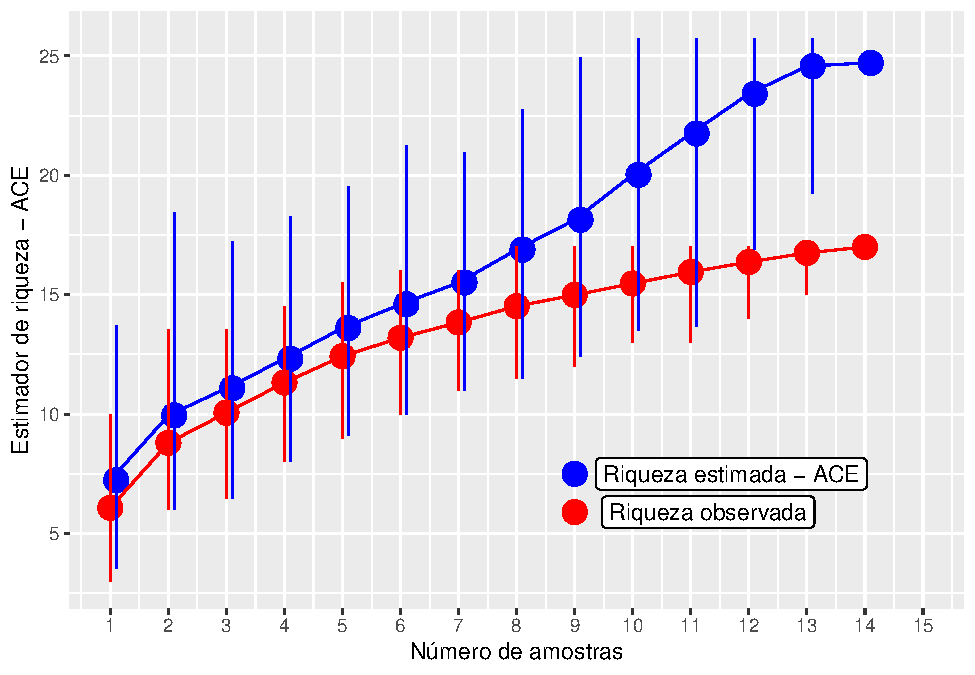
\includegraphics{livro_r_ecologia_files/figure-latex/unnamed-chunk-46-1.pdf}

\hypertarget{interpretauxe7uxe3o-dos-resultados-1}{%
\subsubsection{Interpretação dos resultados}\label{interpretauxe7uxe3o-dos-resultados-1}}

Com base no número de espécies raras (abundância menor que 10 indivíduos - \emph{default}), o estimador ACE indica a possibilidade de encontrarmos mais sete espécies caso o esforço amostral fosse maior e não mostrou tendência de estabilição da curva em uma assíntota.

\hypertarget{estimadores-baseados-na-inciduxeancia-das-espuxe9cies}{%
\section{Estimadores baseados na incidência das espécies}\label{estimadores-baseados-na-inciduxeancia-das-espuxe9cies}}

\hypertarget{chao-2---chao-1987}{%
\subsection{CHAO 2 - (Chao 1987):}\label{chao-2---chao-1987}}

De acordo com Anne Chao, o estimador Chao 1 pode ser modificado para uso com dados de presença/ausência levando em conta a distribuição das espécies entre amostras. Neste caso é
necessário conhecer o número de espécies encontradas em somente uma amostra e o
número de espécies encontradas exatamente em duas amostras. Essa variação ficou denominada como
Chao 2:

\begin{quote}
\[Chao_{2} = S_{obs} + \left(\frac{m-1}{m}\right)\left(\frac{Q_1(Q_1-1)}{2(Q_2 + 1}\right)\]
\end{quote}

onde:

\begin{itemize}
\item
  Sobs = o número de espécies na comunidade,
\item
  \emph{m} = número de amostragens,
\item
  Q1 = número de espécies observadas em uma amostragem (espécies \emph{uniques}),
\item
  Q2 = número de espécies observadas em duas amostragens (espécies \emph{duplicates}).
\end{itemize}

O valor de Chao2 é máximo quando as espécies menos uma são únicas (\emph{uniques}). Neste caso, a riqueza estimada é aproximadamente o dobro da riqueza observada. Colwell \& Coddington (1994) encontraram que o valor de Chao 2 mostrou ser o estimador menos enviesado para amostras com tamanho pequeno.

~

\hypertarget{exemplo-pruxe1tico---chao-2}{%
\subsubsection{Exemplo prático - Chao 2}\label{exemplo-pruxe1tico---chao-2}}

\hypertarget{explicauxe7uxe3o-dos-dados-2}{%
\paragraph{Explicação dos dados}\label{explicauxe7uxe3o-dos-dados-2}}

Usaremos os mesmos dados de 17 espécies de anuros amostradas em 14 dias de coletas de campo em um habitat reprodutivo localizado na região noroeste do estado de São Paulo, Brasil.

\textbf{Pergunta:}

\begin{quote}
Quantas espécies a mais poderiam ser amostradas caso aumentassemos o esforço amostral?
\end{quote}

\textbf{Predições}

\begin{quote}
\begin{itemize}
\tightlist
\item
  O número de espécies estimadas é similar ao número de espécies observada;
\item
  O número de espécies estimadas é maior do que o número de espécies observada.
\end{itemize}
\end{quote}

\textbf{Variáveis}

\begin{itemize}
\tightlist
\item
  Variáveis preditoras

  \begin{itemize}
  \tightlist
  \item
    matriz ou vetor com a incidência das espécies de anuros registradas em um habitat reprodutivo
  \end{itemize}
\end{itemize}

\textbf{Checklist}

\begin{itemize}
\tightlist
\item
  Verificar se a sua matriz está com as espécies nas colunas e as amostragens nas linhas
\end{itemize}

\hypertarget{anuxe1lise-2}{%
\subsection{Análise}\label{anuxe1lise-2}}

Calculo do estimador de riqueza - Chao 2

\begin{Shaded}
\begin{Highlighting}[]
\KeywordTok{library}\NormalTok{(vegan)}
\NormalTok{dados_coleta <-}\StringTok{ }\NormalTok{poca_anuros}
\NormalTok{est_chao2 <-}\StringTok{ }\KeywordTok{poolaccum}\NormalTok{(dados_coleta, }\DataTypeTok{permutations =} \DecValTok{100}\NormalTok{)}
\KeywordTok{summary}\NormalTok{(est_chao2, }\DataTypeTok{display =} \StringTok{"chao"}\NormalTok{)}
\end{Highlighting}
\end{Shaded}

\begin{verbatim}
## $chao
##        N     Chao      2.5%    97.5%  Std.Dev
##  [1,]  3 13.35790  8.066667 22.16667 3.569549
##  [2,]  4 15.23160  8.603125 31.28594 5.368471
##  [3,]  5 16.55495  9.590000 29.32500 5.682072
##  [4,]  6 17.73528 10.208333 34.55625 5.814361
##  [5,]  7 19.30857 11.857143 35.57500 6.287459
##  [6,]  8 21.00333 12.875000 39.57031 6.217643
##  [7,]  9 22.63222 13.777778 34.66667 5.669443
##  [8,] 10 25.07550 16.025000 39.05000 6.273761
##  [9,] 11 27.04864 16.542045 39.27273 6.112281
## [10,] 12 30.12813 22.016146 41.14271 6.289221
## [11,] 13 31.42154 22.384615 39.61538 5.425194
## [12,] 14 33.71429 33.714286 33.71429 0.000000
## 
## attr(,"class")
## [1] "summary.poolaccum"
\end{verbatim}

Visualizar os resultados com intervalo de confiança de 95\%

\begin{Shaded}
\begin{Highlighting}[]
\KeywordTok{library}\NormalTok{(ggplot2)}
\CommentTok{# preparando os dados para fazer o gráfico}
\NormalTok{resultados_chao2 <-}\StringTok{ }\KeywordTok{summary}\NormalTok{(est_chao2, }\DataTypeTok{display =} \KeywordTok{c}\NormalTok{(}\StringTok{"S"}\NormalTok{, }\StringTok{"chao"}\NormalTok{))}
\NormalTok{res_chao2 <-}\StringTok{ }\KeywordTok{cbind}\NormalTok{(resultados_chao2}\OperatorTok{$}\NormalTok{chao[,}\DecValTok{1}\OperatorTok{:}\DecValTok{4}\NormalTok{], resultados_chao2}\OperatorTok{$}\NormalTok{S[,}\DecValTok{2}\OperatorTok{:}\DecValTok{4}\NormalTok{])}
\NormalTok{res_chao2 <-}\StringTok{ }\KeywordTok{as.data.frame}\NormalTok{(res_chao2)}
\KeywordTok{colnames}\NormalTok{(res_chao2) <-}\StringTok{ }\KeywordTok{c}\NormalTok{(}\StringTok{"Amostras"}\NormalTok{, }\StringTok{"Chao2"}\NormalTok{, }\StringTok{"C_inferior"}\NormalTok{, }\StringTok{"C_superior"}\NormalTok{, }\StringTok{"Riqueza"}\NormalTok{,}
                        \StringTok{"R_inferior"}\NormalTok{, }\StringTok{"R_superior"}\NormalTok{)}

\CommentTok{# comando para o gráfico}
\KeywordTok{ggplot}\NormalTok{(res_chao2, }\KeywordTok{aes}\NormalTok{(}\DataTypeTok{y =}\NormalTok{ Riqueza, }\DataTypeTok{x =}\NormalTok{ Amostras)) }\OperatorTok{+}
\StringTok{  }\KeywordTok{geom_point}\NormalTok{(}\KeywordTok{aes}\NormalTok{(}\DataTypeTok{y =}\NormalTok{ Chao2, }\DataTypeTok{x =}\NormalTok{ Amostras }\OperatorTok{+}\StringTok{ }\FloatTok{0.1}\NormalTok{), }\DataTypeTok{size =} \DecValTok{5}\NormalTok{, }\DataTypeTok{color =} \StringTok{"blue"}\NormalTok{, }\DataTypeTok{alpha =} \DecValTok{1}\NormalTok{) }\OperatorTok{+}
\StringTok{  }\KeywordTok{geom_point}\NormalTok{(}\KeywordTok{aes}\NormalTok{(}\DataTypeTok{y =}\NormalTok{ Riqueza, }\DataTypeTok{x =}\NormalTok{ Amostras), }\DataTypeTok{size =} \DecValTok{5}\NormalTok{, }\DataTypeTok{color =} \StringTok{"red"}\NormalTok{, }\DataTypeTok{alpha =} \DecValTok{1}\NormalTok{) }\OperatorTok{+}
\StringTok{  }\KeywordTok{geom_line}\NormalTok{ (}\KeywordTok{aes}\NormalTok{(}\DataTypeTok{y =}\NormalTok{ Chao2, }\DataTypeTok{x =}\NormalTok{ Amostras), }\DataTypeTok{color =} \StringTok{"blue"}\NormalTok{) }\OperatorTok{+}
\StringTok{  }\KeywordTok{geom_line}\NormalTok{ (}\KeywordTok{aes}\NormalTok{(}\DataTypeTok{y =}\NormalTok{ Riqueza, }\DataTypeTok{x =}\NormalTok{ Amostras), }\DataTypeTok{color =} \StringTok{"red"}\NormalTok{) }\OperatorTok{+}
\StringTok{  }\KeywordTok{geom_linerange}\NormalTok{(}\KeywordTok{aes}\NormalTok{(}\DataTypeTok{ymin =}\NormalTok{ C_inferior, }\DataTypeTok{ymax =}\NormalTok{ C_superior, }\DataTypeTok{x =}\NormalTok{ Amostras }\OperatorTok{+}\StringTok{ }\FloatTok{0.1}\NormalTok{),}
 \DataTypeTok{color =} \StringTok{"blue"}\NormalTok{) }\OperatorTok{+}
\StringTok{  }\KeywordTok{geom_linerange}\NormalTok{(}\KeywordTok{aes}\NormalTok{(}\DataTypeTok{ymin =}\NormalTok{ R_inferior, }\DataTypeTok{ymax =}\NormalTok{ R_superior, }\DataTypeTok{x =}\NormalTok{ Amostras), }\DataTypeTok{color =} \StringTok{"red"}\NormalTok{) }\OperatorTok{+}
\StringTok{  }\KeywordTok{ylab}\NormalTok{ (}\StringTok{"Estimador de riqueza - Chao 2"}\NormalTok{) }\OperatorTok{+}
\StringTok{  }\KeywordTok{xlab}\NormalTok{ (}\StringTok{"Número de amostras"}\NormalTok{) }\OperatorTok{+}
\StringTok{  }\KeywordTok{scale_x_continuous}\NormalTok{(}\DataTypeTok{limits =} \KeywordTok{c}\NormalTok{(}\DecValTok{1}\NormalTok{,}\DecValTok{15}\NormalTok{), }\DataTypeTok{breaks=}\KeywordTok{seq}\NormalTok{(}\DecValTok{1}\NormalTok{,}\DecValTok{15}\NormalTok{,}\DecValTok{1}\NormalTok{)) }\OperatorTok{+}
\StringTok{  }\KeywordTok{geom_point}\NormalTok{(}\DataTypeTok{y=} \FloatTok{9.8}\NormalTok{, }\DataTypeTok{x =} \DecValTok{10}\NormalTok{, }\DataTypeTok{size =} \DecValTok{5}\NormalTok{, }\DataTypeTok{color =} \StringTok{"blue"}\NormalTok{, }\DataTypeTok{alpha =} \DecValTok{1}\NormalTok{) }\OperatorTok{+}\StringTok{ }
\StringTok{  }\KeywordTok{geom_point}\NormalTok{(}\DataTypeTok{y=} \FloatTok{7.7}\NormalTok{, }\DataTypeTok{x =} \DecValTok{10}\NormalTok{, }\DataTypeTok{size =} \DecValTok{5}\NormalTok{, }\DataTypeTok{color =} \StringTok{"red"}\NormalTok{, }\DataTypeTok{alpha =} \DecValTok{1}\NormalTok{) }\OperatorTok{+}\StringTok{ }
\StringTok{  }\KeywordTok{geom_label}\NormalTok{( }\DataTypeTok{y =} \FloatTok{9.8}\NormalTok{, }\DataTypeTok{x =} \FloatTok{12.95}\NormalTok{, }\DataTypeTok{label =} \StringTok{"Riqueza estimada - Chao 2"}\NormalTok{) }\OperatorTok{+}
\StringTok{  }\KeywordTok{geom_label}\NormalTok{( }\DataTypeTok{y =} \FloatTok{7.7}\NormalTok{, }\DataTypeTok{x =} \FloatTok{12.3}\NormalTok{, }\DataTypeTok{label =} \StringTok{"Riqueza observada"}\NormalTok{)}
\end{Highlighting}
\end{Shaded}

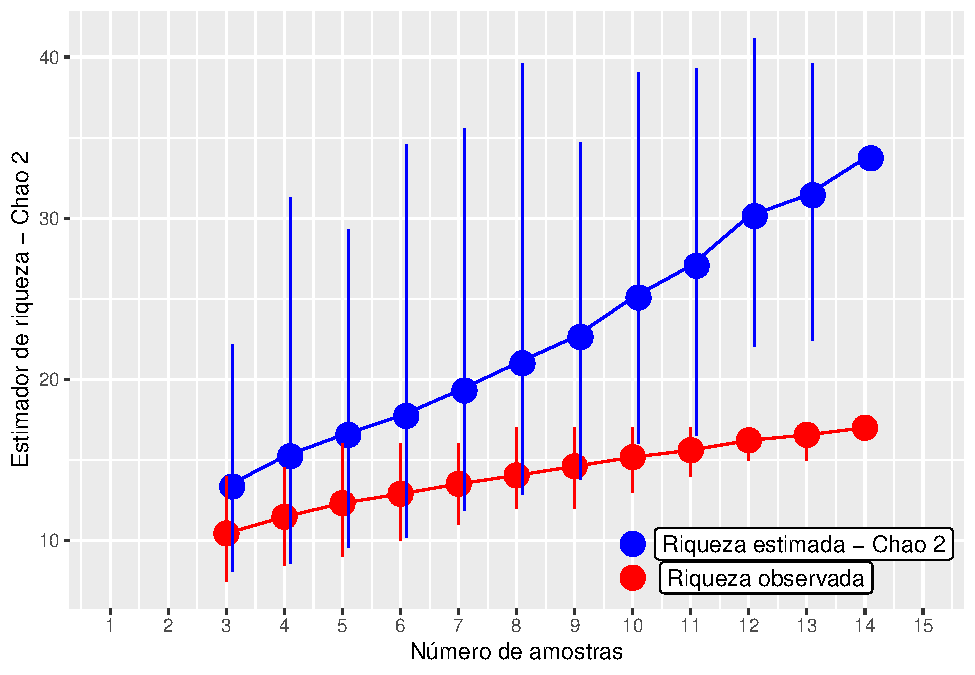
\includegraphics{livro_r_ecologia_files/figure-latex/unnamed-chunk-48-1.pdf}

\hypertarget{interpretauxe7uxe3o-dos-resultados-2}{%
\subsubsection{Interpretação dos resultados}\label{interpretauxe7uxe3o-dos-resultados-2}}

Com base no número de espécies raras (\emph{uniques} e \emph{duplicates}), Chao 2 estimou a possibilidade de encontrarmos mais dezesseis espécies caso o esforço amostral fosse maior e não mostrou tendência de estabilização da curva em uma assíntota.

\hypertarget{jackknife-1-burnham-overton-1978-1979}{%
\subsection{JACKKNIFE 1 (Burnham \& Overton 1978, 1979):}\label{jackknife-1-burnham-overton-1978-1979}}

Este estimador baseia-se no número de espécies que ocorrem em somente uma amostra (Q1).

\begin{quote}
\[S_{jack1} = S_{obs} + Q1\left(\frac{m - 1}{m}\right)\]
\end{quote}

onde:

\begin{itemize}
\item
  Sobs = o número de espécies na comunidade,
\item
  Q1 = número de espécies observadas em uma amostragem (espécies \emph{uniques}),
\item
  \emph{m} = número de amostragens.
\end{itemize}

Palmer (1990) verificou que Jackknife 1 foi o estimador mais preciso e menos enviesado comparado a outros métodos de extrapolação.

~

\hypertarget{exemplo-pruxe1tico---jackknife-1}{%
\subsubsection{Exemplo prático - Jackknife 1}\label{exemplo-pruxe1tico---jackknife-1}}

\hypertarget{explicauxe7uxe3o-dos-dados-3}{%
\paragraph{Explicação dos dados}\label{explicauxe7uxe3o-dos-dados-3}}

Usaremos os mesmos dados de 17 espécies de anuros amostradas em 14 dias de coletas de campo em um habitat reprodutivo localizado na região noroeste do estado de São Paulo, Brasil.

\textbf{Pergunta:}

\begin{quote}
Quantas espécies a mais poderiam ser amostradas caso aumentassemos o esforço amostral?
\end{quote}

\textbf{Predições}

\begin{quote}
\begin{itemize}
\tightlist
\item
  O número de espécies estimadas é similar ao número de espécies observada;
\item
  O número de espécies estimadas é maior do que o número de espécies observada.
\end{itemize}
\end{quote}

\textbf{Variáveis}

\begin{itemize}
\tightlist
\item
  Variáveis preditoras

  \begin{itemize}
  \tightlist
  \item
    matriz ou vetor com as abundâncias das espécies de anuros registradas em um habitat reprodutivo
  \end{itemize}
\end{itemize}

\textbf{Checklist}

\begin{itemize}
\tightlist
\item
  Verificar se a sua matriz está com as espécies nas colunas e as amostragens nas linhas
\end{itemize}

\hypertarget{anuxe1lise-3}{%
\subsection{Análise}\label{anuxe1lise-3}}

Calculo do estimador de riqueza - Jackknife 1

\begin{Shaded}
\begin{Highlighting}[]
\KeywordTok{library}\NormalTok{(vegan)}
\NormalTok{dados_coleta <-}\StringTok{ }\NormalTok{poca_anuros}
\NormalTok{est_jack1 <-}\StringTok{ }\KeywordTok{poolaccum}\NormalTok{(dados_coleta, }\DataTypeTok{permutations =} \DecValTok{100}\NormalTok{)}
\KeywordTok{summary}\NormalTok{(est_jack1, }\DataTypeTok{display =} \StringTok{"jack1"}\NormalTok{)}
\end{Highlighting}
\end{Shaded}

\begin{verbatim}
## $jack1
##        N Jackknife 1      2.5%    97.5%  Std.Dev
##  [1,]  3    13.82667  8.666667 18.84167 2.950957
##  [2,]  4    14.78500  8.712500 19.64375 2.957404
##  [3,]  5    15.56800 10.180000 21.02000 2.943470
##  [4,]  6    16.52833 11.229167 20.92083 2.645439
##  [5,]  7    17.06143 12.264286 22.00000 2.777628
##  [6,]  8    17.70375 13.225000 22.65000 2.613802
##  [7,]  9    18.79000 14.666667 24.11111 2.666101
##  [8,] 10    19.54500 14.747500 23.77250 2.577697
##  [9,] 11    20.38273 14.818182 23.36364 2.440931
## [10,] 12    21.30750 17.185417 23.41667 1.934850
## [11,] 13    21.86000 18.692308 23.46154 1.483815
## [12,] 14    22.57143 22.571429 22.57143 0.000000
## 
## attr(,"class")
## [1] "summary.poolaccum"
\end{verbatim}

Visualizar os resultados com 95\% intervalo de confiança

\begin{Shaded}
\begin{Highlighting}[]
\KeywordTok{library}\NormalTok{(ggplot2)}
\CommentTok{# preparando os dados para fazer o gráfico}
\NormalTok{resultados_jack1 <-}\StringTok{ }\KeywordTok{summary}\NormalTok{(est_jack1, }\DataTypeTok{display =} \KeywordTok{c}\NormalTok{(}\StringTok{"S"}\NormalTok{, }\StringTok{"jack1"}\NormalTok{))}
\NormalTok{res_jack1 <-}\StringTok{ }\KeywordTok{cbind}\NormalTok{(resultados_jack1}\OperatorTok{$}\NormalTok{jack1[,}\DecValTok{1}\OperatorTok{:}\DecValTok{4}\NormalTok{], resultados_jack1}\OperatorTok{$}\NormalTok{S[,}\DecValTok{2}\OperatorTok{:}\DecValTok{4}\NormalTok{])}
\NormalTok{res_jack1 <-}\StringTok{ }\KeywordTok{as.data.frame}\NormalTok{(res_jack1)}
\KeywordTok{colnames}\NormalTok{(res_jack1) <-}\StringTok{ }\KeywordTok{c}\NormalTok{(}\StringTok{"Amostras"}\NormalTok{, }\StringTok{"JACK1"}\NormalTok{, }\StringTok{"JACK1_inferior"}\NormalTok{, }\StringTok{"JACK1_superior"}\NormalTok{, }\StringTok{"Riqueza"}\NormalTok{,}
                        \StringTok{"R_inferior"}\NormalTok{, }\StringTok{"R_superior"}\NormalTok{)}

\CommentTok{# comando para o gráfico}
\KeywordTok{ggplot}\NormalTok{(res_jack1, }\KeywordTok{aes}\NormalTok{(}\DataTypeTok{y =}\NormalTok{ Riqueza, }\DataTypeTok{x =}\NormalTok{ Amostras)) }\OperatorTok{+}
\StringTok{  }\KeywordTok{geom_point}\NormalTok{(}\KeywordTok{aes}\NormalTok{(}\DataTypeTok{y =}\NormalTok{ JACK1, }\DataTypeTok{x =}\NormalTok{ Amostras }\OperatorTok{+}\StringTok{ }\FloatTok{0.1}\NormalTok{), }\DataTypeTok{size =} \DecValTok{5}\NormalTok{, }\DataTypeTok{color =} \StringTok{"blue"}\NormalTok{, }\DataTypeTok{alpha =} \DecValTok{1}\NormalTok{) }\OperatorTok{+}
\StringTok{  }\KeywordTok{geom_point}\NormalTok{(}\KeywordTok{aes}\NormalTok{(}\DataTypeTok{y =}\NormalTok{ Riqueza, }\DataTypeTok{x =}\NormalTok{ Amostras), }\DataTypeTok{size =} \DecValTok{5}\NormalTok{, }\DataTypeTok{color =} \StringTok{"red"}\NormalTok{, }\DataTypeTok{alpha =} \DecValTok{1}\NormalTok{) }\OperatorTok{+}
\StringTok{  }\KeywordTok{geom_line}\NormalTok{ (}\KeywordTok{aes}\NormalTok{(}\DataTypeTok{y =}\NormalTok{ JACK1, }\DataTypeTok{x =}\NormalTok{ Amostras), }\DataTypeTok{color =} \StringTok{"blue"}\NormalTok{) }\OperatorTok{+}
\StringTok{  }\KeywordTok{geom_line}\NormalTok{ (}\KeywordTok{aes}\NormalTok{(}\DataTypeTok{y =}\NormalTok{ Riqueza, }\DataTypeTok{x =}\NormalTok{ Amostras), }\DataTypeTok{color =} \StringTok{"red"}\NormalTok{) }\OperatorTok{+}
\StringTok{  }\KeywordTok{geom_linerange}\NormalTok{(}\KeywordTok{aes}\NormalTok{(}\DataTypeTok{ymin =}\NormalTok{ JACK1_inferior, }\DataTypeTok{ymax =}\NormalTok{ JACK1_superior, }\DataTypeTok{x =}\NormalTok{ Amostras }\OperatorTok{+}\StringTok{ }\FloatTok{0.1}\NormalTok{),}
 \DataTypeTok{color =} \StringTok{"blue"}\NormalTok{) }\OperatorTok{+}
\StringTok{  }\KeywordTok{geom_linerange}\NormalTok{(}\KeywordTok{aes}\NormalTok{(}\DataTypeTok{ymin =}\NormalTok{ R_inferior, }\DataTypeTok{ymax =}\NormalTok{ R_superior, }\DataTypeTok{x =}\NormalTok{ Amostras), }\DataTypeTok{color =} \StringTok{"red"}\NormalTok{) }\OperatorTok{+}
\StringTok{  }\KeywordTok{ylab}\NormalTok{ (}\StringTok{"Estimador de riqueza - Jackknife 1"}\NormalTok{) }\OperatorTok{+}
\StringTok{  }\KeywordTok{xlab}\NormalTok{ (}\StringTok{"Número de amostras"}\NormalTok{) }\OperatorTok{+}
\StringTok{  }\KeywordTok{scale_x_continuous}\NormalTok{(}\DataTypeTok{limits =} \KeywordTok{c}\NormalTok{(}\DecValTok{1}\NormalTok{,}\DecValTok{15}\NormalTok{), }\DataTypeTok{breaks=}\KeywordTok{seq}\NormalTok{(}\DecValTok{1}\NormalTok{,}\DecValTok{15}\NormalTok{,}\DecValTok{1}\NormalTok{)) }\OperatorTok{+}
\StringTok{  }\KeywordTok{geom_point}\NormalTok{(}\DataTypeTok{y=} \FloatTok{9.9}\NormalTok{, }\DataTypeTok{x =} \DecValTok{9}\NormalTok{, }\DataTypeTok{size =} \DecValTok{5}\NormalTok{, }\DataTypeTok{color =} \StringTok{"blue"}\NormalTok{, }\DataTypeTok{alpha =} \DecValTok{1}\NormalTok{) }\OperatorTok{+}\StringTok{ }
\StringTok{  }\KeywordTok{geom_point}\NormalTok{(}\DataTypeTok{y=} \FloatTok{8.6}\NormalTok{, }\DataTypeTok{x =} \DecValTok{9}\NormalTok{, }\DataTypeTok{size =} \DecValTok{5}\NormalTok{, }\DataTypeTok{color =} \StringTok{"red"}\NormalTok{, }\DataTypeTok{alpha =} \DecValTok{1}\NormalTok{) }\OperatorTok{+}\StringTok{ }
\StringTok{  }\KeywordTok{geom_label}\NormalTok{( }\DataTypeTok{y =} \FloatTok{9.9}\NormalTok{, }\DataTypeTok{x =} \FloatTok{12.5}\NormalTok{, }\DataTypeTok{label =} \StringTok{"Riqueza estimada - Jackknife 1"}\NormalTok{) }\OperatorTok{+}
\StringTok{  }\KeywordTok{geom_label}\NormalTok{( }\DataTypeTok{y =} \FloatTok{8.6}\NormalTok{, }\DataTypeTok{x =} \FloatTok{11.5}\NormalTok{, }\DataTypeTok{label =} \StringTok{"Riqueza observada"}\NormalTok{)}
\end{Highlighting}
\end{Shaded}

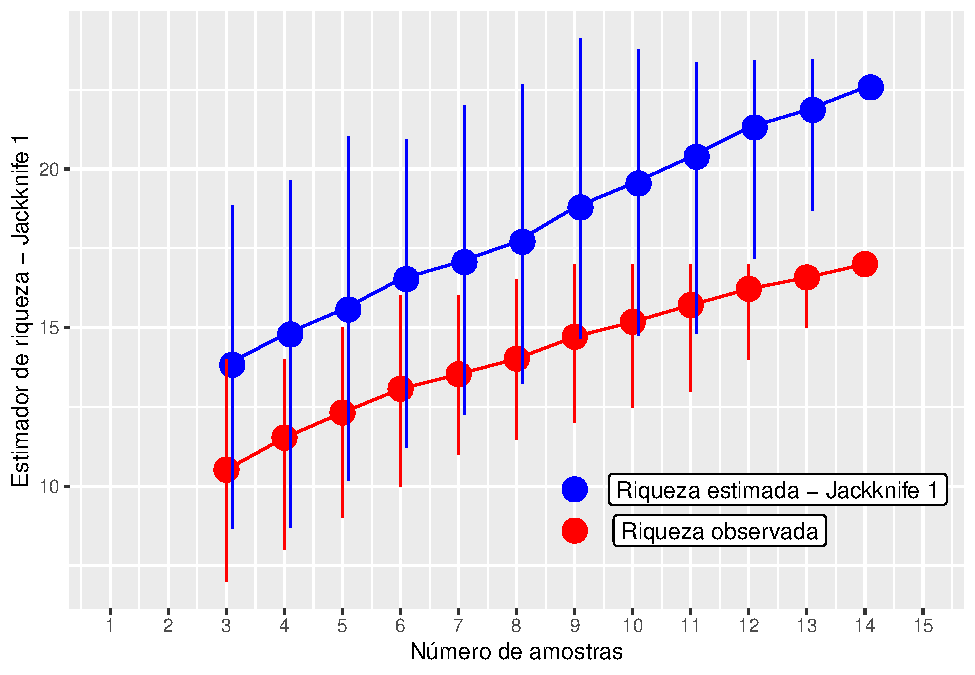
\includegraphics{livro_r_ecologia_files/figure-latex/unnamed-chunk-50-1.pdf}

\hypertarget{interpretauxe7uxe3o-dos-resultados-3}{%
\subsubsection{Interpretação dos resultados}\label{interpretauxe7uxe3o-dos-resultados-3}}

Com base no número de espécies raras, o estimador Jackknife 1 calculou a possibilidade de encontrarmos mais seis espécies caso o esforço amostral fosse maior e não mostrou tendência de estabilização da curva em uma assíntota.

\hypertarget{jackknife-2-burnham-overton-1978-1979-palmer-1991}{%
\subsection{JACKKNIFE 2 (Burnham \& Overton 1978, 1979, Palmer 1991):}\label{jackknife-2-burnham-overton-1978-1979-palmer-1991}}

Este método basea-se no número de espécies que ocorrem em apenas uma amostra e no número de espécies que ocorrem em exatamente duas amostras.

\begin{quote}
\[S_{jack2} = S_{obs} + \left[\frac{Q_1(2m - 3)}{m}-\frac{Q_2(m - 2)^2}{m(m-1)}\right]\]
\end{quote}

onde:

\begin{itemize}
\item
  Sobs = o número de espécies na comunidade,
\item
  \emph{m} = número de amostragens,
\item
  Q1 = número de espécies observadas em uma amostragem (espécies \emph{uniques}),
\item
  Q2 = número de espécies observadas em duas amostragens (espécies \emph{duplicates}).
\end{itemize}

~

\hypertarget{exemplo-pruxe1tico---jackknife-2}{%
\subsubsection{Exemplo prático - Jackknife 2}\label{exemplo-pruxe1tico---jackknife-2}}

\hypertarget{explicauxe7uxe3o-dos-dados-4}{%
\paragraph{Explicação dos dados}\label{explicauxe7uxe3o-dos-dados-4}}

Usaremos os mesmos dados de 17 espécies de anuros amostradas em 14 dias de coletas de campo em um habitat reprodutivo localizado na região noroeste do estado de São Paulo, Brasil.

\textbf{Pergunta:}

\begin{quote}
Quantas espécies a mais poderiam ser amostradas caso aumentassemos o esforço amostral?
\end{quote}

\textbf{Predições}

\begin{quote}
\begin{itemize}
\tightlist
\item
  O número de espécies estimadas é similar ao número de espécies observada;
\item
  O número de espécies estimadas é maior do que o número de espécies observada.
\end{itemize}
\end{quote}

\textbf{Variáveis}

\begin{itemize}
\tightlist
\item
  Variáveis preditoras

  \begin{itemize}
  \tightlist
  \item
    matriz ou vetor com as abundâncias das espécies de anuros registradas em um habitat reprodutivo
  \end{itemize}
\end{itemize}

\textbf{Checklist}

\begin{itemize}
\tightlist
\item
  Verificar se a sua matriz está com as espécies nas colunas e as amostragens nas linhas
\end{itemize}

\hypertarget{anuxe1lise-4}{%
\subsection{Análise}\label{anuxe1lise-4}}

Calculo do estimador de riqueza - Jackknife 2

\begin{Shaded}
\begin{Highlighting}[]
\KeywordTok{library}\NormalTok{(vegan)}
\NormalTok{dados_coleta <-}\StringTok{ }\NormalTok{poca_anuros}
\NormalTok{est_jack2 <-}\StringTok{ }\KeywordTok{poolaccum}\NormalTok{(dados_coleta, }\DataTypeTok{permutations =} \DecValTok{100}\NormalTok{)}
\KeywordTok{summary}\NormalTok{(est_jack2, }\DataTypeTok{display =} \StringTok{"jack2"}\NormalTok{)}
\end{Highlighting}
\end{Shaded}

\begin{verbatim}
## $jack2
##        N Jackknife 2      2.5%    97.5%  Std.Dev
##  [1,]  3    14.64500  8.158333 20.83333 3.202101
##  [2,]  4    15.60000  8.075000 22.08333 3.442163
##  [3,]  5    16.68050  9.477500 23.58625 4.091454
##  [4,]  6    17.69600  7.933333 25.93500 3.964985
##  [5,]  7    18.94429 12.952381 26.40476 3.669180
##  [6,]  8    20.07625 12.448661 27.56250 4.262035
##  [7,]  9    21.63444 12.739931 29.21840 4.206383
##  [8,] 10    22.62467 14.826111 30.60000 4.301085
##  [9,] 11    23.86518 15.331591 28.35455 3.696371
## [10,] 12    24.90167 18.492424 28.49242 2.930756
## [11,] 13    25.81147 21.301282 28.60897 2.112491
## [12,] 14    26.92308 26.923077 26.92308 0.000000
## 
## attr(,"class")
## [1] "summary.poolaccum"
\end{verbatim}

Visualizar os resultados com intervalo de confiança de 95\%

\begin{Shaded}
\begin{Highlighting}[]
\KeywordTok{library}\NormalTok{(ggplot2)}
\CommentTok{# preparando os dados para fazer o gráfico}
\NormalTok{resultados_jack2 <-}\StringTok{ }\KeywordTok{summary}\NormalTok{(est_jack2, }\DataTypeTok{display =} \KeywordTok{c}\NormalTok{(}\StringTok{"S"}\NormalTok{, }\StringTok{"jack2"}\NormalTok{))}
\NormalTok{res_jack2 <-}\StringTok{ }\KeywordTok{cbind}\NormalTok{(resultados_jack2}\OperatorTok{$}\NormalTok{jack2[,}\DecValTok{1}\OperatorTok{:}\DecValTok{4}\NormalTok{], resultados_jack2}\OperatorTok{$}\NormalTok{S[,}\DecValTok{2}\OperatorTok{:}\DecValTok{4}\NormalTok{])}
\NormalTok{res_jack2 <-}\StringTok{ }\KeywordTok{as.data.frame}\NormalTok{(res_jack2)}
\KeywordTok{colnames}\NormalTok{(res_jack2) <-}\StringTok{ }\KeywordTok{c}\NormalTok{(}\StringTok{"Amostras"}\NormalTok{, }\StringTok{"JACK2"}\NormalTok{, }\StringTok{"JACK2_inferior"}\NormalTok{, }\StringTok{"JACK2_superior"}\NormalTok{, }\StringTok{"Riqueza"}\NormalTok{,}
                        \StringTok{"R_inferior"}\NormalTok{, }\StringTok{"R_superior"}\NormalTok{)}

\CommentTok{# comando para o gráfico}
\KeywordTok{ggplot}\NormalTok{(res_jack2, }\KeywordTok{aes}\NormalTok{(}\DataTypeTok{y =}\NormalTok{ Riqueza, }\DataTypeTok{x =}\NormalTok{ Amostras)) }\OperatorTok{+}
\StringTok{  }\KeywordTok{geom_point}\NormalTok{(}\KeywordTok{aes}\NormalTok{(}\DataTypeTok{y =}\NormalTok{ JACK2, }\DataTypeTok{x =}\NormalTok{ Amostras }\OperatorTok{+}\StringTok{ }\FloatTok{0.1}\NormalTok{), }\DataTypeTok{size =} \DecValTok{5}\NormalTok{, }\DataTypeTok{color =} \StringTok{"blue"}\NormalTok{, }\DataTypeTok{alpha =} \DecValTok{1}\NormalTok{) }\OperatorTok{+}
\StringTok{  }\KeywordTok{geom_point}\NormalTok{(}\KeywordTok{aes}\NormalTok{(}\DataTypeTok{y =}\NormalTok{ Riqueza, }\DataTypeTok{x =}\NormalTok{ Amostras), }\DataTypeTok{size =} \DecValTok{5}\NormalTok{, }\DataTypeTok{color =} \StringTok{"red"}\NormalTok{, }\DataTypeTok{alpha =} \DecValTok{1}\NormalTok{) }\OperatorTok{+}
\StringTok{  }\KeywordTok{geom_line}\NormalTok{ (}\KeywordTok{aes}\NormalTok{(}\DataTypeTok{y =}\NormalTok{ JACK2, }\DataTypeTok{x =}\NormalTok{ Amostras), }\DataTypeTok{color =} \StringTok{"blue"}\NormalTok{) }\OperatorTok{+}
\StringTok{  }\KeywordTok{geom_line}\NormalTok{ (}\KeywordTok{aes}\NormalTok{(}\DataTypeTok{y =}\NormalTok{ Riqueza, }\DataTypeTok{x =}\NormalTok{ Amostras), }\DataTypeTok{color =} \StringTok{"red"}\NormalTok{) }\OperatorTok{+}
\StringTok{  }\KeywordTok{geom_linerange}\NormalTok{(}\KeywordTok{aes}\NormalTok{(}\DataTypeTok{ymin =}\NormalTok{ JACK2_inferior, }\DataTypeTok{ymax =}\NormalTok{ JACK2_superior, }\DataTypeTok{x =}\NormalTok{ Amostras }\OperatorTok{+}\StringTok{ }\FloatTok{0.1}\NormalTok{),}
 \DataTypeTok{color =} \StringTok{"blue"}\NormalTok{) }\OperatorTok{+}
\StringTok{  }\KeywordTok{geom_linerange}\NormalTok{(}\KeywordTok{aes}\NormalTok{(}\DataTypeTok{ymin =}\NormalTok{ R_inferior, }\DataTypeTok{ymax =}\NormalTok{ R_superior, }\DataTypeTok{x =}\NormalTok{ Amostras), }\DataTypeTok{color =} \StringTok{"red"}\NormalTok{) }\OperatorTok{+}
\StringTok{  }\KeywordTok{ylab}\NormalTok{ (}\StringTok{"Estimador de riqueza - Jackknife 2"}\NormalTok{) }\OperatorTok{+}
\StringTok{  }\KeywordTok{xlab}\NormalTok{ (}\StringTok{"Número de amostras"}\NormalTok{) }\OperatorTok{+}
\StringTok{  }\KeywordTok{scale_x_continuous}\NormalTok{(}\DataTypeTok{limits =} \KeywordTok{c}\NormalTok{(}\DecValTok{1}\NormalTok{,}\DecValTok{15}\NormalTok{), }\DataTypeTok{breaks=}\KeywordTok{seq}\NormalTok{(}\DecValTok{1}\NormalTok{,}\DecValTok{15}\NormalTok{,}\DecValTok{1}\NormalTok{)) }\OperatorTok{+}
\StringTok{  }\KeywordTok{geom_point}\NormalTok{(}\DataTypeTok{y=} \FloatTok{9.9}\NormalTok{, }\DataTypeTok{x =} \DecValTok{9}\NormalTok{, }\DataTypeTok{size =} \DecValTok{5}\NormalTok{, }\DataTypeTok{color =} \StringTok{"blue"}\NormalTok{, }\DataTypeTok{alpha =} \DecValTok{1}\NormalTok{) }\OperatorTok{+}\StringTok{ }
\StringTok{  }\KeywordTok{geom_point}\NormalTok{(}\DataTypeTok{y=} \FloatTok{8.2}\NormalTok{, }\DataTypeTok{x =} \DecValTok{9}\NormalTok{, }\DataTypeTok{size =} \DecValTok{5}\NormalTok{, }\DataTypeTok{color =} \StringTok{"red"}\NormalTok{, }\DataTypeTok{alpha =} \DecValTok{1}\NormalTok{) }\OperatorTok{+}\StringTok{ }
\StringTok{  }\KeywordTok{geom_label}\NormalTok{( }\DataTypeTok{y =} \FloatTok{9.9}\NormalTok{, }\DataTypeTok{x =} \FloatTok{12.5}\NormalTok{, }\DataTypeTok{label =} \StringTok{"Riqueza estimada - Jackknife 2"}\NormalTok{) }\OperatorTok{+}
\StringTok{  }\KeywordTok{geom_label}\NormalTok{( }\DataTypeTok{y =} \FloatTok{8.2}\NormalTok{, }\DataTypeTok{x =} \FloatTok{11.5}\NormalTok{, }\DataTypeTok{label =} \StringTok{"Riqueza observada"}\NormalTok{)}
\end{Highlighting}
\end{Shaded}

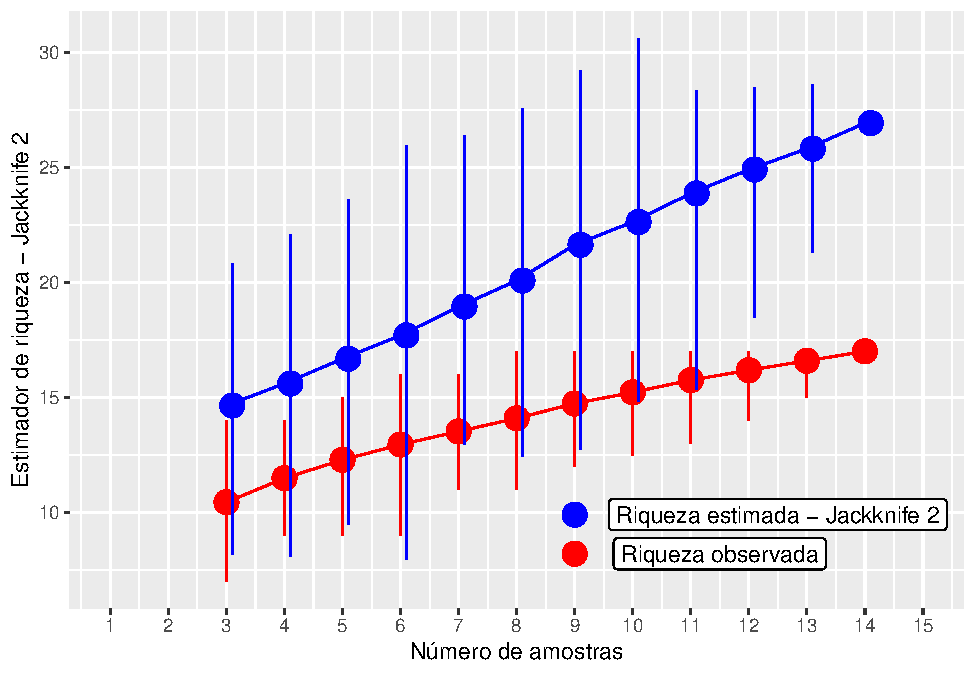
\includegraphics{livro_r_ecologia_files/figure-latex/unnamed-chunk-52-1.pdf}

\hypertarget{interpretauxe7uxe3o-dos-resultados-4}{%
\subsubsection{Interpretação dos resultados}\label{interpretauxe7uxe3o-dos-resultados-4}}

Com base no número de espécies raras, o estimador Jackknife 2 calculou a possibilidade de encontrarmos mais dez espécies caso o esforço amostral fosse maior e não mostrou tendência estabilização da curva em uma assíntota.

\hypertarget{bootstrap-smith-van-belle-1984}{%
\subsection{BOOTSTRAP (Smith \& van Belle 1984):}\label{bootstrap-smith-van-belle-1984}}

Este método difere dos demais por utilizar dados de todas as espécies coletadas para estimar a riqueza total, não se restringindo às espécies raras. Ele requer somente dados de incidência. A estimativa pelo bootstrap é calculada somando-se a riqueza observada à soma do inverso da proporção de amostras em que cada espécie ocorre.

\begin{quote}
\[S_{boot} = S_{obs} + \sum_{k=1}^{S_{obs}}(1-P_k)^m\]
\end{quote}

onde:

\begin{itemize}
\item
  Sobs = o número de espécies na comunidade,
\item
  \emph{m} = número de amostragens,
\item
  Pk = proporção do número de amostras em que cada espécie foi registrada.
\end{itemize}

~

\hypertarget{exemplo-pruxe1tico---bootstrap}{%
\subsubsection{Exemplo prático - Bootstrap}\label{exemplo-pruxe1tico---bootstrap}}

\hypertarget{explicauxe7uxe3o-dos-dados-5}{%
\paragraph{Explicação dos dados}\label{explicauxe7uxe3o-dos-dados-5}}

Usaremos os mesmos dados de 17 espécies de anuros amostradas em 14 dias de coletas de campo em um habitat reprodutivo localizado na região noroeste do estado de São Paulo, Brasil.

\textbf{Pergunta:}

\begin{quote}
Quantas espécies a mais poderiam ser amostradas caso aumentassemos o esforço amostral?
\end{quote}

\textbf{Predições}

\begin{quote}
\begin{itemize}
\tightlist
\item
  O número de espécies estimadas é similar ao número de espécies observada;
\item
  O número de espécies estimadas é maior do que o número de espécies observada.
\end{itemize}
\end{quote}

\textbf{Variáveis}

\begin{itemize}
\tightlist
\item
  Variáveis preditoras

  \begin{itemize}
  \tightlist
  \item
    matriz ou vetor com as abundâncias das espécies de anuros registradas em um habitat reprodutivo
  \end{itemize}
\end{itemize}

\textbf{Checklist}

\begin{itemize}
\tightlist
\item
  Verificar se a sua matriz está com as espécies nas colunas e as amostragens nas linhas
\end{itemize}

\hypertarget{anuxe1lise-5}{%
\subsection{Análise}\label{anuxe1lise-5}}

Calculo do estimador de riqueza - Bootstrap

\begin{Shaded}
\begin{Highlighting}[]
\KeywordTok{library}\NormalTok{(vegan)}
\NormalTok{dados_coleta <-}\StringTok{ }\NormalTok{poca_anuros}
\NormalTok{est_boot <-}\StringTok{ }\KeywordTok{poolaccum}\NormalTok{(dados_coleta, }\DataTypeTok{permutations =} \DecValTok{100}\NormalTok{)}
\KeywordTok{summary}\NormalTok{(est_boot, }\DataTypeTok{display =} \StringTok{"boot"}\NormalTok{)}
\end{Highlighting}
\end{Shaded}

\begin{verbatim}
## $boot
##        N Bootstrap      2.5%    97.5%   Std.Dev
##  [1,]  3  12.40852  7.176852 16.51852 2.4176418
##  [2,]  4  13.43441  9.704590 17.63779 2.2302298
##  [3,]  5  14.10795 10.028328 18.45547 2.1122632
##  [4,]  6  14.77651 10.792903 18.54641 1.9508799
##  [5,]  7  15.41704 12.327781 19.70504 1.8976136
##  [6,]  8  15.97237 12.672585 19.72559 1.8638363
##  [7,]  9  16.57902 13.451358 19.80904 1.8312781
##  [8,] 10  17.25744 14.061712 19.82072 1.7632069
##  [9,] 11  18.01725 15.229070 19.81428 1.4752163
## [10,] 12  18.41744 16.561405 19.58719 1.2210355
## [11,] 13  18.86269 16.570376 19.35010 0.8976061
## [12,] 14  19.27832 19.278321 19.27832 0.0000000
## 
## attr(,"class")
## [1] "summary.poolaccum"
\end{verbatim}

Visualizar os resultados com intervalo de confiança de 95\%

\begin{Shaded}
\begin{Highlighting}[]
\KeywordTok{library}\NormalTok{(ggplot2)}
\CommentTok{# preparando os dados para fazer o gráfico}
\NormalTok{resultados_boot <-}\StringTok{ }\KeywordTok{summary}\NormalTok{(est_boot, }\DataTypeTok{display =} \KeywordTok{c}\NormalTok{(}\StringTok{"S"}\NormalTok{, }\StringTok{"boot"}\NormalTok{))}
\NormalTok{res_boot <-}\StringTok{ }\KeywordTok{cbind}\NormalTok{(resultados_boot}\OperatorTok{$}\NormalTok{boot[,}\DecValTok{1}\OperatorTok{:}\DecValTok{4}\NormalTok{], resultados_boot}\OperatorTok{$}\NormalTok{S[,}\DecValTok{2}\OperatorTok{:}\DecValTok{4}\NormalTok{])}
\NormalTok{res_boot <-}\StringTok{ }\KeywordTok{as.data.frame}\NormalTok{(res_boot)}
\KeywordTok{colnames}\NormalTok{(res_boot) <-}\StringTok{ }\KeywordTok{c}\NormalTok{(}\StringTok{"Amostras"}\NormalTok{, }\StringTok{"BOOT"}\NormalTok{, }\StringTok{"BOOT_inferior"}\NormalTok{, }\StringTok{"BOOT_superior"}\NormalTok{, }\StringTok{"Riqueza"}\NormalTok{,}
                        \StringTok{"R_inferior"}\NormalTok{, }\StringTok{"R_superior"}\NormalTok{)}

\CommentTok{# comando para o gráfico}
\KeywordTok{ggplot}\NormalTok{(res_boot, }\KeywordTok{aes}\NormalTok{(}\DataTypeTok{y =}\NormalTok{ Riqueza, }\DataTypeTok{x =}\NormalTok{ Amostras)) }\OperatorTok{+}
\StringTok{  }\KeywordTok{geom_point}\NormalTok{(}\KeywordTok{aes}\NormalTok{(}\DataTypeTok{y =}\NormalTok{ BOOT, }\DataTypeTok{x =}\NormalTok{ Amostras }\OperatorTok{+}\StringTok{ }\FloatTok{0.1}\NormalTok{), }\DataTypeTok{size =} \DecValTok{5}\NormalTok{, }\DataTypeTok{color =} \StringTok{"blue"}\NormalTok{, }\DataTypeTok{alpha =} \DecValTok{1}\NormalTok{) }\OperatorTok{+}
\StringTok{  }\KeywordTok{geom_point}\NormalTok{(}\KeywordTok{aes}\NormalTok{(}\DataTypeTok{y =}\NormalTok{ Riqueza, }\DataTypeTok{x =}\NormalTok{ Amostras), }\DataTypeTok{size =} \DecValTok{5}\NormalTok{, }\DataTypeTok{color =} \StringTok{"red"}\NormalTok{, }\DataTypeTok{alpha =} \DecValTok{1}\NormalTok{) }\OperatorTok{+}
\StringTok{  }\KeywordTok{geom_line}\NormalTok{ (}\KeywordTok{aes}\NormalTok{(}\DataTypeTok{y =}\NormalTok{ BOOT, }\DataTypeTok{x =}\NormalTok{ Amostras), }\DataTypeTok{color =} \StringTok{"blue"}\NormalTok{) }\OperatorTok{+}
\StringTok{  }\KeywordTok{geom_line}\NormalTok{ (}\KeywordTok{aes}\NormalTok{(}\DataTypeTok{y =}\NormalTok{ Riqueza, }\DataTypeTok{x =}\NormalTok{ Amostras), }\DataTypeTok{color =} \StringTok{"red"}\NormalTok{) }\OperatorTok{+}
\StringTok{  }\KeywordTok{geom_linerange}\NormalTok{(}\KeywordTok{aes}\NormalTok{(}\DataTypeTok{ymin =}\NormalTok{ BOOT_inferior, }\DataTypeTok{ymax =}\NormalTok{ BOOT_superior, }\DataTypeTok{x =}\NormalTok{ Amostras }\OperatorTok{+}\StringTok{ }\FloatTok{0.1}\NormalTok{),}
 \DataTypeTok{color =} \StringTok{"blue"}\NormalTok{) }\OperatorTok{+}
\StringTok{  }\KeywordTok{geom_linerange}\NormalTok{(}\KeywordTok{aes}\NormalTok{(}\DataTypeTok{ymin =}\NormalTok{ R_inferior, }\DataTypeTok{ymax =}\NormalTok{ R_superior, }\DataTypeTok{x =}\NormalTok{ Amostras), }\DataTypeTok{color =} \StringTok{"red"}\NormalTok{) }\OperatorTok{+}
\StringTok{  }\KeywordTok{ylab}\NormalTok{ (}\StringTok{"Estimador de riqueza - Bootstrap"}\NormalTok{) }\OperatorTok{+}
\StringTok{  }\KeywordTok{xlab}\NormalTok{ (}\StringTok{"Número de amostras"}\NormalTok{) }\OperatorTok{+}
\StringTok{  }\KeywordTok{scale_x_continuous}\NormalTok{(}\DataTypeTok{limits =} \KeywordTok{c}\NormalTok{(}\DecValTok{1}\NormalTok{,}\DecValTok{15}\NormalTok{), }\DataTypeTok{breaks=}\KeywordTok{seq}\NormalTok{(}\DecValTok{1}\NormalTok{,}\DecValTok{15}\NormalTok{,}\DecValTok{1}\NormalTok{)) }\OperatorTok{+}
\StringTok{  }\KeywordTok{geom_point}\NormalTok{(}\DataTypeTok{y=} \FloatTok{10.4}\NormalTok{, }\DataTypeTok{x =} \FloatTok{9.5}\NormalTok{, }\DataTypeTok{size =} \DecValTok{5}\NormalTok{, }\DataTypeTok{color =} \StringTok{"blue"}\NormalTok{, }\DataTypeTok{alpha =} \DecValTok{1}\NormalTok{) }\OperatorTok{+}\StringTok{ }
\StringTok{  }\KeywordTok{geom_point}\NormalTok{(}\DataTypeTok{y=} \FloatTok{9.3}\NormalTok{, }\DataTypeTok{x =} \FloatTok{9.5}\NormalTok{, }\DataTypeTok{size =} \DecValTok{5}\NormalTok{, }\DataTypeTok{color =} \StringTok{"red"}\NormalTok{, }\DataTypeTok{alpha =} \DecValTok{1}\NormalTok{) }\OperatorTok{+}\StringTok{ }
\StringTok{  }\KeywordTok{geom_label}\NormalTok{( }\DataTypeTok{y =} \FloatTok{10.4}\NormalTok{, }\DataTypeTok{x =} \FloatTok{12.3}\NormalTok{, }\DataTypeTok{label =} \StringTok{"Riqueza estimada - Bootstrap"}\NormalTok{) }\OperatorTok{+}
\StringTok{  }\KeywordTok{geom_label}\NormalTok{( }\DataTypeTok{y =} \FloatTok{9.3}\NormalTok{, }\DataTypeTok{x =} \FloatTok{11.5}\NormalTok{, }\DataTypeTok{label =} \StringTok{"Riqueza observada"}\NormalTok{)}
\end{Highlighting}
\end{Shaded}

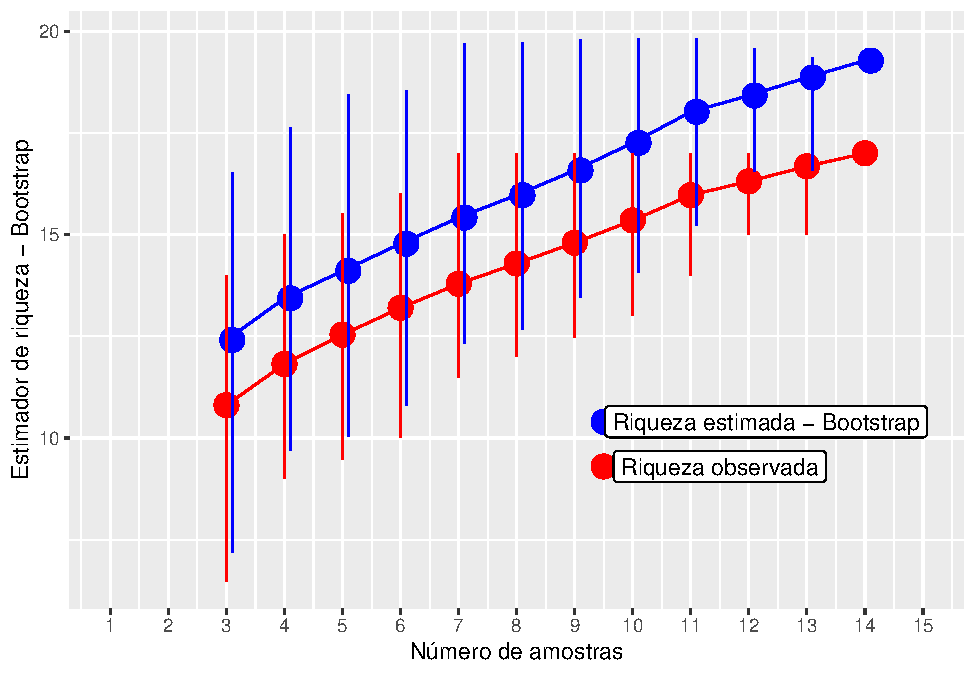
\includegraphics{livro_r_ecologia_files/figure-latex/unnamed-chunk-54-1.pdf}

\hypertarget{interpretauxe7uxe3o-dos-resultados-5}{%
\subsubsection{Interpretação dos resultados}\label{interpretauxe7uxe3o-dos-resultados-5}}

Com base na frequencia de ocorrência das espécies, o estimador bootstrap calculou a possibilidade de encontrarmos mais duas espécies caso o esforço amostral fosse maior e não mostrou tendência de estabilização da curva em uma assíntota.

\hypertarget{interpolauxe7uxe3o-e-extrapolauxe7uxe3o-baseadas-em-rarefauxe7uxe3o-usando-amostragens-de-inciduxeancia-ou-abunduxe2ncia-chao-jost-2012-colwell-et-al.-2012}{%
\subsection{Interpolação e Extrapolação baseadas em rarefação usando amostragens de incidência ou abundância (Chao \& Jost 2012, Colwell et al.~2012):}\label{interpolauxe7uxe3o-e-extrapolauxe7uxe3o-baseadas-em-rarefauxe7uxe3o-usando-amostragens-de-inciduxeancia-ou-abunduxe2ncia-chao-jost-2012-colwell-et-al.-2012}}

Este método utiliza teoria de amostragem (e.g.~modelos multinomial, Poisson e Bernoulli) para conectar rarefação (interpolação) e predição (extrapolação) com base no tamanho da amostra. Contudo, é importante enfatizar que a extrapolação torna-se altamente incerta quando extendida para o dobro do tamanho da amostragem. Este método utiliza uma abordagem com bootstrap para calcular o intervalo de confiança de 95\%. Uma das vantagens desta abordagem é que ela permite além da riqueza de espécies, interpolar e extrapolar os índices de diversidade de Shannon entropy (i.e.~quantifica a incerteza da identidade da espécie baseado na amostragem aleatória de um indivíduo da comunidade) e Gini-Simpson (i.e.~quantifica a probabilidade que dois indivíduos escolhidos aleatoriamente sejam de diferentes espécies). Contudo, estes índices de diversidades são transformados e apresentados em unidades de riqueza de espécies (\emph{Números de Hill}, Hill 1973). Hill percebeu que poderíamos calcular a riqueza de espécies máxima usando os índices de Shannon entropy e Gini-Simpson quando consideramos que todas as espécies na comunidade possuem abundâncias idênticas (máxima equitabilidade). Então, eles propos a transformação dos indíces de diversidade determinando qual seria o número de espécies equivalente da nossa comunidade (observado) se todas as espécies fossem igualmente abundantes (teórico). Desta maneira, os indíces podem ser comparavéis pois estão representados pela mesma unidade - riqueza de espécies. Os números de Hill são representados pelo parâmetro \emph{q} que controla a sensibilidide do índice em relação a abudância relativa das espécies (Gotelli \& Chao 2013). Quando q = 0 ele não considera a abundância das espécies e é igual a riqueza de espécies. Quando q = 1 ele é o exponencial da diversidade de Shannon, que dá uma peso maior para as espécies raras. Quando q = 2 ele é a diversidade de Simpson, que dá um peso maior para as espécies mais comuns na comunidade.

\hypertarget{exemplo-pruxe1tico}{%
\subsubsection{Exemplo prático}\label{exemplo-pruxe1tico}}

\hypertarget{explicauxe7uxe3o-dos-dados-6}{%
\paragraph{Explicação dos dados}\label{explicauxe7uxe3o-dos-dados-6}}

Usaremos os mesmos dados de 17 espécies de anuros amostradas em 14 dias de coletas de campo em um habitat reprodutivo localizado na região noroeste do estado de São Paulo, Brasil.

\textbf{Pergunta:}

\begin{quote}
Quantas espécies a mais poderiam ser amostradas caso aumentassemos o esforço amostral?
\end{quote}

\textbf{Predições}

\begin{quote}
\begin{itemize}
\tightlist
\item
  O número de espécies estimadas é similar ao número de espécies observada;
\item
  O número de espécies estimadas é maior do que o número de espécies observada.
\end{itemize}
\end{quote}

\textbf{Variáveis}

\begin{itemize}
\tightlist
\item
  Variáveis preditoras

  \begin{itemize}
  \tightlist
  \item
    matriz ou vetor com as abundâncias das espécies de anuros registradas em um habitat reprodutivo
  \end{itemize}
\end{itemize}

\textbf{Checklist}

\begin{itemize}
\tightlist
\item
  Verificar se a sua matriz está com as espécies nas colunas e as amostragens nas linhas.
\end{itemize}

\hypertarget{anuxe1lise-6}{%
\subsection{Análise}\label{anuxe1lise-6}}

Calculo da extrapolação da riqueza com base no número de indivíduos

\begin{Shaded}
\begin{Highlighting}[]
\KeywordTok{library}\NormalTok{(iNEXT)}
\NormalTok{dados_coleta <-}\StringTok{ }\NormalTok{poca_anuros}

\CommentTok{# preparando os dados para análises considerando a abundância}
\NormalTok{dados_inext_abu <-}\StringTok{ }\KeywordTok{colSums}\NormalTok{(dados_coleta) }

\NormalTok{resultados_abundancia <-}\StringTok{ }\KeywordTok{iNEXT}\NormalTok{(dados_inext_abu, }\DataTypeTok{q =} \DecValTok{0}\NormalTok{, }\DataTypeTok{datatype =} \StringTok{"abundance"}\NormalTok{, }
			\DataTypeTok{endpoint =} \DecValTok{600}\NormalTok{)}

\CommentTok{# Visualizar os dados no gráfico}
\KeywordTok{ggiNEXT}\NormalTok{(resultados_abundancia, }\DataTypeTok{type =} \DecValTok{1}\NormalTok{)}
\end{Highlighting}
\end{Shaded}

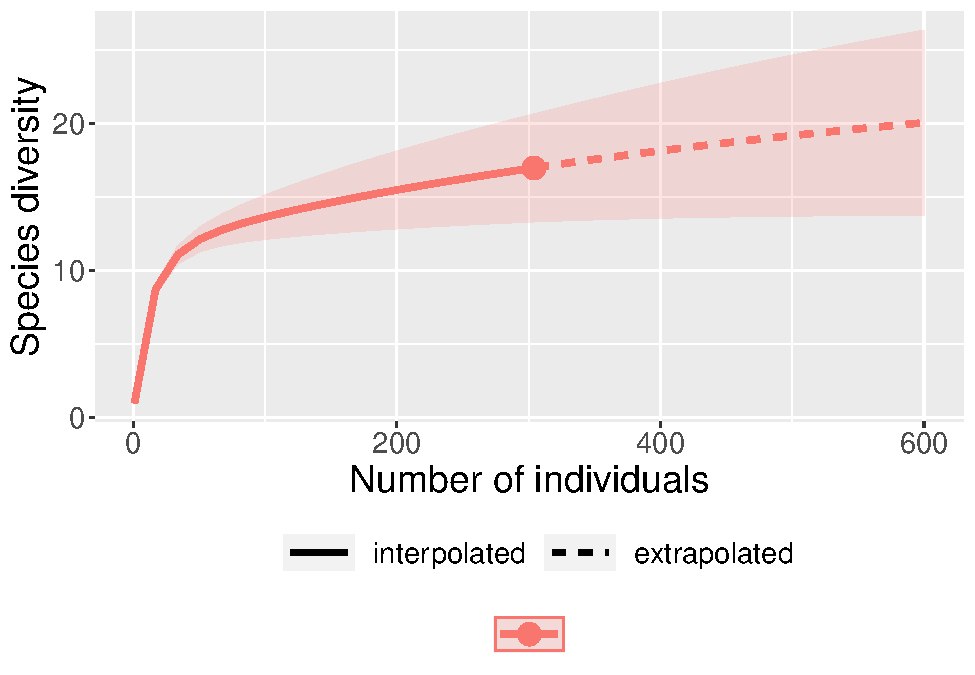
\includegraphics{livro_r_ecologia_files/figure-latex/unnamed-chunk-55-1.pdf}

\hypertarget{interpretauxe7uxe3o-dos-resultados-6}{%
\subsubsection{Interpretação dos resultados}\label{interpretauxe7uxe3o-dos-resultados-6}}

Veja que o ponto no final da linha contínua representa as 17 espécies de anuros (eixo Y) observadas entre os 304 individuos (eixo X). A extrapolação máxima (600 indivíduos no nosso exemplo), estima um aumento de até oito espécies (intervalo de confiança) caso amostrássemos mais 300 indivíduos.

Calculo da extrapolação da riqueza com base no número de amostras

\begin{Shaded}
\begin{Highlighting}[]
\KeywordTok{library}\NormalTok{(iNEXT)}
\NormalTok{dados_coleta <-}\StringTok{ }\NormalTok{poca_anuros}

\CommentTok{# preparando os dados para análises considerando a incidência}
\NormalTok{dados_inext <-}\StringTok{ }\KeywordTok{as.incfreq}\NormalTok{(}\KeywordTok{t}\NormalTok{(dados_coleta)) }\CommentTok{# preciso transpor o dataframe}

\NormalTok{resultados_incidencia <-}\StringTok{ }\KeywordTok{iNEXT}\NormalTok{(dados_inext, }\DataTypeTok{q =} \DecValTok{0}\NormalTok{, }\DataTypeTok{datatype =} \StringTok{"incidence_freq"}\NormalTok{, }
			\DataTypeTok{endpoint =} \DecValTok{30}\NormalTok{)}

\CommentTok{# Visualizar os dados no gráfico}
\KeywordTok{ggiNEXT}\NormalTok{(resultados_incidencia, }\DataTypeTok{type =} \DecValTok{1}\NormalTok{)}
\end{Highlighting}
\end{Shaded}

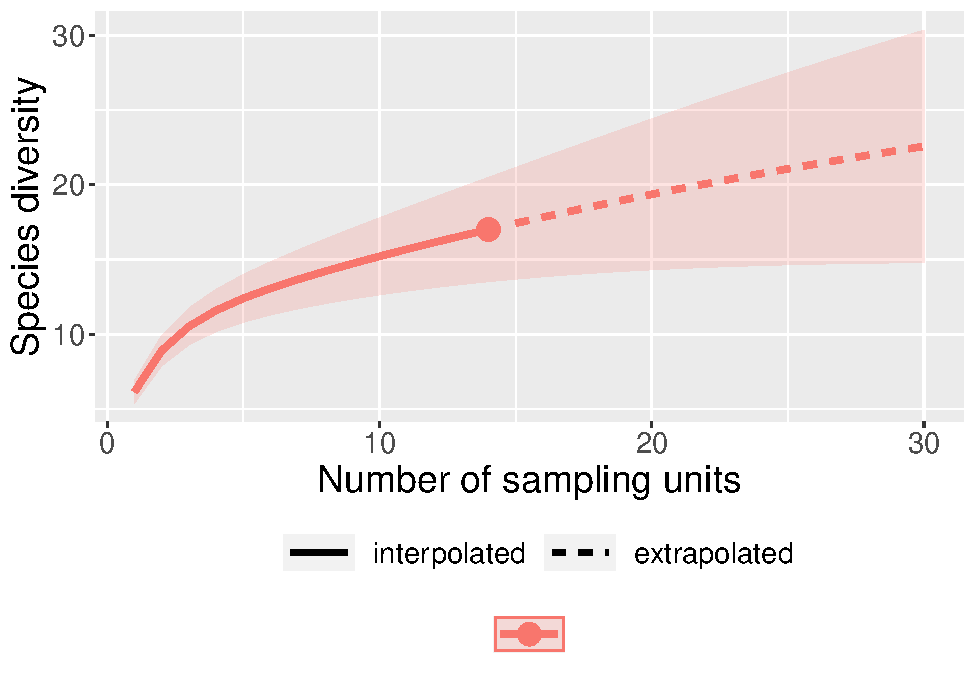
\includegraphics{livro_r_ecologia_files/figure-latex/unnamed-chunk-56-1.pdf}

\hypertarget{interpretauxe7uxe3o-dos-resultados-7}{%
\subsubsection{Interpretação dos resultados}\label{interpretauxe7uxe3o-dos-resultados-7}}

Veja que o ponto no final da linha contínua representa as 17 espécies de anuros (eixo Y) observadas nos 14 dias de coleta (eixo X - amostras). A extrapolação máxima (30 dias de coleta no nosso exemplo), estima um aumento de até 13 espécies (intervalo de confiança) caso amostrássemos mais 16 dias.

~

\hypertarget{para-se-aprofundar}{%
\subsection{Para se aprofundar}\label{para-se-aprofundar}}

\begin{itemize}
\item
  Recomendamos aos interessados que olhem a página do \href{http://viceroy.eeb.uconn.edu/estimates}{EstimateS software} e baixem o manual do usuário que contém informações detalhadas sobre os índices de rarefação e estimadores de riqueza.Este site foi criado e é mantido pelo Dr.~Robert K. Colwell, um dos maiores especialistas do mundo em estimativas da biodiversidade
\item
  Recomendamos também o livro Magurran \& McGill (2010) - Biological Diversity Frontiers in Measurement and Assessment.
\end{itemize}

  \bibliography{book.bib,packages.bib}

\end{document}
